\documentclass[11pt]{article}
\usepackage[table,xcdraw,dvipsnames]{xcolor}
\usepackage{multirow}
\usepackage{blindtext}
\usepackage[utf8]{inputenc}
\usepackage{listings}
\usepackage{mathtools}
\usepackage{graphicx}
\usepackage{matlab-prettifier}
\usepackage{subcaption}
\usepackage[margin=1.3in]{geometry}
\addtolength{\topmargin}{-.5in}
\linespread{1}
\usepackage{setspace}
\usepackage{fancybox}
\usepackage{amsmath}% http://ctan.org/pkg/amsmath
\usepackage{array}
\usepackage{tabu}
\usepackage{bm}
\usepackage{float}
\usepackage[export]{adjustbox}
\usepackage{wrapfig}
\usepackage[titletoc]{appendix}
\usepackage{listings}             % Include the listings-package
\setlength{\parindent}{0pt}
\bibliographystyle{IEEEtran}
\captionsetup{justification=centering}

\lstset{language=Java,
basicstyle=\ttfamily\scriptsize,
keywordstyle=\color{javapurple}\bfseries,
stringstyle=\color{javared},
commentstyle=\color{javagreen},
morecomment=[s][\color{javadocblue}]{/**}{*/},
numbers=left,
numberstyle=\tiny\color{black},
stepnumber=2,
numbersep=10pt,
tabsize=4,
showspaces=false,
showstringspaces=false,
breaklines=true,
frame=single}

\definecolor{grey}{rgb}{0.9,0.9,0.9} % Color of the box surrounding the title - these values can be changed to give the box a different color

\definecolor{javared}{rgb}{0.6,0,0} % for strings
\definecolor{javagreen}{rgb}{0.25,0.5,0.35} % comments
\definecolor{javapurple}{rgb}{0.5,0,0.35} % keywords
\definecolor{javadocblue}{rgb}{0.25,0.35,0.75} % javadoc

\makeatletter
\newcommand*{\rom}[1]{\expandafter\@slowromancap\romannumeral #1@}
\makeatother

\thispagestyle{empty}

\date{16 March 2017}

\begin{document}
\vspace*{6cm}
\colorbox{white}{
	\parbox[t]{1.0\linewidth}{
		\centering \fontsize{50pt}{80pt}\selectfont % The first argument for fontsize is the font size of the text and the second is the line spacing - you may need to play with these for your particular title
		\vspace*{0.7cm} % Space between the start of the title and the top of the grey box

		{401I - Final Year Project} \break
		\vspace*{0.7cm}
		Final Report
		\break
		Voice Recognition RPG
		\break
		Baron Khan (bak14)
		\vspace*{0.7cm} % Space between the end of the title and the bottom of the grey box
	}
}
\vfill % Space between the title box and author information




\newpage
\thispagestyle{empty}
\tableofcontents
\newpage
\setcounter{page}{1}
\section{Abstract}

\textbf{When adding voice commands to a video game, a developer may find themselves hard-coding text strings for phrases that a player can say, and mapping them to intents within the game. It becomes more work to include varying phrases of the same intent as the developer would have to include every permutation of the phrase (for which there could be infinitely many).
\\
\\
This project presents a text-based role-playing game (RPG) on Android which allows the player to issue actions within the game using their voice. The game uses a new voice recognition system that aims to make it easier for the developer to add voice commands without hard-coding the phrases, and with no cloud processing required. The system uses the WordNet database created by Princeton University to process voice commands.
\\
\\
Various techniques for improving the voice recognition system are explored and evaluated, with the aim of decreasing the developer workload. These include using semantic similarity methods, learning mechanisms, and more. The voice recognition system is also applied to other domains such as video conferencing solutions, and cooking applications.
\\
\\
This project also explores other areas for easing the development of the RPG, such as automatically assigning properties to objects, and room generation from text descriptions.}

\newpage

\section{Acknowledgements}

With thanks to Dr. Mark J. Wheelhouse of the Department of Computing at Imperial College London, for his guidance and supervision over this project.
\\
\\
Also many thanks to my family and friends for all their support.

\newpage

\section{Introduction}
In recent years, video games have explored various forms of input that diverge from the traditional control schemes of a keyboard and mouse, or an analogue stick and buttons on a controller. Touch-screen controls and motion controls have had varying degrees of success over the years, and provide new forms of interactions with games. A recent form of input used in video games has been voice controls; a user utters a sentence or phrase and this would execute an action or intent within the game.
\\
\\
Voice recognition and control schemes have been used in various ways in the medium, whether in tandem with traditional control schemes, or as the only form of input. Most games which feature a voice control scheme are typically programmed to work with a specific set of keywords or phrases, hard-coded by the developer. This is usually the case with games where the voice control interface is entirely optional to the user, as it requires little to no input from the programmer; if the speech processing is handled by a separate library, the developer just has to map a text string (e.g. ``open the door'') to the function that executes the intent (e.g. the function that opens a nearby door in the game).

\subsection{Role-Playing Games}

Role-playing games (RPG) are a genre of video games that involve the player controlling a character in a world featuring exploration and/or battle mechanics, along with a progression system, where the character gains new abilities or items as the game progresses. These include turn-based games such as Pok\'emon and Final Fantasy, or more action-based games such as Dark Souls and The Elder Scrolls.
\\
\\
In RPGs, the player usually possesses several items that they acquire during the game, and accesses them by navigating menus. If the player has many different items, they may need to spend a lot of time searching the menus for a specific item, which can be quite tedious. It can also become quite repetitive if the user is constantly only pushing the ``attack'' button over and over again with no variation in the attack used. Using voice commands, a player could just simply say a phrase such as, ``use a potion'' or, ``attack with an axe'', and the item will be used without having the player navigate several menu screens.

\subsection{Problem Statement}

It becomes increasingly difficult for a developer to add more phrases that can be accepted in the game and map to the same intent (e.g. when the user says, ``push the door open'' instead of, "open the door") as they would have to hard-code each possible input that the user could possibly say: having too few phrases would mean that the user could become frustrated when their preferred way of stating an intent is not accepted by the game, while adding too many acceptable phrases would increase development time.
\\
\\
Natural Language Processing (NLP) has been used to attempt to understand what users have said, and to extract meaning from the user's phrases and sentences. For instance, if the user says, ``push the door open'', NLP can be used to infer that the user's intent is to open a door. Using NLP, several user phrases can be mapped to the same intent without having to hard-code each possible phrase.
\\
\\
This project will apply NLP to a voice control scheme used within a role-playing game, in order to reduce the amount of work required by a developer to add a flexible voice control interface, and to give more freedom of expression to the player while they play the game.

\subsection{Motivation}

NLP is already used to improve voice recognition in popular personal assistants such as Siri or Alexa, but these systems offload the NLP workload to the server in order to reduce the amount of local processing required, as modern NLP techniques require a sizeable amount of machine learning and pattern recognition \cite{RefWorks:21}.
\\
\\
Most video games do not require an internet connection to play, and therefore can be played anywhere, so it may not be possible to use these cloud services for adding voice recognition systems to games. In other applications such as embedded systems or remote robotics, no internet connection can be established, so the only option is to hard-code the acceptable voice commands. There may also be privacy concerns when sending audio recordings to an external server.
\\
\\
The voice recognition system proposed in this project works completely offline, but also supports near-instantaneous processing on modern mobile devices, and can be applied to other applications as well as video games.
\\
\\
Another motivation for this project is that very few popular games support voice recognition as a form of control, whether it is on consoles, PC or mobile. Voice controls allow games to become more accessible to people with certain disabilities that prevent them from using traditional controllers or a keyboard and mouse.

\subsection{Objectives}

A text-based RPG will be created that will use a flexible voice control interface. It will feature a simple exploration mechanic, with the user manipulating objects and environments using voice commands, and a simple battle mechanic. These will be designed to fully demonstrate the power of the voice-control system to make the game easier to develop, as well as easier to play (as opposed to using traditional mouse clicks and button presses).
\\
\\
Note that this project is not concerned with the real time digital processing required to convert speech to text; it is assumed that the speech from the microphone is already converted to a text string using an existing tool such as Google's Speech-to-Text API. The focus is on the integration and usability of systems to process user commands.
\\
\\
As well as being designed to easily add voice commands, the RPG will be designed such that other areas of development are made easier, such as assigning object properties and easily creating new rooms, although the main focus will be on the voice recognition system.
\\
\\
The proposed design for the RPG and system aims to achieve the following goals:
\begin{itemize}
\item Allow a developer to add voice commands with little effort, using a system which works completely offline with near-instantaneous processing on modern devices, and applying the system to different domains such as games and video conferencing solutions.
\item Evaluate the effectiveness of using different semantic similarity methods with WordNet for mapping voice commands to actions, as well as evaluating the accuracy and performance of each method.
\item Apply techniques used in the voice recognition system to other areas for improving the development of the RPG, including generating rooms from text descriptions, and automatically assigning properties to objects.
\end{itemize}

\newpage
\section{Background}

\subsection{Voice Recognition in Games}
Below is a list of notable and recent games that have incorporated voice control functionality as a major component of the interactive experience.
\subsubsection{In Verbis Virtus}

\begin{wrapfigure}{R}{0.5\textwidth}
  \begin{center}
    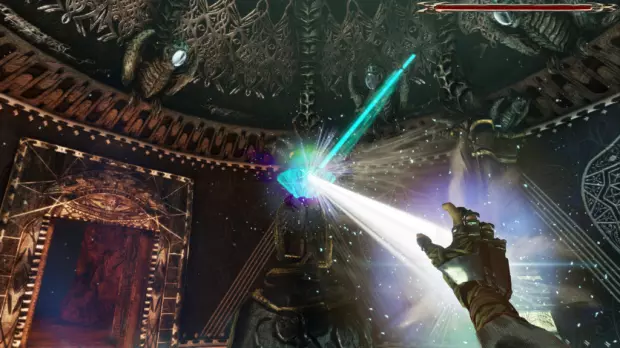
\includegraphics[width=0.5\textwidth]{verbis-virtus.png}
  \end{center}
  \caption{A screenshot of \textit{In Verbis Virtus}, where the player is casting a spell. Image taken from the Indiegogo web page \cite{RefWorks:134}.}
\end{wrapfigure}

\textit{In Verbis Virtus} is an independent 3D fantasy adventure game developed by Indomitus Games for Windows \cite{RefWorks:22}. It requires the player to solve puzzles in a 3D environment and battle enemies using magic.
\\
\\
When a microphone is connected, the player is able to cast spells using their voice by saying specific phrases defined by the game. For example, to cast a spell that produces a floating light source to brighten a room, a user must say, ``let there be light'', or if the user wishes to shoot an energy beam from their hand, they must say, ``Beam of Light'', and so. These phrases appear to be hard-coded into the game.
\\
\\
There are several limitations with this implementation of voice control. Firstly, since the phrases are hard-coded, there is no lenience in variations of the phrases, e.g. ``create a light'' or ``Laser of Light'', etc. This can seem mundane and no different to a user pressing the same button repeatedly to cast a spell.
\\
\\
Another limitation is that the user is still required to use a keyboard and mouse to perform other actions in the game, such as moving around, looking around, and navigating menus and message boxes. The voice control interface cannot be used to perform these actions. The voice control interface itself does not seem integral to the experience, as the user could just simply press a key that performs the spell instead of saying the same phrase over and over again.
\\
\\
This voice recognition interface could be improved by allowing the player to perform any action within the game using their voice, as well as allowing for more variation in what the user can say for each action.

\newpage
\subsubsection{Skyrim with Kinect}

\begin{wrapfigure}{R}{0.5\textwidth}
  \begin{center}
    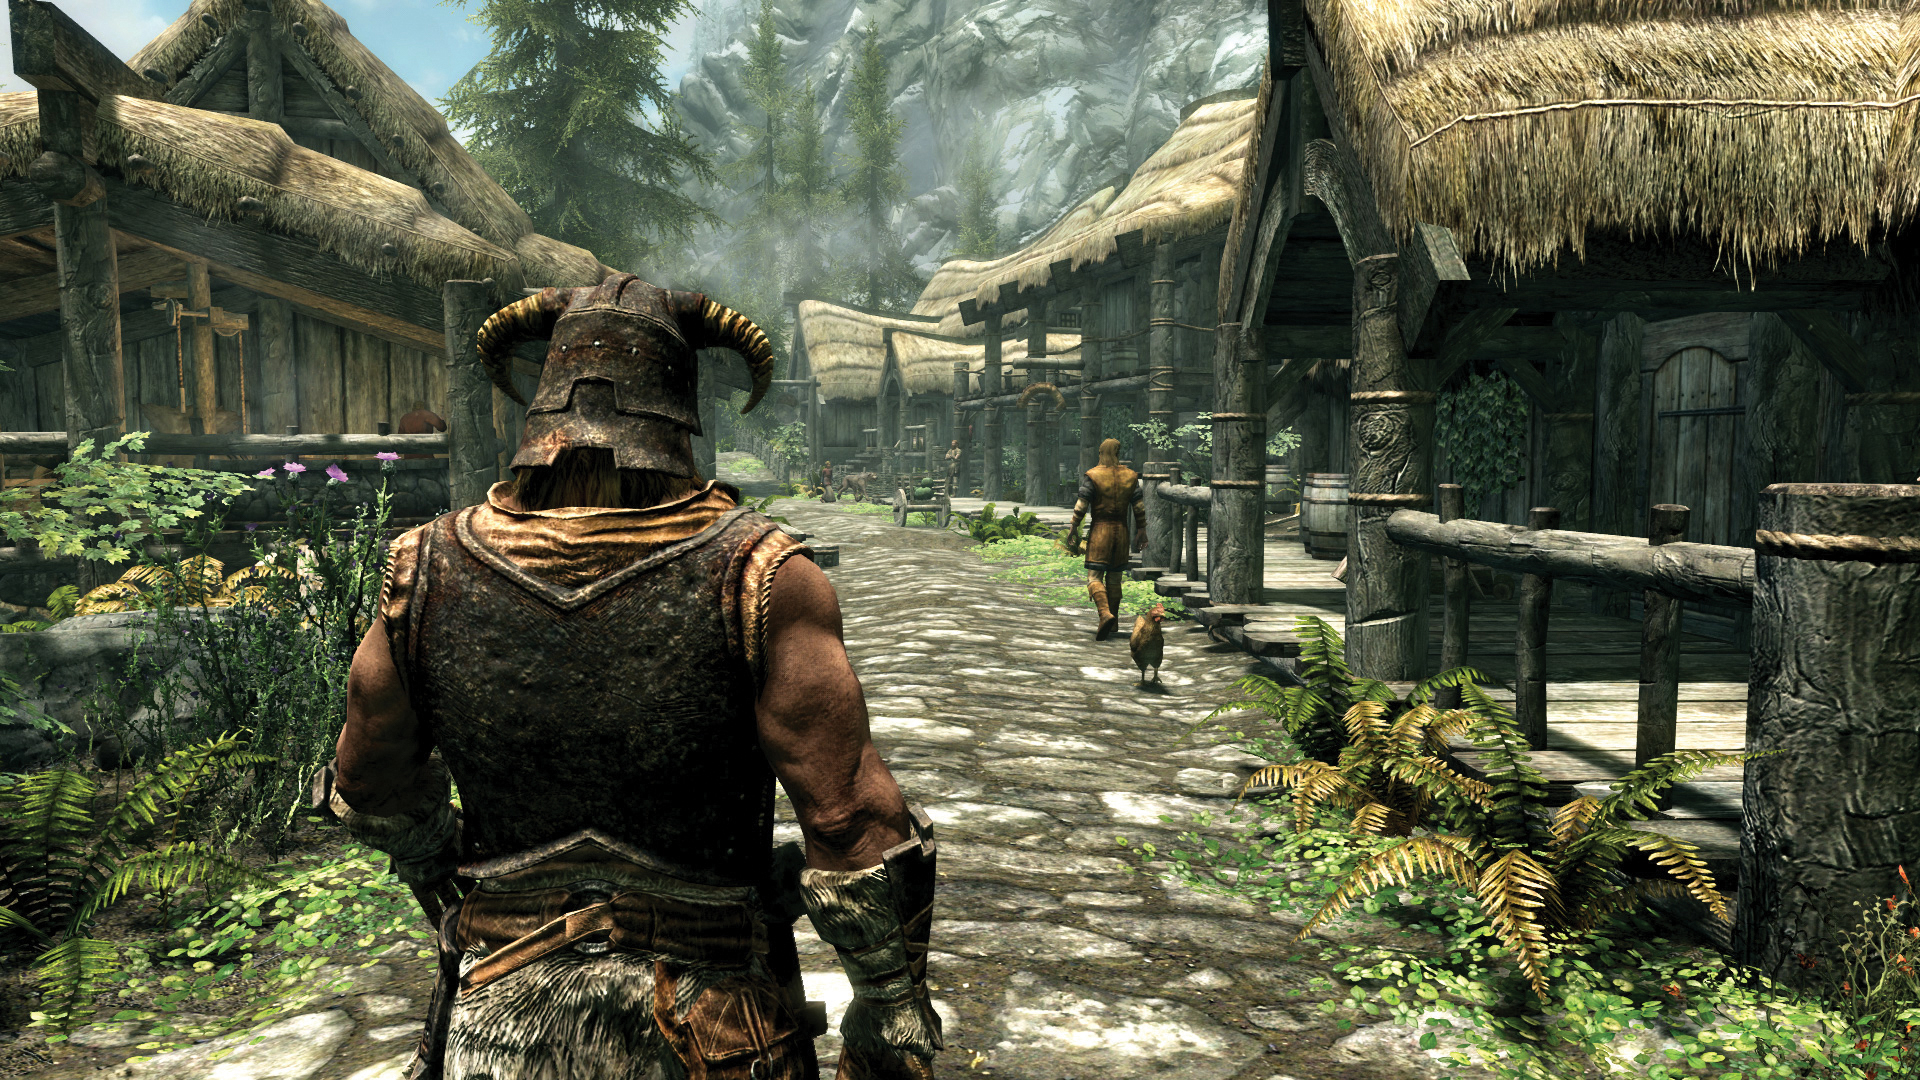
\includegraphics[width=0.5\textwidth]{skyrim-overview-media--riverwood.jpg}
  \end{center}
  \caption{A screenshot from \textit{The Elders Scrolls \rom{5}: Skyrim}. Image taken from the game's official web page \cite{RefWorks:23}.}
\end{wrapfigure}

\textit{The Elders Scrolls \rom{5}: Skyrim} is a first-person action role-playing game developed by Bethesda \cite{RefWorks:23}. The Xbox 360 version of the game supports the Microsoft Kinect peripheral which allows the player to execute voice commands \cite{RefWorks:24}. The user can use over 200 hundred pre-configured voice commands, and these can be used simultaneously with the traditional control scheme.
\\
\\
There are voice commands available that allow the user to navigate the game's menu screens. For instance, the player would say, ``quick items'' to open their inventory menu. Afterwards, the user can open menus for specific categories of items such as ``potions'', ``books'', etc. However, it doesn't seem to be possible to use any of the items selected from the menu within the game using only a voice command; this is only possible if you assign the item to a `hotkey' (e.g. by saying, ``assign health potion'' once you have highlighted a potion item), and then saying ``equip health potion'' during the game. See the Appendix \ref{appendix:skyrim} for a full list of available voice commands.
\begin{center}
\begin{figure}[H]
  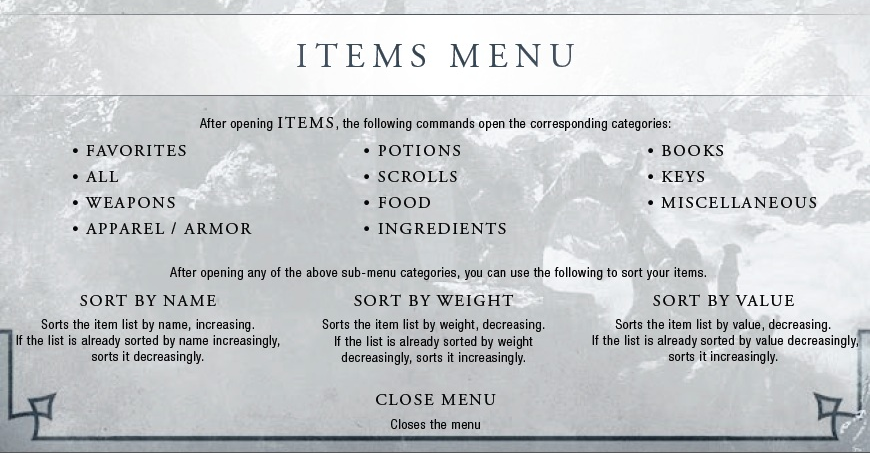
\includegraphics[width=\textwidth]{skyrim-item-commands.png}
  \caption{Voice commands that are available within the items menu in Skyrim.}
\end{figure}
\end{center}
This system, despite being optional to the player, helps to reduce the time spent searching through the menu screens. However, it appears that this system also hard-codes the phrases that can be said by the player with no flexibility in how the player can say the command.

\subsubsection{Star Trek: Bridge Crew}

\begin{wrapfigure}{R}{0.5\textwidth}
  \begin{center}
    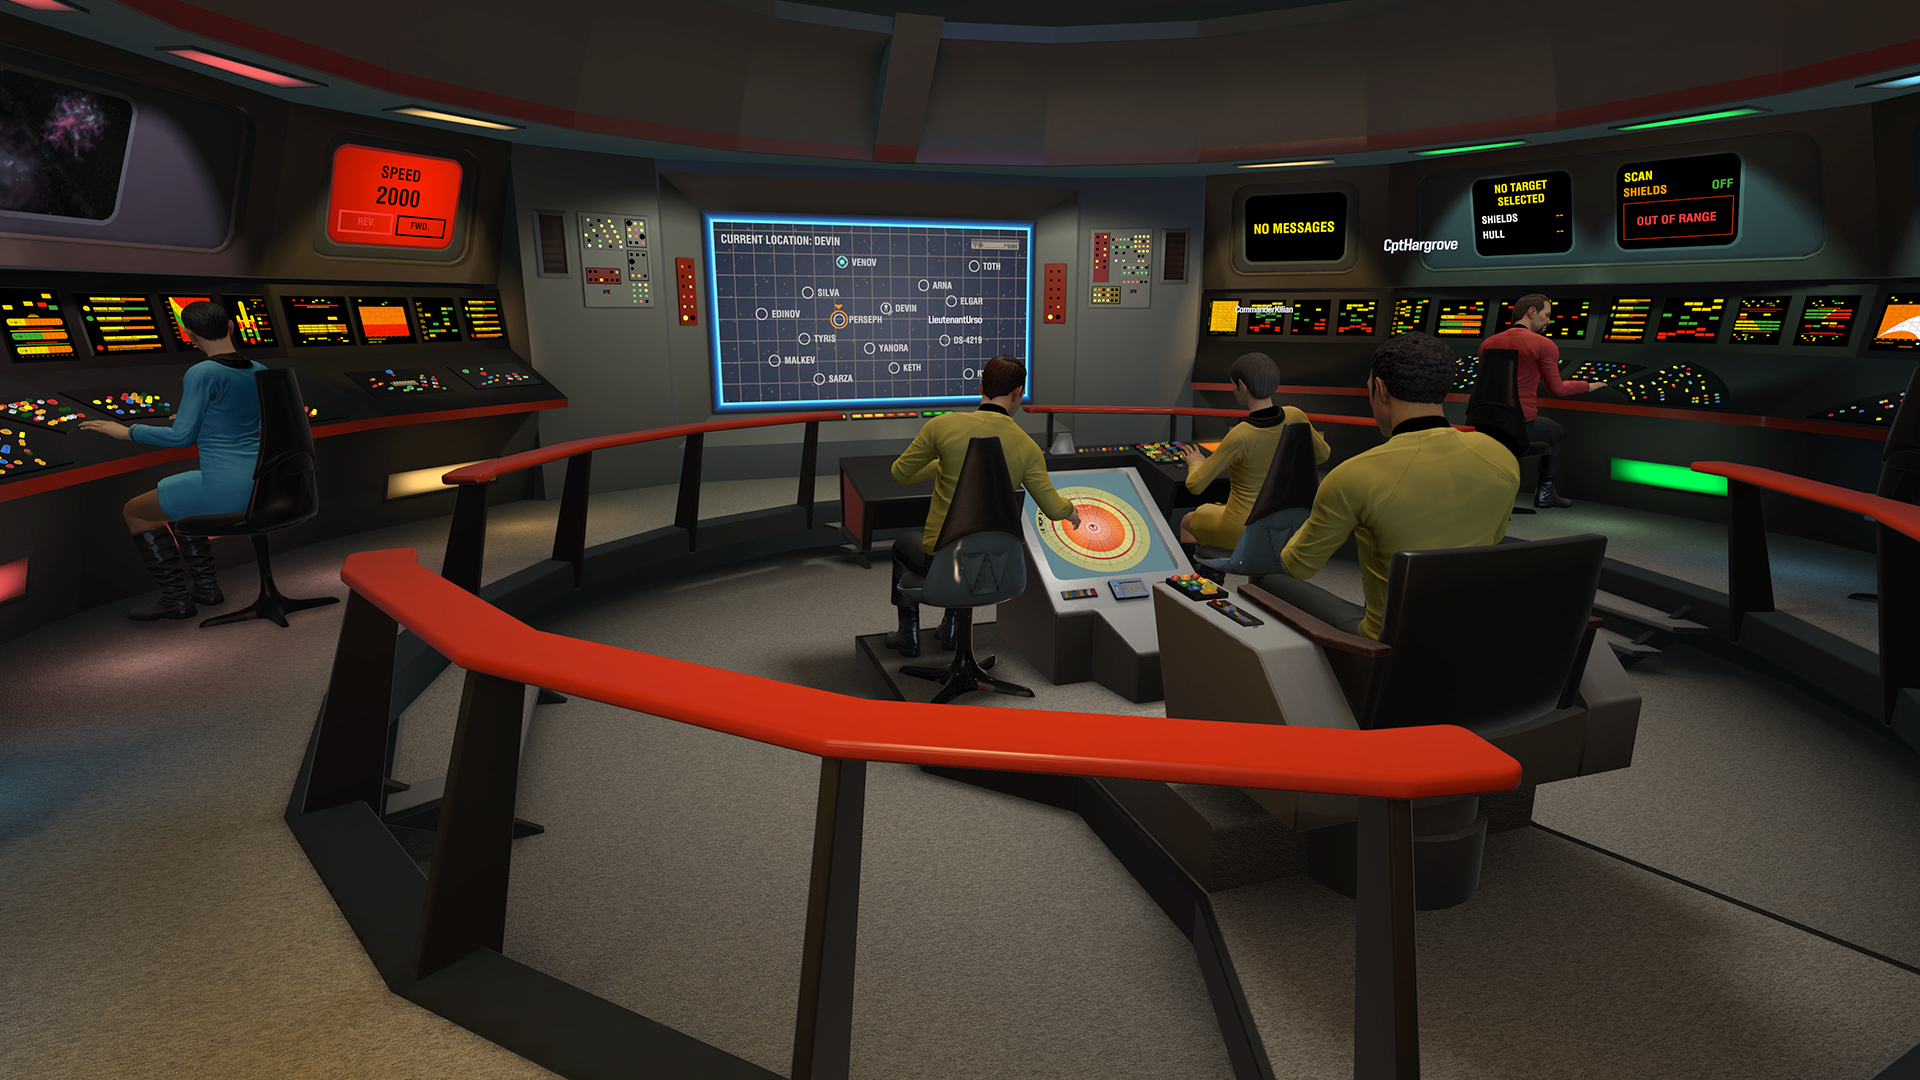
\includegraphics[width=0.5\textwidth]{star-trek.jpg}
  \end{center}
  \caption{A screenshot of \textit{Star Trek: Bridge Crew}. Image taken from the Steam web page \cite{RefWorks:135}.}
\end{wrapfigure}

\textit{Star Trek: Bridge Crew} is a virtual reality game developed by Ubisoft. This game allows the player to issue voice commands to AI crew members on a spaceship \cite{RefWorks:29}. In order to develop a more interactive and realistic experience, the development team used IBM Watson's interactive speech capabilities.
\\
\\
The API allows commands to be delivered in a variety of ways, as the speech is parsed for its meaning using Watson's Conversation service. For example, a player could say, ``show me the ship's status report'', or they could say it in a different way such as, ``damage report'' to execute the same command \cite{RefWorks:25}. This provides the user with more freedom in how they convey their request to the AI, giving the player a ``new level of sense of presence'' \cite{RefWorks:26}. See Section \ref{section:watson} for more details on IBM's Watson API.
\\
\\
The voice recognition design used in this game is similar to the proposed design outlined in this report. The user's intent should be extracted from the phrase that they speak, so similar phrases should map to the same intent. Unfortunately, Watson's API is a paid cloud service; so the game requires a constant internet connection to play.

\subsubsection{Classic Zork on Alexa}

\textit{Zork} is a trilogy of classic text-based role-playing games that support a free-form style of input (e.g. in a terminal). The player is provided with an input scenario (e.g. ``You are standing in an open field west of a white house, with a boarded front door. There is a small mailbox here.''), and the user types commands that they want to execute (e.g. ``open mailbox'' or ``attack troll with sword'') \cite{RefWorks:35}. The exploration part of the proposed game in this report will be loosely based off Zork's exploration mechanics of interacting with objects in the surroundings.
\\
\\
To add voice control to Zork, these commands could be delivered using a speech-to-text interface. A group of developers created a port of Zork running on Amazon's Alexa Skills Kit \cite{RefWorks:37}. This allows the player to deliver commands using their voice as if they were typing the phrases into a terminal. However, this implementation still suffers from the limitations of Zork's free-form input.

\subsection{Limitations of Zork}

The exploration mechanics of the proposed design in this report will be based on Zork's general gameplay of interacting with objects in the environment to solve puzzles, and the limitations of Zork's free-form input are discussed here.
\\
\\
Zork supports a number of text commands, which usually take the form of a verb-noun structure, such as ``use $<$noun$>$'' or ``take $<$noun$>$'', but it also supports some more sophisticated commands with complex structures, such as ``give all but the pencil to the nymph'' or ``drop all except the dart gun'' \cite{RefWorks:36}.
\\
\\
Zork's free-form input still has some limitations. For example, it still cannot accept all variations of specific intents. For instance, below is a list of accepted and rejected commands if the user wishes to open a mailbox in front of them:
\begin{itemize}
	\item ``open mailbox'' | \textcolor{ForestGreen}{Accepted}
	\item ``open the small mailbox'' | \textcolor{ForestGreen}{Accepted}
	\item ``can i open the mailbox'' | \textcolor{red}{Rejected}
	\item ``check the mailbox'' | \textcolor{red}{Rejected}
	\item ``find out what's in the mailbox'' | \textcolor{red}{Rejected}
\end{itemize}
Below is a list of results for closing the mailbox:
\begin{itemize}
	\item ``close mailbox'' | \textcolor{ForestGreen}{Accepted}
	\item ``shut mailbox'' | \textcolor{red}{Rejected}
	\item ``close the letterbox'' | \textcolor{red}{Rejected}
	\item ``close the red mailbox'' |\textcolor{red}{ Rejected}
	\item ``close the postbox'' |\textcolor{red}{ Rejected}
\end{itemize}
The rejected text commands could be valid phrases that express an intent to open some sort of mailbox. Zork has a pre-defined list of verbs and sentence structures that it can accept, and sticks to those without much flexibility.
\\
\\
Since most of the supported commands take the form of a verb-noun structure, this could be used in the proposed design as the general structure of commands expected by the user.

\subsection{Voice Recognition Implementations}

There are many tools and services available that allow developers and users to add voice recognition to video games, with some discussed here:

\subsubsection{Tazti - Speech Recognition for PC Games}

\textit{Tazti} is a keyboard mapping tool available to players to be used with any type of PC game that uses the keyboard \cite{RefWorks:28}. The user sets up a profile for each game separately by mapping speech commands to one or more keys. For instance, the user could say ``fire'' or ``shoot fire'' and this would map to the keystrokes required to cast a fire spell.
\\
\\
While this tool is not directly integrated into games by the developer, it has the advantage of being able to work with almost any PC game that uses a keyboard, such as role-playing games, first-person shooter games, and action games. However, the voice commands are limited to being hard-coded, so there is no way of varying the speech commands slightly, even if the meaning is the same. It is also not freely available and a license needs to be purchased.

\subsubsection{PocketSphinx for Unreal Engine 4}

\textit{Sphinx-UE4} is a speech recognition plugin for the game engine, Unreal Engine 4 \cite{RefWorks:104}, based on the PocketSphinx library which provides offline speech-to-text \cite{RefWorks:105}. The plugin allows the developer to specify keywords and the commands that they map to (e.g. ``turn right'', ``enable sprint'', ``kick the ball'', etc).
\\
\\
The plugin also supports grammar files. A grammar contains the grammatical structure that an accepted input can take, such as, \texttt{<digit> <operation> <digit>}. This will accept input such as, ``three add five'', ``six minus four'', ``two times twelve'', and so on.

\subsubsection{Houndify}
\label{section:houndify}

\textit{Houndify} is a paid cloud service developed by SoundHound that allows developers to add voice recognition and control to any application they wish \cite{RefWorks:30}. The API takes as input either a text string or audio samples and returns a JSON string containing the response to the input. This response can range from anything: from home automation control, to weather updates, and more. The response would be in the form of an intent - a single word representing the action to be executed. For example, any attacking phrase would map to an intent called, ``ATTACK''.
\\
\\
As well as having built-in voice commands already for specific domains (such as all weather commands or sports update commands), Houndify also supports the creation of custom voice commands by the developer. To create a custom command, the expression to be said by the user is specified using a syntax similar to regular expressions, but instead specifies the general phrase structure, and the expression is mapped to an intent \cite{RefWorks:33}.
\\
\\
Below is an example of a possible expression for attacking a troll:
\begin{center}
``attack'' . ``troll''
\end{center}
Here, the player would have to say, ``attack troll" to execute the intent. This can be expanded to have more variation in how the user can say this command:
\begin{center}
(``attack" $\vert$ ``hit") . [``the"] . ``troll"
\end{center}
Here, the player can say phrases such as, ``attack the troll" or ``hit troll". The expression can be further expanded. However, the expression will eventually become long and confusing:
\begin{center}
(``attack" $\vert$ ``hit" $\vert$ ``damage") . [``the"] . [``big" $\vert$ ``large"] . ``troll" . [(``with" $\vert$ ``using") . [``a"] . (``sword" $\vert$ ``hammer" $\vert$ ``axe")]
\end{center}
Even though this expression allows for more variation in what the user can say, it still doesn't cover all the possible variations of specifying an attack, and this long expression is only for one intent; many more expressions would have to be written for other intents, and this can become tedious for the developer.
\\
\\
While this API would be useful for building a personal assistant similar to Apple's Siri or Amazon's Alexa, it does not seem feasible for this project due to the time required to write the expressions for different commands. This is also a paid service, so users are charged for each query they make. It also requires a constant Internet connection to use.

\subsubsection{Watson Conversation Engine}
\label{section:watson}

IBM's Watson API features a Conversation service that allows developers to build voice recognition interfaces that understand natural language input \cite{RefWorks:27}. The developer defines the training data to be used by the API (in order to train a natural language classifier) using `intents' and `entities' \cite{RefWorks:31}.
\\
\\
`Intents' are the goals that a user will have as they interact with the application. For example, in a voice-controlled car, an intent could be \texttt{wipers\textunderscore on}, in order to activate the windscreen wipers. This intent would be paired with example utterances in the form of text strings, such as ``turn on the wipers", ``switch on the windscreen wipers", and so on. The more examples given, the more accurate the trained model will be.
\begin{center}
\begin{figure}[H]
  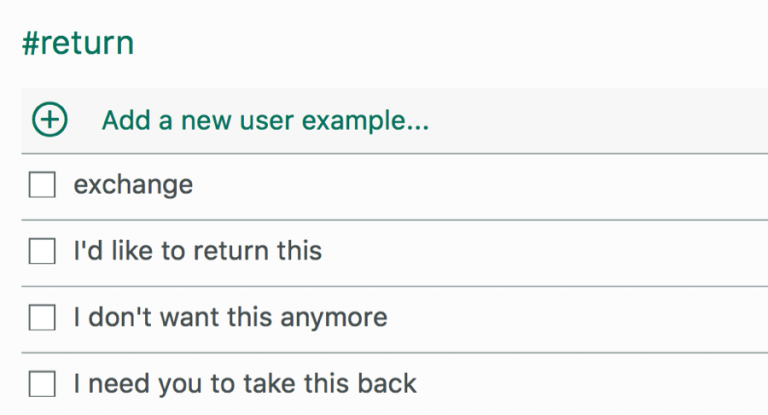
\includegraphics[width=\textwidth]{intent-return.png}
  \caption{An example of an intent to return something, along with examples of phrases for the intent. Image re-used from an IBM blog post \cite{RefWorks:34}.}
\end{figure}
\end{center}
`Entities' are classes of objects that help to provide context to intents. For example, with the \texttt{wipers\_on} commands above, it is not clear whether the user is referring to the wipers on the front of the car or the wipers on the back of the car (the API will assume the front by default). If the entity is included in the phrase spoken by the user, then the context of the intent becomes clear.
\begin{center}
\begin{figure}[H]
  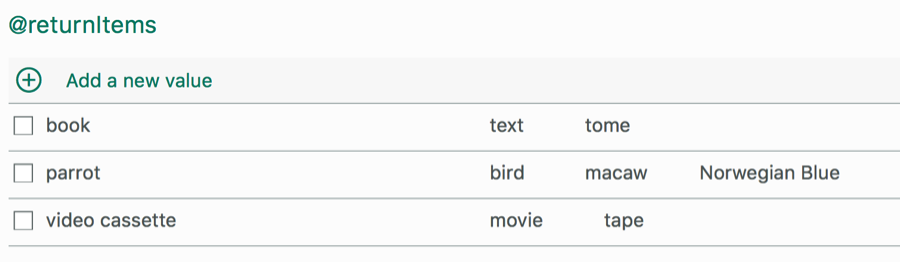
\includegraphics[width=\textwidth]{returnitems.png}
  \caption{An example of entities for items that can be returned. Entities that have been grouped together (usually synonyms) are placed on the same row \cite{RefWorks:34}.}
\end{figure}
\end{center}
Once the classifier is trained, it will be able to use the examples of intents provided to classify whether new examples of phrases have the same meaning as those. For example, if the user says, ``activate the windscreen wipers at the front of the car", the classifier will return the \texttt{wipers\textunderscore on} intent, even though this input is very different in structure to the examples provided above. A demo is available to test this in a web browser \cite{RefWorks:32}.
\\
\\
According to a research paper by McCord, Murdok and Boguraev on \textit{Deep Parsing in Watson} \cite{RefWorks:112}, the engine consists of two deep parsing components: an English Slot Grammar (ESG) parser and a predicate-argument structure (PAS) builder. These allow Watson to produce parse trees of a sentence and extract pattern-based relations from it, such as question decomposition, hypothesis generation, and evidence scoring.
\\
\\
This API is very flexible and matches the first objective of this project; only a few examples of possible inputs need to be provided for each intent, and then the classifier can infer whether any new input strings will match the same intent. Unfortunately, despite being a very powerful system, this still remains a paid cloud service, so users are charged for each API request. It also requires a lot of processing power (which is offloaded to a cloud server) for the many machine learning algorithms being used here. However, a simpler system may possibly be implemented that uses a similar concept to the intents and entities framework, and the proposed design in this report uses a similar concept that runs locally.
\\
\\
There is a similar API called DialogFlow \cite{RefWorks:106}, which works very similarly to IBM's Watson Conversation engine. However, it suffers from the same issues as above (e.g. cloud-based, pay-per-request, etc).

\subsection{Natural Language Processing}

Natural Language Processing (NLP) forms a major component of this project. This will give the developer the ability to take an arbitrary string of text and infer its meaning, and map it to an intent. Below are some explanations on NLP concepts related to this project.

\subsubsection{Stages of Natural Language Processing}

\begin{center}
\begin{figure}[H]
  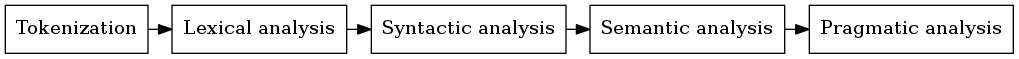
\includegraphics[width=\textwidth]{nlp-stages.png}
  \caption{The general stages of processing a text string for its meaning using NLP.}
\end{figure}
\end{center}

NLP can be broken down into six stages \cite{RefWorks:38}. The first stage is the tokenization, where a raw text string is broken down into words (usually separated by spaces).
\\
\\
The second stage is the lexical analysis, where the output of the tokenization process is improved upon by looking at words that can be taken apart even further (or rejoined if needed) to uncover more information. These include words such as: clictic contractions (e.g. ``what're" would tokenise to ``what" and ``are",. while ``we're" would break down to ``we" and ``are"); end-of-line hyphens that split whole words into parts when using a justification alignment; and shortened titles or abbreviations (e.g. Dr., U.S.A., etc.) \cite{RefWorks:39}.
\\
\\
The third stage is syntactic parsing, where the grammatical structure of the sentence is determined. This is usually achieved by generating a syntax tree of each sentence, where each word is broken down into a terminal from a given grammar (e.g. verbs, nouns, adjectives, determiners, etc.) \cite{RefWorks:40}.

\begin{center}
\begin{figure}[H]
\begin{center}
  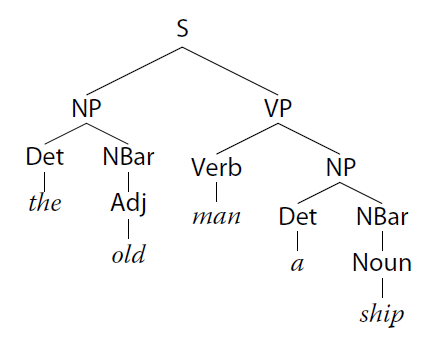
\includegraphics[scale=1]{syntax-tree.png}
  \caption{An example of a syntax tree for the sentence, ``the old man a ship". Diagram taken from the Handbook of Natural Language Processing  \cite{RefWorks:40}.}
  \label{fig:old-man}
  \end{center}
\end{figure}
\end{center}

In the example in Figure \ref{fig:old-man} for the sentence, ``the old man a ship", the word, ``man" could be mistaken to be a noun, but in this case, the sentence is implying that the elderly control a ship, and therefore, ``man" is actually a verb here. This meaning can be more easily inferred when the sentence is broken down using a syntax tree, as above.
\\
\\
The final two stages are very similar and is difficult to separate them into separate stages. Both stages involve determining the meaning of the sentence. The fourth stage is often concerned with semantic analysis, whereas the last stage is more concerned with discourse analysis \cite{RefWorks:39}.

\subsubsection{Part-of-Speech Tagging}

A technique often used in NLP is to try to label each word with its correct part of speech, known as part-of-speech (POS) tagging. POS-tagging systems generally use a tagset containing POS tags to assign a tag to each word. The most popular tagset is the Penn Treebank tagset. This consists of 48 tags, of which 12 are for punctuation and other symbols \cite{RefWorks:41}. See the Appendix \ref{appendix:penn} for the full Penn Treebank tagset.
\\
\\
There are two main challenges regarding POS tagging. The first challenge is that words can sometime be ambiguous. That is, the word can be assigned a number of possible POS tags depending on its context. For instance, the word, ``can" can either be a verb (``I can..."), a noun (``a can of tuna"), or another verb with a completely different meaning (``can that noise!") \cite{RefWorks:43}. The many meanings that are attributed to a word are known as its \textit{word senses}.
\\
\\
The second challenge involves words that are unknown to the tagger and cannot be tagged. A default tag is required for words which are unknown, but that could interfere with the rest of the POS-tagging process \cite{RefWorks:41}.
\\
\\
The proposed design for this project will use an open-source POS tagger in order to identify specific words in the player's input, namely verbs and nouns.

\subsubsection{Slot Filling}

According to the authors of \textit{Speech and Language Processing} \cite{RefWorks:107}, three tasks need to be done to understand a user's utterance. The first is \textit{domain classification}, to determine the topic that the user is talking about (e.g. weather, sport, etc), although this is unnecessary for single-domain applications such as the contents of a video game. The second task is \textit{intent determination}, to determine the goal of the user, and finally, the last task is to do \textit{slot filling}.
\\
\\
Slot filling involves determining the specific details of an intent by defining a grammar that the intent must adhere to. An example for arithmetic operations would be, \texttt{<DIGIT1> <OPERATION> <DIGIT2>}. The input would be parsed by a context-free grammar parsing algorithm to extract each bit of information in order to fill each slot in the grammar. Figure \ref{fig:slot-filling-diagram-example} shows an example of a slot-filling grammar.
\\
\\
A disadvantage to slot-filling using context-free grammar parsing is that not all valid expressions for an intent would match with the slots. A solution to this would be to define multiple grammars for different structures of inputs.

\begin{center}
\begin{figure}[H]
\begin{center}
  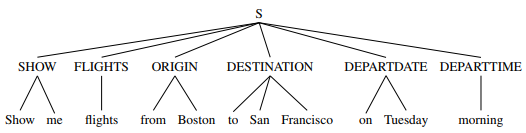
\includegraphics[scale=1]{slot-filling.png}
  \caption{An example of a slot-filling grammar for flights, using slot names as the internal parse tree nodes. Diagram taken from Chapter 29 of the book, \textit{Speech and Language Processing} \cite{RefWorks:107}.}
  \label{fig:slot-filling-diagram-example}
  \end{center}
\end{figure}
\end{center}


\subsubsection{Synonyms and Hypernyms}

\textit{Synonyms} are words or phrases which have a similar meaning to another word  \cite{RefWorks:44}. For example, the word ``dog" has seven word senses (i.e. different meanings), and for one of the word senses with a meaning of, ``a member of the genus Canis", the synonyms would be, ``domestic dog" and ``Canis familiris" \cite{RefWorks:45}.
\\
\\
A \textit{hypernym}, on the other hand, is a word or phrase which generalises words for which it is a hypernym of. For instance, the word, ``instrument" is a hypernym of ``guitar", because a guitar is a type of instrument. Similarly, the word ``animal" is a hypernym of ``cat" (or, at least, the sense which refers to the domestic animal, as ``cat" can have several usages).
\\
\\
The synonyms and hypernyms of words and phrases can be represented as a hyper-tree structure, where the parent nodes are hypernyms of the child nodes, while each sibling node would represent a different word sense for a word, with each sibling containing the synonyms for that sense.

\begin{center}
\begin{figure}[H]
\begin{center}
  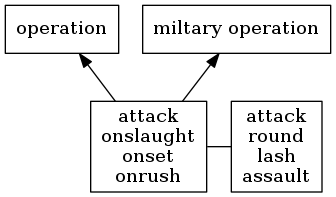
\includegraphics[scale=1]{hypernym-tree.png}
  \caption{A partial hypernym tree showing the synonyms and hypernyms for one of the senses of the noun, ``attack". The ``attack" verb sense (right) is a sibling node.}
  \end{center}
\end{figure}
\end{center}

Synonyms and hypernyms could be used to determine the semantic similarity between words and infer whether the user's intent matches a certain action.
\\
\\
Note that a \textit{hyponym} is the inverse of a hypernym (e.g. the word, ``cat" is a hyponym of ``animal").

\subsubsection{Semantic Similarity}
\label{section:bg-semantic-sim}

There are many ways of calculating the semantic similarity between two words or phrases. Many of these methods use the synonym and hypernym trees of the words to infer similarity, and assign a `similarity score' to them. This score could be used to determine whether, for instance, a verb has semantic similarities to one of the actions in a game, and therefore can be mapped to that action.
\\
\\
The following are some examples of measures for semantic similarity \cite{RefWorks:46}. The first is the Wu and Palmer (WUP) measure, which takes the depth in the hypernym tree of the Least Common Subsumer (LCS) (that is, the first hypernym that both words have in common) and compares it with the sum of the depths of each word. The formula for the similarity of words $w_1$ and $w_2$ is as follows:

$$sim_{wup} = \frac{2*depth(LCS(w_1,w_2))}{depth(w_1)+depth(w_2)}$$

For example, the WUP score for the semantic similarity between ``juice" and ``water" is calculated as follows \cite{RefWorks:49}:

\begin{lstlisting}[frame=single]
T1 = HypernymTree( juice ) =
    [Sense #1] *ROOT* < entity < physical_entity < matter
    	< substance < food < foodstuff < juice

T2 = HypernymTree( water ) =
    [Sense #3] *ROOT* < entity < physical_entity < matter
    	< substance < food < water

Lowest Common Subsumer(s) = argmax(depth(subsumer(T1,T2)))
    = { subsumer(T1[1], T2[3]) } = { food }

DepthLCS = depth( food ) = 6
Depth1 = min(depth( {tree in T1 | tree contains LCS } )) = 8
Depth2 = min(depth( {tree in T2 | tree contains LCS } )) = 7
Score = 2 * DepthLCS / ( Depth1 + Depth2 ) = 2 * 6 / (8 + 7)
Score = 0.8
\end{lstlisting}

The WUP score of 0.8 out of 1.0 indicates that juice and water are semantically very similar \cite{RefWorks:47}, whereas the words ``chair" and ``biology" only have a WUP score of 0.17, suggesting they are not semantically similar.
\\
\\
Another measure of semantic similarity is Leacock and Chodorow's method, which relies on the shortest distance between the two words in the hypernym tree, divided by the maximum depth of the whole tree; the shorter the distance, the more similar the words are \cite{RefWorks:46}. There are many more different measures and it is possible to combine them to produce an overall score for semantic similarity.

\subsection{WordNet}

Princeton University created a large lexical database for the English language, called \textit{WordNet} \cite{RefWorks:20}. Words are grouped into synonyms (known as synonym sets, or \textit{synsets} for short), and are connected to their respective hypernyms (more general words) and hyponyms (more specific words), creating the large hypernym tree mentioned previously. The database is open-source and is used extensively in this project, using various APIs that interact with the WordNet database (which will be initially downloaded by the game for offline use).

\subsection{Generating Objects from Descriptions}

One feature for the proposed design of the RPG is to prevent the developer from manually placing objects in a room/environment within the game. A designer may want to just provide a description of the room without having to program anything. A simple solution to this would be to perform noun extraction on the description to extract the objects that should be in the room. However, it would also be useful to extract relations of objects to other objects as well. For instance, a lamp should only be on a table if the table exists in the room; if the table is removed/broken by the player, then the lamp should now be on the floor. This would allow for more information to be extracted about the objects in the room, as opposed to simply their existence.
\\
\\
Fader, Soderland and Etzioni from the University of Washington proposed a solution for extracting these types of binary classifications using an extraction algorithm which takes as input a POS-tagged input and returns a set of triples representing binary relationships. They created a tool for this called \textit{ReVerb} \cite{ReVerb2011}. Taking the sentence, ``A knife is on the floor", it would extract the triple, \texttt{(a knife, be on, the floor)}, representing the binary relationship (``be on") between the knife and the floor. Using this, more interesting room generation may be possible just from a user-given description of the room.

\subsection{Generating Descriptions from Objects}

The opposite to the above is to be able to generate text-based descriptions of the current situation that the player is in based on objects around them. For instance, a description could be, ``You are in a room lit by a candle on a table. There is a piece of broken glass on the floor and a door in front of you." One could hard-code this sentence for each room the player visits, but if there are a lot of rooms in the game, this could become time-consuming. Developers would like to generate a description of the current situation based on sparse pieces of information (such as the items in the room, plus their locations, in a vector representation). This is the opposite of the above, where the object of a sentence/phrase is extracted; developers may want to go in the opposite direction.
\\
\\
This is a relatively new field in NLP as it is particularly difficult. One method of sentence generation is suggested by Iyyer et al \cite{RefWorks:55}, where recursive autoencoders (a type of neural network) are used to generate a decomposition model of the sentence that can be used to reconstruct the sentence again. However, they found that proper nouns were not reconstructed correctly, and the model would need to be built in the first place to reconstruct the sentence.
\\
\\
Another group of researchers proposed a method of sentence generation which involves taking a sum of word embedding vectors and modelling it as a mixed integer programming problem \cite{RefWorks:54}. However, this also requires the original sentence to be de-constructed in the first place in order to know what the vector should contain.
\\
\\
One possible solution would be to only hard-code the general sentence structure of the description of rooms, and then insert the appropriate adjectives and nouns of the items, which is given as input in the form of a vector of strings.

\subsection{Object Properties}

One issue to note is when a user attempts to specify an item based on a description of it (e.g. the user says, ``attack the enemy with a sharp object"); players would like to be able to select an item that matches the description (e.g. a sword is sharp, so it will be chosen if the user possesses one). One approach to this is to assign the items a set of properties such as whether it is sharp or blunt, whether it can be thrown, and so on.
\\
\\
A similar technique was used by the developers of Scribblenauts for the Nintendo DS. Using the company's ObjectNaut engine, the game utilises a large database of a hierarchy of objects \cite{RefWorks:48}. This allows them to design sprites for different objects (such as a cyborg, robot or android), but assign them the same interaction properties. However, this still required the developers to go through encyclopaedias word-by-word to find which ones had similar properties. Using the semantic similarity scoring mechanism, this would not need to be done, as it can be inferred whether an object has a certain property based on how semantically similar it is to that property (e.g. an object may be sharp if it is semantically similar to the word, "sharp"), instead of hard-coding each property for every object in the game.
\\
\\
By assigning items different properties, the actions that the user can perform for each variation of items (e.g. sword, katana, knife, etc.) does not need to be hard-coded. Instead, there can be general objects which have certain properties, and then the actions for each general object can be coded. For example, there could be a general object with a `sharpness' property, that would be able to cut things, and all swords and knifes would be of this type of general object, and therefore also considered sharp.
\newpage

\section{Design}
\subsection{Target Platform}

According to Ovum's Mobile Games Market forecast for 2017-2022 \cite{RefWorks:109}, mobile games continue to increase their market share as they grow in popularity, and within the next two years, almost half of the total video game revenue generated will come from mobile games. Therefore, it makes sense to design a system for a mobile platform such as iOS or Android.  It also allows for hands-free input as a future extension.
\\
\\
The chosen platform to develop the voice recognition system and game will be Android mobile devices, as the availability of the open-source Google Speech-to-Text API means that less effort is required to transform the user's utterance into text.

\subsection{Java Programming Language}

The language used to develop the application is Java, which is an object-oriented programming (OOP) language. The use of an OOP language makes it easier to create objects in a video game using the inheritance hierarchy. For example, there would be an abstract class for physical objects called \texttt{PhysicalObject}, and another class such as \texttt{Glass} would be a derived class of a \texttt{PhysicalObject}, and so on.
\\
\\
A disadvantage to using Java is that it does not support multiple inheritance, unlike other languages with OOP constructs such as C++, due to methods such as \texttt{super()} having the same signature for all parent classes. For instance, a \texttt{Glass} class cannot inherit properties from both a \texttt{PhysicalObject} and a \texttt{BreakableObject} (i.e. they are both direct parents of the \texttt{Glass} class). Instead, this must be overcome by making the inheritance a single chain (e.g. \texttt{Glass} inherits from \texttt{BreakableObject} which inherits from \texttt{PhysicalObject}). While this can be considered a hindrance in some circumstances, it is not a major issue for the proposed design of the game.
\\
\\
While Java applications | and therefore Android | support the invocation of native code such as C++ using the Java Native Interface (JNI) for improved performance, this will not be used due to time constraints for the project.

\subsection{System Overview}

The following is a brief description of the voice recognition system, including the main components and the general flow of data.
\\
\\
The voice recognition system takes as input the raw microphone input containing the player's utterance, and outputs a response as a string, with the side-effect being the execution of a developer-defined action based on the player's utterance. Figure \ref{fig:flow-chart} shows a simple flow chart outlining the main stages of the voice recognition system from input to output.

\begin{center}
\begin{figure}[H]
\begin{center}
  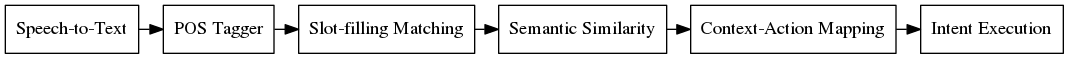
\includegraphics[width=\linewidth]{flow-chart.png}
  \caption{A flow chart showing the general stages of the voice recognition system. Graph generated using Graphviz.}
  \label{fig:flow-chart}
  \end{center}
\end{figure}
\end{center}

The steps are briefly described here and explained in more detail below.

\begin{itemize}
\item The audio from the microphone input is processed into a text string using a Speech-to-Text (STT) engine. This string is then split up into a list of words.

\item The list of words is then used to generate a list of Part-of-Speech (POS) tags. Each word in the list is passed to the POS tagger and added to the tag list.

\item The word list is parsed using a slot-filling grammar, e.g. "\texttt{<ACTION> <TARGET> [with] <CONTEXT>}", or "\texttt{[use] <CONTEXT> [to] <ACTION> <TARGET>}".

\item When performing the matching, the current word being parsed is sent to a semantic similarity engine, and a similarity score is calculated.

\item If the player has specified an action to be done under a certain context, then the context-action mapping is consulted to find the correct method to execute. Otherwise, the default action method is chosen.

\item Finally, the in-game function is executed, and the text output is returned, with the game state updated.
\end{itemize}

\subsubsection{Speech-to-Text}

Android features a built-in speech recognition service, via its \texttt{SpeechRecognizer} class \cite{RefWorks:110}, and this is used for the speech-to-text engine. While the API's primary method of speech recognition is via remote server communication, there is an option with the Android OS settings to perform offline speech recognition instead, by downloading the language data (although this offline method has slightly less accuracy) \cite{RefWorks:111}.
\\
\\
Using this API, the player's utterance is transformed into a text string, which is then processed by the rest of the voice recognition system. Using an existing speech-to-text API means that less time is spent trying to get the player's utterance from the microphone input.
\\
\\
In terms of user interface, the application features an on-screen button containing the image of a microphone. When the user presses this button, a voice request is initiated and lasts until the user finishes uttering their input. If the user doesn't say anything, then the response times out and is cancelled.

\subsubsection{POS Tagging}

For the Part-of-Speech (POS) tagging of the input, the open-source log-linear POS Tagger provided by The Stanford Natural Language Processing Group will be used \cite{RefWorks:113}. It is a Java archive file and can easily be imported and used in an Android Java project. The API handles all the POS tagging so no time needs to be spent implementing a POS-tagging system. 
\\
\\
The library comes with two trained models. According to the software's \texttt{README} file, the first model uses a bidirectional architecture and includes training data using word shapes and distributional similarities. The second model uses a \textit{left3words} architecture (which also uses word shape features), and the tags in the output are from the Penn Treebank tagset. According to the developers, the bidirectional model is ``slightly more accurate" with a correctness score of 97.28\%, but is much slower to tag with than the \textit{left3words} model. Therefore, the \textit{left3words} model was chosen to be used in the application. (It still features a performance correctness score of 96.97\% which is not that different to the bidirectional model's performance.)
\\
\\
With the input string broken down into an list of words, each word is used as input to the POS tagger, and the word's tag (e.g. \textit{VB}, \textit{NN}, etc.) is added to a new list containing all the tags (i.e. the index of a tag is the index of its corresponding word in the other list). Both lists will be used simultaneously in other processes.

\subsubsection{Slot-filling Matching}
\label{section:slot-filling}

The next stage is to extract the important information from the input. In many applications, particularly in games, voice commands are usually given in the imperative form (such as, ``do this", ``attack that", etc.). It is assumed that the subject of the command (that is, the entity about whom the statement is made about \cite{RefWorks:114}) is always the player (or the character that the player is controlling).
\\
\\
Generally, commands will have an imperative verb (e.g. ``attack", ``grab", ``look"), optionally followed by the target entity for which the imperative verb should be applied towards, as well as an optional context entity for which the imperative verb should be applied with.
\\
\\
As an example, take the command, ``hit the rock with a spoon". Here, the word `hit' is the imperative action and it is applied to the `rock'. The `hit' action is applied using the `spoon' as the context. The target and context help to provide a clearer intent; the user could have just said, ``hit" without mentioning the target or context, and while the action to be performed is clear, it is ambiguous as to what should be hit and with what.
\\
\\
For this stage, slot-filling structures (SFS) are used to describe the grammar of the voice commands. The SFS grammar chosen is:

\begin{center}
\texttt{ACTION TARGET WITH CONTEXT}
\end{center}

Here, parts of the input will be mapped to a \textit{block} in the grammar. The \texttt{WITH} block is for words and phrases which signify that the following words represent the context to perform the action (e.g. ``...with...", ``...using...", ``...with the power of the...", and so on). Figure \ref{fig:sfs-1} shows how parts of an example command are matched to the grammar.

\begin{center}
\begin{figure}[H]
\begin{center}
  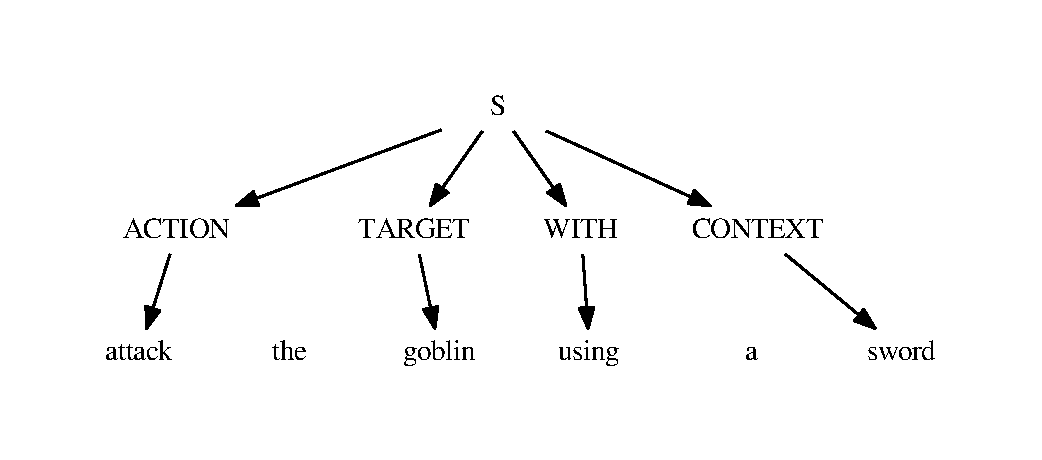
\includegraphics[width=\linewidth]{sfs-1.pdf}
  \caption{The slot-filling structure, \texttt{\{ACTION TARGET WITH CONTEXT\}} being applied to an example sentence, ``attack the goblin using a sword". Generated using Graphviz.}
  \label{fig:sfs-1}
  \end{center}
\end{figure}
\end{center}

Not all the slots have to be filled; the \texttt{TARGET}, \texttt{WITH} and \texttt{CONTEXT} blocks are completely optional to fill, but they provide more information about the user's intent. Should this information be left out, the system will fall back on the defaults for each one.
\\
\\
While this covers a large variety of commands that the user can give, such as, ``attack the troll with a sword", ``pick up the knife", or ``look around the room using binoculars", it does not cover commands that have a completely different structure. For example, the phrases, ``use a potion to heal" and ``with a key open the door" are perfectly valid commands that a user can give, but the matching blocks are in completely different order (i.e. the \texttt{CONTEXT} comes before the \texttt{ACTION}), so would not be matched with the above SFS.
\\
\\
An alternative SFS is applied when appropriate. The grammar is as follows:

\begin{center}
\texttt{WITH CONTEXT ACTION TARGET}
\end{center}

Using this slot-filling grammar, the aforementioned example commands (``use a potion to heal" and ``with a key open the door") would be accepted. Figure \ref{fig:sfs-2} shows an example of the matching.

\begin{center}
\begin{figure}[H]
\begin{center}
  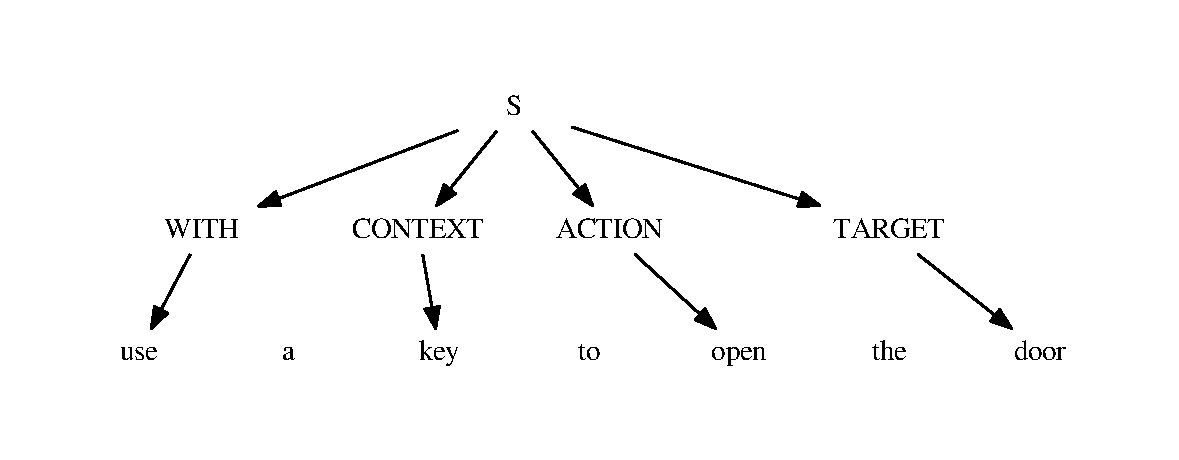
\includegraphics[width=\linewidth]{sfs-2.pdf}
  \caption{The slot-filling structure, \texttt{\{WITH CONTEXT ACTION TARGET\}} being applied to an example sentence, ``use a key to open the door".}
  \label{fig:sfs-2}
  \end{center}
\end{figure}
\end{center}

During the processing, the correct SFS will be chosen based on the structure of the phrase (i.e. by determining the relative positions of each piece of information).
\\
\\
Using lists of possible actions, targets and contexts created by the developer (specified as strings), the slot-filling process will compare the words in the input to the words in the lists in order to find a match.

\subsubsection{Semantic Similarity}
\label{semantic-sim-design}

During the slot-filling matching stage, if a word does not match any entry in the possible list of actions/targets/contexts character-by-character, then semantic similarity methods are used to determine the whether the two words are similar. For example, if the possible list of actions are, `attack', `heal' or `run', and the player's input is, ``hit'', then `hit' is similar to the `attack' action, so the `attack' action would be chosen.
\\
\\
As mentioned in Section \ref{section:bg-semantic-sim}, there are many similarity methods that have been proposed. The first method to be used in the application is the \textit{Wu and Palmer} method (WUP) described previously. Another method that is used is the \textit{Lin} method (LIN), that calculates the similarity of two words based on the information content of their least common subsumer \cite{RefWorks:46}. Information content (IC) is defined as the negative log of the probability of a concept. The probability of a concept is based on the sense frequency of a word within its synset.
\\
\\
Lin used IC to define a similarity measure similar to the Wu and Palmer method, but uses IC instead of the depths of the words in the word tree instead. The formula for the similarity of words $w_1$ and $w_2$ is as follows:

$$sim_{lin} = \frac{2*IC(LCS(w_1,w_2))}{IC(w_1)+IC(w_2)}$$

Another method used is the \textit{Lesk} method. This method determines the similarity of two words based on the overlaps in their definitions \cite{RefWorks:115}. For instance, the definition for certain senses of the words, '\textit{ash}' and '\textit{coal}' (to describe a burnt substance) have the words, `combustible', `burn' and `solid' in their definitions. Therefore, it can be deduced that the words are semantically similar. In another paper, Banerjee and Pederson extended the Lesk method by using all the definitions of all the senses for both words in the calculation, as only using one sense definition did not give enough information \cite{RefWorks:117}.
\\
\\
As well as using the definitions of the synonyms, hypernyms and hyponyms of the word, this method also uses the definitions of the word's meronyms and holonyms. Meronyms are words that represent part of something else \cite{RefWorks:121}. For example, `face' would be a meronym of `person'. Holonyms are words that represent the whole of several parts, so a `body' would be a holonym for words such as `arm', `leg' and `torso' \cite{RefWorks:121}. Using these definitions makes the Lesk method more accurate than other methods, but also adds more processing time for each calculation.
\\
\\
The WordNet database is accessed and traversed using the MIT Java WordNet Interface (JWI), which is an open-source library that interfaces with a WordNet database \cite{RefWorks:118}. A full English WordNet database is downloaded from Princeton's website, and the JWI API is loaded with it.
\\
\\
Implementations for most of the similarity methods are provided by another open-source Java library, \textit{WS4J} \cite{RefWorks:116}. While this library provides the methods for doing the calculations (such as the WUP, LIN and LESK formulas), the methods for the navigation and analysis of the WordNet database (e.g. getting hypernyms, synsets, glosses, etc.) must be implemented from scratch (see Section \ref{custom-lexical-database-impl} of the Implementation for more details).

\subsubsection{Context-Action Mapping}

Once matches have been found from the slot-filling, they are mapped to the methods that should execute that intent. If the player only specifies an action with no context, then a default action should be executed (the context itself defaults to a ``default" context type). If the player specifies a context (e.g. "...with a sword"), then a mapping is consulted to find the correct method that should be called. The different targets are handled within the method itself.
\\
\\
Table \ref{action-context-ex-table} shows an example of what a context-action `table' mapping would look like. The table is column-indexed using the action and row-indexed using the context  type. Note the \textit{null} entries which indicate that the context is not compatible with the corresponding action (for example, it does not make sense from a player to ``attack with a potion"), and the context is therefore ignored (i.e. the `default' method will execute instead).

\begin{table}[H]
\centering
\caption{An example of a developer-specified context-action mapping}
\label{action-context-ex-table}
\begin{tabular}{l|l|l|l|}
\cline{2-4}
\multicolumn{1}{c|}{\textbf{}}         & \multicolumn{3}{l|}{\textbf{actions}}                  \\ \hline
\multicolumn{1}{|l|}{\textbf{context}} & \textit{attack}    & \textit{heal}  & \textit{open}    \\ \hline
\multicolumn{1}{|l|}{\textit{default}} & AttackDefault()    & HealDefault()  & OpenDefault()    \\ \hline
\multicolumn{1}{|l|}{\textit{weapon}}  & AttackWithWeapon() & null           & null \\ \hline
\multicolumn{1}{|l|}{\textit{potion}}  & null               & HealWithPotion() & null             \\ \hline
\multicolumn{1}{|l|}{\textit{key}}     & AttackWithKey()    & null           & OpenWithKey()   \\ \hline
\end{tabular}
\end{table}

\subsubsection{Intent Execution}

Each non-null field in the context-action map contains a class that extends from an abstract class, \texttt{Action}. This abstract class contains a method called \texttt{run()}, which executes the in-game intent. This method is overridden by a derived class (such as \texttt{AttackDefault} and \texttt{HealWithPotion}). These \texttt{run()} methods act as wrappers for the methods that would execute in the game (or execute some other actions unrelated to the game, such as displaying the available commands, etc.).

\subsection{System UML Class Diagram}

Figure \ref{fig:system-overview} shows a simplified UML class diagram focusing on the classes used for the voice recognition system, including the inheritance and associations of the classes. Although the \texttt{GameState} class is related to the game system, it helps to illustrate the overall system design. Only the important member fields and methods are shown for each class.

\begin{center}
\begin{figure}[H]
\begin{center}
  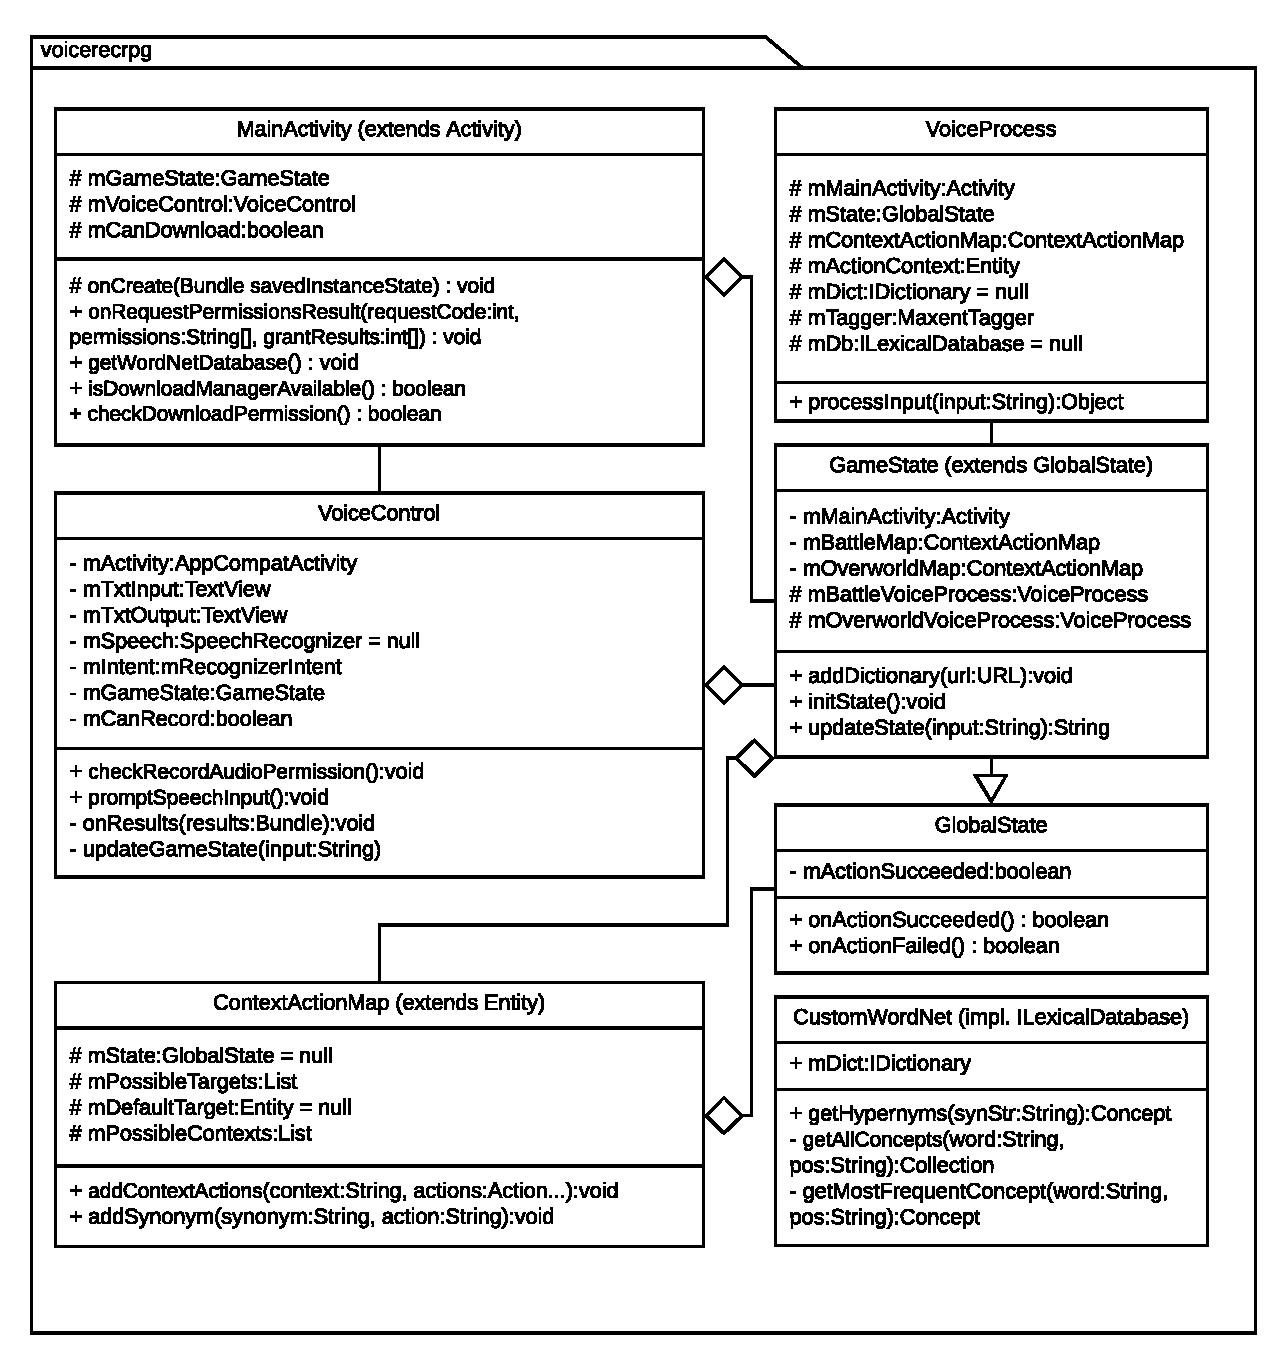
\includegraphics[width=\linewidth]{system-overview.pdf}
  \caption{A simplified UML class diagram outlining the design of the voice recognition system. Diagram created using the online LucidChart tool. See the Appendix \ref{appendix:system-uml} for the full class diagram for the entire voice recognition system in the Android application.}
  \label{fig:system-overview}
  \end{center}
\end{figure}
\end{center}

\subsubsection{\texttt{MainActivity} Class}

The \texttt{MainActivity} class is the skeleton class which contains all the systems. It acts as the interface between the I/O and the rest of the application. It contains instances of the \texttt{VoiceControl} class, which handles the I/O, and the \texttt{GameState}, which contains the game environment.
\\
\\
When the application starts up, an instance of \texttt{MainActivity} is created, and searches the public directory of the phone's external storage (not necessarily an external device like an SD card, but the directory which the OS has has defined the external storage to be). It searches for a WordNet database that is downloaded beforehand, and if it is not found, it will download/re-download the database again. It will also copy a model used for POS tagging to the external storage from the Android application package (APK) archive.

\subsubsection{\texttt{VoiceControl} Class}

The \texttt{VoiceControl} class is used to handle the input and output of the application, such as the microphone input and the text display. It contains an instance of the \texttt{SpeechRecognizer} class, which is provided by an Android SDK and uses Google's Speech-to-Text API, as well as two instances of the \texttt{TextView} class: one which is used to display the text output of the game, and the other to display the speech-to-text result at the top of the screen.
\\
\\
When the \texttt{SpeechRecognizer} instance performs a speech-to-text translation, the final result is forwarded to the \texttt{GameState} instance where it is processed by the voice recognition system using NLP, and used to update the state of the current game session in \texttt{GameState}.

\subsubsection{\texttt{VoiceProcess} Class}

The \texttt{VoiceProcess} class is responsible for processing the string input containing the player's utterance that is received from the \texttt{VoiceControl} class. It contains the majority of the NLP processing.

\subsubsection{\texttt{GlobalState} Class}

The \texttt{GlobalState} class is a generic abstract class that can be derived from in order to pass around environment objects between method calls easily. For example, if a method wishes to access an instance of an \texttt{Inventory} class (to access the game's items), then a reference to the inventory can be held in a class derived from \texttt{GlobalState} (e.g. \texttt{GameState}).

\subsubsection{\texttt{ContextActionMap} Class}

The \texttt{ContextActionMap} class contains the mapping of contexts to actions. It is an abstract class that is overloaded by the developer to add mappings of different ways of performing actions based on the given context (e.g. ``attack with a sword" versus ``attack with a hammer").

\subsubsection{\texttt{SemanticSimilarity} Class}

This class contains the semantic similarity engine used for calculating the semantic similarity of two words as a confidence value between 0.0 and 1.0, based on information in the WordNet database. It uses a singleton design pattern so the class does not have to be instantiated every time a calculation needs to be performed with a different method, nor does a reference to an instance need to be passed around everywhere it is used. It also allows us to use the same static instance across different Android Activity contexts (and therefore allow the engine's parameters to be changed in a \textit{Settings} screen).

\subsection{System Features}

In order to make the voice recognition system as flexible as possible and able to infer the meanings of a wide variety for utterances, several mechanisms have been added to the system. These mechanisms help to reduce the amount of work required by the developer, and some are present in order to compensate for the shortcomings of the system (see the Evaluation section).

\subsubsection{Synonym Mapping}

The developer can map synonyms to actions if the words are not considered semantically similar by the system. For instance, if the word, ``regenerate" has a low semantic similarity score when compared to the ``heal" action, then the developer can create a map of ``regenerate" $\rightarrow$ ``heal" so the system performs the correct mapping.

\subsubsection{Ignoring Incorrect Matches}

Semantic similarity matches can be ignored if they are incorrectly mapped by the system, as a juxtaposition to the above feature.

\subsubsection{Confirmation and Suggestions}

If the user gives a command that has a confidence value just below the threshold, then the phrase is considered ambiguous and, using the possible candidate matches, suggestions are given to the user to confirm their intent. 
\\
\\
For example, if the user's intent is to pick up a knife and they say, ``pick up the utensil", where the similarity score between ``utensil" and ``knife" is just below the threshold, the system will output, ``Did you mean, `pick up the knife? (yes/no)'", and waits for the user to respond. If they say no, then the system may suggest another alternative using the next ambiguous candidate (e.g, ``Did you mean, `pick up the plate?'", etc.).

\subsubsection{Multiple Commands}

The user has the ability to execute a chain of several commands one after the other using just one utterance. For example, if the user says, ``attack the enemy and then heal using a potion", this will execute two separate commands.

\subsubsection{Multiple Targets}

A user may want to execute a command that involves several targets. In this case, the intent is divided into several actions instead, with each action focused on one of the targets. For instance, if the user says, ``attack the troll and the goblin", this will be split into two actions: one to attack the troll, followed by an attack on the goblin.

\subsubsection{Sentence Mapping}
\label{section:sentence-mapping}

The core mechanism of the system is the slot-filling structure described previously. This covers most of the forms of possible imperative commands that a user may utter to the system to execute an intent. However, one disadvantage of this system is that it will not detect phrases that do not map to the slot-filling grammar given (e.g. \{\texttt{ACTION TARGET WITH CONTEXT}\}), despite being a valid phrase. Such utterances are usually phrased as a question, such as, ``What actions can I do?", or, ``What items are in my bag?", etc. (see Section \ref{section:eval-sfs} for a detailed evaluation of the chosen slot-filling grammar). The system should still be able to detect these types of commands but prevent the developer from hard-coding each possible variation of the intents.
\\
\\
The proposed solution is to perform sentence matching on these phrases. The developer specifies an intent followed by several example sentences that a user would say to execute the intent. For example, if the intent is to show the player the items they possess, example sentences would include: ``What is in my bag?", ``What items do I have?", ``What are the contents of my inventory?", and so on. When parsing a new utterance from the player (e.g. ``What items are in my bag?"), if the phrase fails the slot-filling stage, then the similarity of the sentence compared to the example sentences is calculated.
\\
\\
The calculation involves using a slightly altered cosine similarity method. Based on the formula for the cosine of an angle between two vectors, the cosine  similarity method measures uses the cosine of the angle as a measure of similarity, using a vector space model \cite{RefWorks:119} (the vector of a sentence is represented by its word frequencies). The similarity between two vectors, $a$ and $b$ is:

$$similarity = \cos \theta = \frac{a \cdot b}{\lvert a\rvert\lvert b\rvert}$$

Take two examples: ``the apples are in the tree" and ``the tree contains apples". The vectors for these sentences would be:

\begin{center}
a = \{the:2, apples:1, are:1, in:1, the:2, tree:1, contains:0\}
\\
b = \{the:1, apples:1, are:0, in:0, the:1, tree:1, contains:1\}
\end{center}

The cosine similarity of these sentences is therefore:

$$\frac{a \cdot b}{\lvert a\rvert\lvert b\rvert} = \frac{6}{2\sqrt{3} \cdot \sqrt{5}} = 0.77$$

The definition for cosine similarity has been altered to form a ``soft cosine measure" \cite{RefWorks:120}. This uses the semantic similarity between the two words (when the dot product is calculated) as a weighting: if a word only appears in one sentence and not he other, then the scores of its semantic similarity to the words in the other sentence are added to the numerator.
\\
\\
While the cosine similarity is not ideal for all situations (e.g. it ignores word order so may match two sentences which are not similar at all), it is easy to implement for the sentence matching mechanism, which is supplementary to the voice recognition system.

\subsection{Game Design Overview}

The voice recognition system will be applied to a text-based role-playing game that has several different modes of play, in order to demonstrate the flexibility of the system. The first mode is similar to the Zork-style text-adventure gameplay, mentioned previously. This involves the player interacting with objects in the environment to solve puzzles while collecting items, in order to progress. This mode is named the \textit{Overworld} mode.
\\
\\
The second mode of gameplay is similar to classic turn-based RPGs such as Pok\'emon or Final Fantasy, where the player battles an enemy, and the opposing sides alternate between taking turns to either attack, defend, heal, or perform some other action. This mode is called the \textit{Battle} mode.

\subsubsection{Game Flow}

The focus of the project is not on the game itself, but rather on the power and flexibility of the voice recognition system to add voice commands to the game. Therefore, only a simple game will be created with a few rooms, with different rooms focusing on different game modes (\textit{Overworld} or \textit{Battle}).
\\
\\
For the first room, the player is placed in a room where they are presented with a puzzle as part of the \textit{Overworld} mode. The room features the following description:

\begin{itemize}
\item ``You are in a room with a locked door in front of you.

\item ``There is a glass table in the middle of the room."

\item ``There is a knife on the table."

\item ``A painting of a tree hangs by a string on the left wall."
\end{itemize}

The player must obtain a key hidden behind the painting by cutting it down using the knife (or any other sharp item they may possess such as a sword), and then use the key to open the door.
\\
\\
During the \textit{Overworld} gameplay, the user is capable of performing the following actions:

\begin{center}
[look, show, grab, open, cut, break]
\end{center}

Example commands include, ``show my inventory", ``look around the room", ``grab the knife", ``cut the painting", and so on.
\\
\\
Each room in the game which features the \textit{Overworld} gameplay is represented by a finite state automaton. When the player performs certain actions (e.g. cutting the painting down), the state of the room will progress until the player has performed the correct  actions in the correct order and is able to progress to the next room. Figure \ref{fig:room1-fsa} show the state diagram for the first room.

\begin{center}
\begin{figure}[H]
\begin{center}
  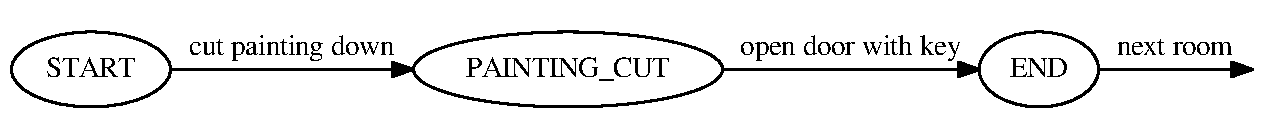
\includegraphics[width=\linewidth]{room1-fsa.pdf}
  \caption{The state diagram for one of the rooms in the game.}
  \label{fig:room1-fsa}
  \end{center}
\end{figure}
\end{center}

As part of the \textit{Battle} mode, the player will be presented with a battle against an enemy (e.g. a \textit{troll}). The following actions are available to the player:

\begin{center}
[attack, heal, show, look]
\end{center}

Examples include: ``attack the troll" ``heal with a potion", ``look around", and so on.

\subsection{Game Design UML Class Diagram}

Figure \ref{fig:game-overview} on page \pageref{fig:game-overview} shows a simplified UML class diagram for the game logic.
\\
\begin{figure}
\begin{center}
  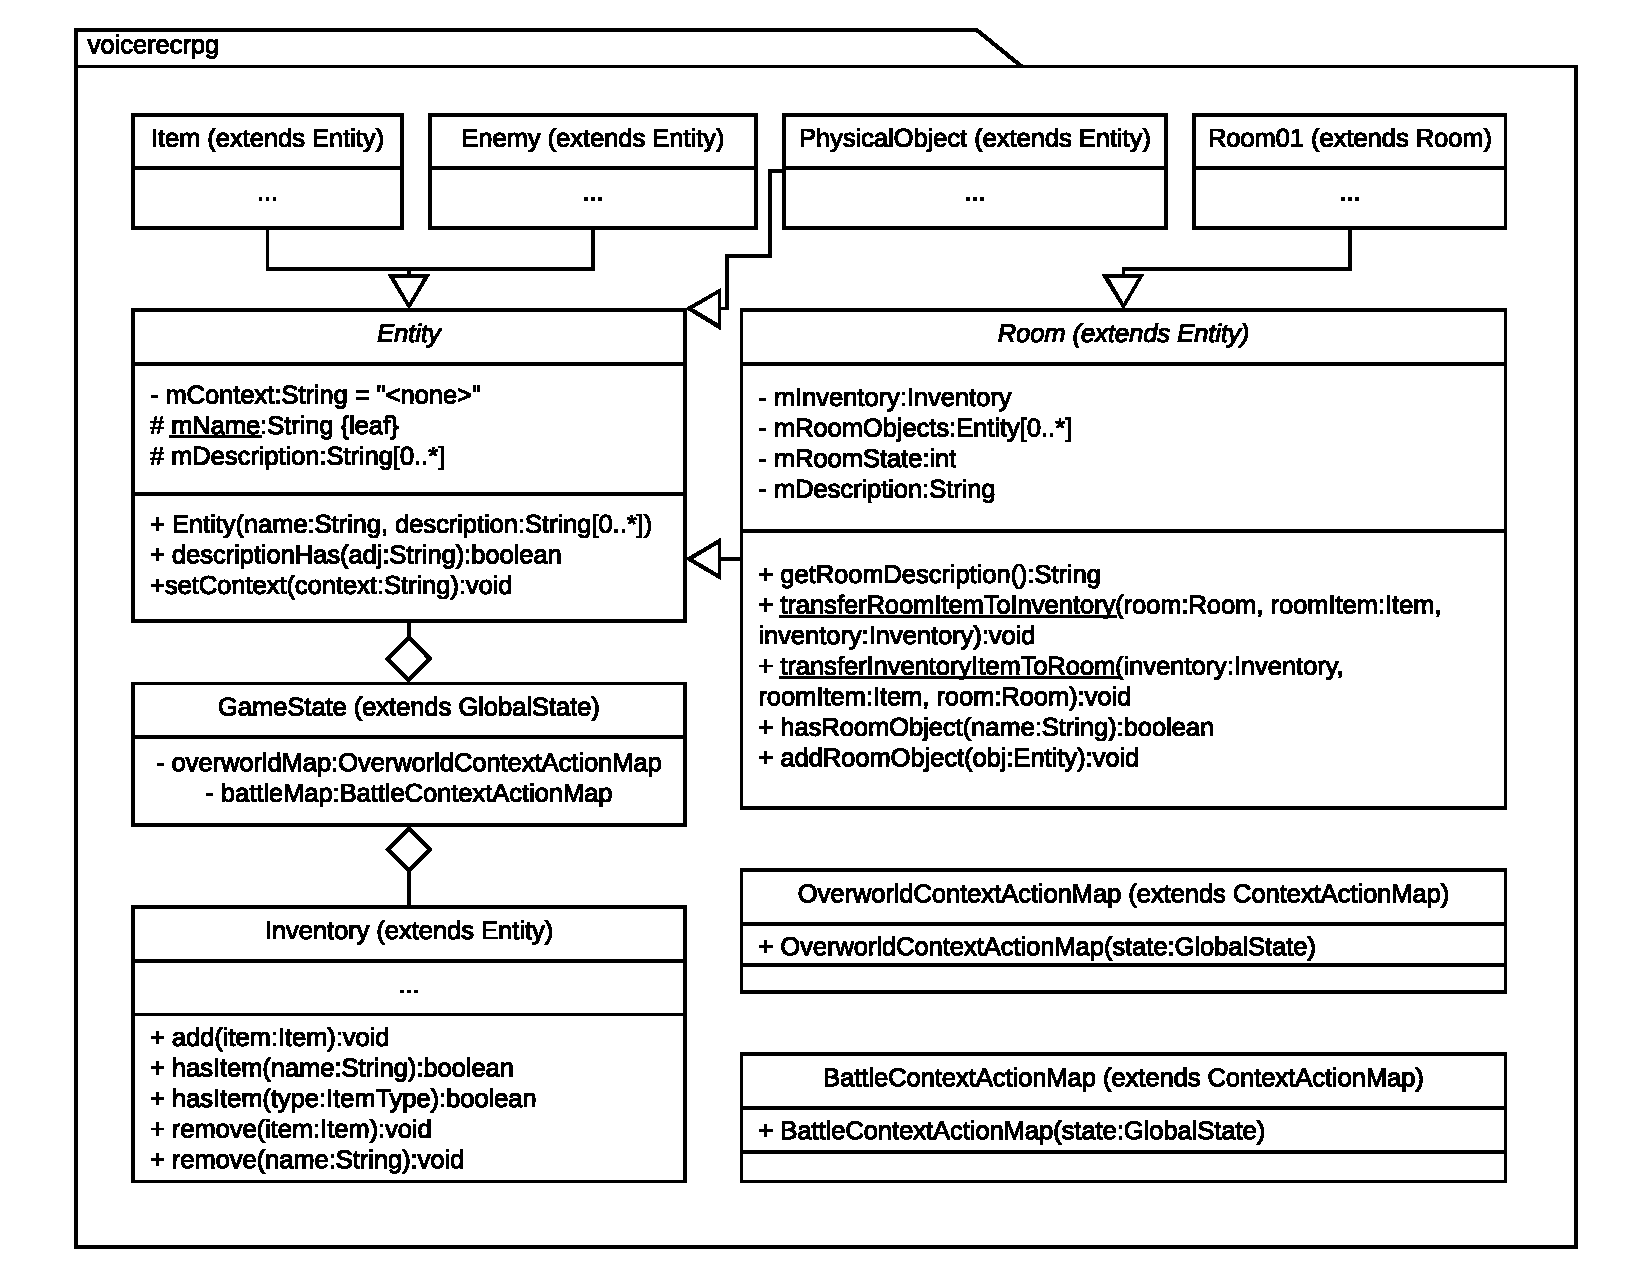
\includegraphics[width=\linewidth]{game-overview.pdf}
  \caption{A simplified UML class diagram outlining the design of the gameplay mechanics. Diagram created using the online LucidChart tool. See the Appendix \ref{appendix:game-uml} for the full UML class diagram.}
  \label{fig:game-overview}
  \end{center}
\end{figure}

The \texttt{GameState} class (shown previously in the system UML class diagram, to aid explanations) contains two different instances of classes that override the voice recognition system's \texttt{ContextActionMap} class (which contain the voice command mappings): one for the overworld gameplay and the other for the battling gameplay.
\\
\\
The \texttt{Entity} abstract class represents anything that can be considered a possible target or context for the slot-filling. Each entity is given a name and a context type (as a string) that is used to determine which context it maps to (e.g. ``weapon", ``key", etc.). See Table \ref{action-context-ex-table} above for examples of these contexts. Each entity also contains a description field which is an array of words that describe the entity (e.g. a knife would be described as ``sharp", ``pointy", etc.). These descriptions are optional but they aid the voice recognition system to help identify similar words (if the semantic similarity match fails).
\\
\\
Finally, \texttt{Room} is an abstract class for generating new rooms for the game, each with their own objects.

\newpage
\subsection{Room Generation}

Instead of forcing the developer to manually instantiate objects within each room, a mechanism will be written that will allow a developer to generate a new room from just a description of it, using natural language processing techniques.
\\
\\
A command-line program has been created which takes as input a text file containing a description of a room and generates a source file for a \texttt{Room} class, containing the objects from the description, and also handles object relations (e.g. whether a lamp is on the table or on the floor). This allows the developer to easily create new rooms for the game without having to manually add the objects to a room. See Section \ref{section:room-generation} for the implementation.

\newpage
\section{Implementation}

This section outlines the steps taken to implement the system and the game, mostly in chronological order where appropriate. For more details on the source code, please see the corresponding GitHub repository containing this project's work.\footnote{https://github.com/BaronKhan/VoiceRecognitionRPG}

\subsection{System Architecture}

Figure \ref{fig:component-diagram} shows a UML component diagram for the system architecture of the Android application. The front-end consists of three \texttt{Activity} classes. An \texttt{Activity} is the environment where the user interacts with the application.

\begin{figure}[H]
\begin{center}
  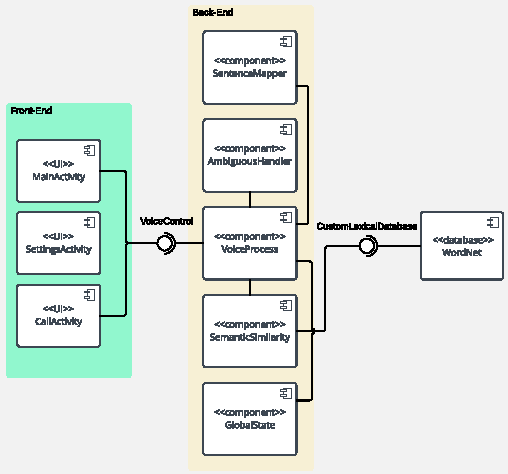
\includegraphics[width=\linewidth]{component-diagram.pdf}
  \caption{A UML component diagram showing the components of the application.}
  \label{fig:component-diagram}
  \end{center}
\end{figure}

The \texttt{MainActivity} is where the role-playing game interactions will take place, while the \texttt{CallActivity} contains a demo of the system applied to a video conferencing example (see Section \ref{section:calling-demo}). There is also a \texttt{SettingsActivity} for setting the different parameters of the application (see Section \ref{section:settings}).
\\
\\
The back-end accesses a WordNet database stored on the phone to perform similarity calculations through a \texttt{CustomLexicalDatabase} interface (see Section \ref{custom-lexical-database-impl} for more).

\subsection{Voice Recognition Interface}

The first step in the implementation involved creating an Android project with a skeleton I/O to take as input the microphone audio, converts the speech to text, sends it to the voice recognition system for processing (initially just an empty class that pipes the input to output), before finally displaying the text on the screen.
\\
\\
The interface is within the \texttt{MainActivity} class. When the activity is created, it also downloads a tar ball containing a WordNet database and unzips it on the device's local storage. While it is possible to package the database with the model, the code was originally written to download the database and, due to time constraints, could not be changed.
\\
\\
The \texttt{MainActivity} class contains a \texttt{VoiceControl} class that  handles the speech-to-text (STT) I/O, and implements a \texttt{RecognizerIntent}. The \texttt{VoiceControl} object contains an instance of the \texttt{SpeechRecognizer} class that has a \texttt{startListening()} method, which invokes an \texttt{onResults()} method when finished. This method has a \texttt{results} parameter of type \texttt{Bundle}, containing the string result of the speech recognition. The string is then processed by an instance of the \texttt{VoiceProcess} class (described below).

\subsection{Graphical User Interface}

Figure \ref{fig:snapshot-ui} shows a snapshot of the UI for the game logic with the following labels:

\begin{enumerate}
	\item A \texttt{TextView} element containing the player's input for the game as a string (i.e. it is the output of the speech-to-text API).
	\item A \texttt{TextView} containing the cumulative output of the game as each input is processed.
	\item Pressing this \texttt{Button} element activates the microphone and starts a voice intent.
	\item A timer used for debugging the time taken to process an intent by the system.
	\item This drop-down list contains various options (such as an option to open the settings menu).
\end{enumerate}

\begin{center}
\begin{figure}
\begin{center}
  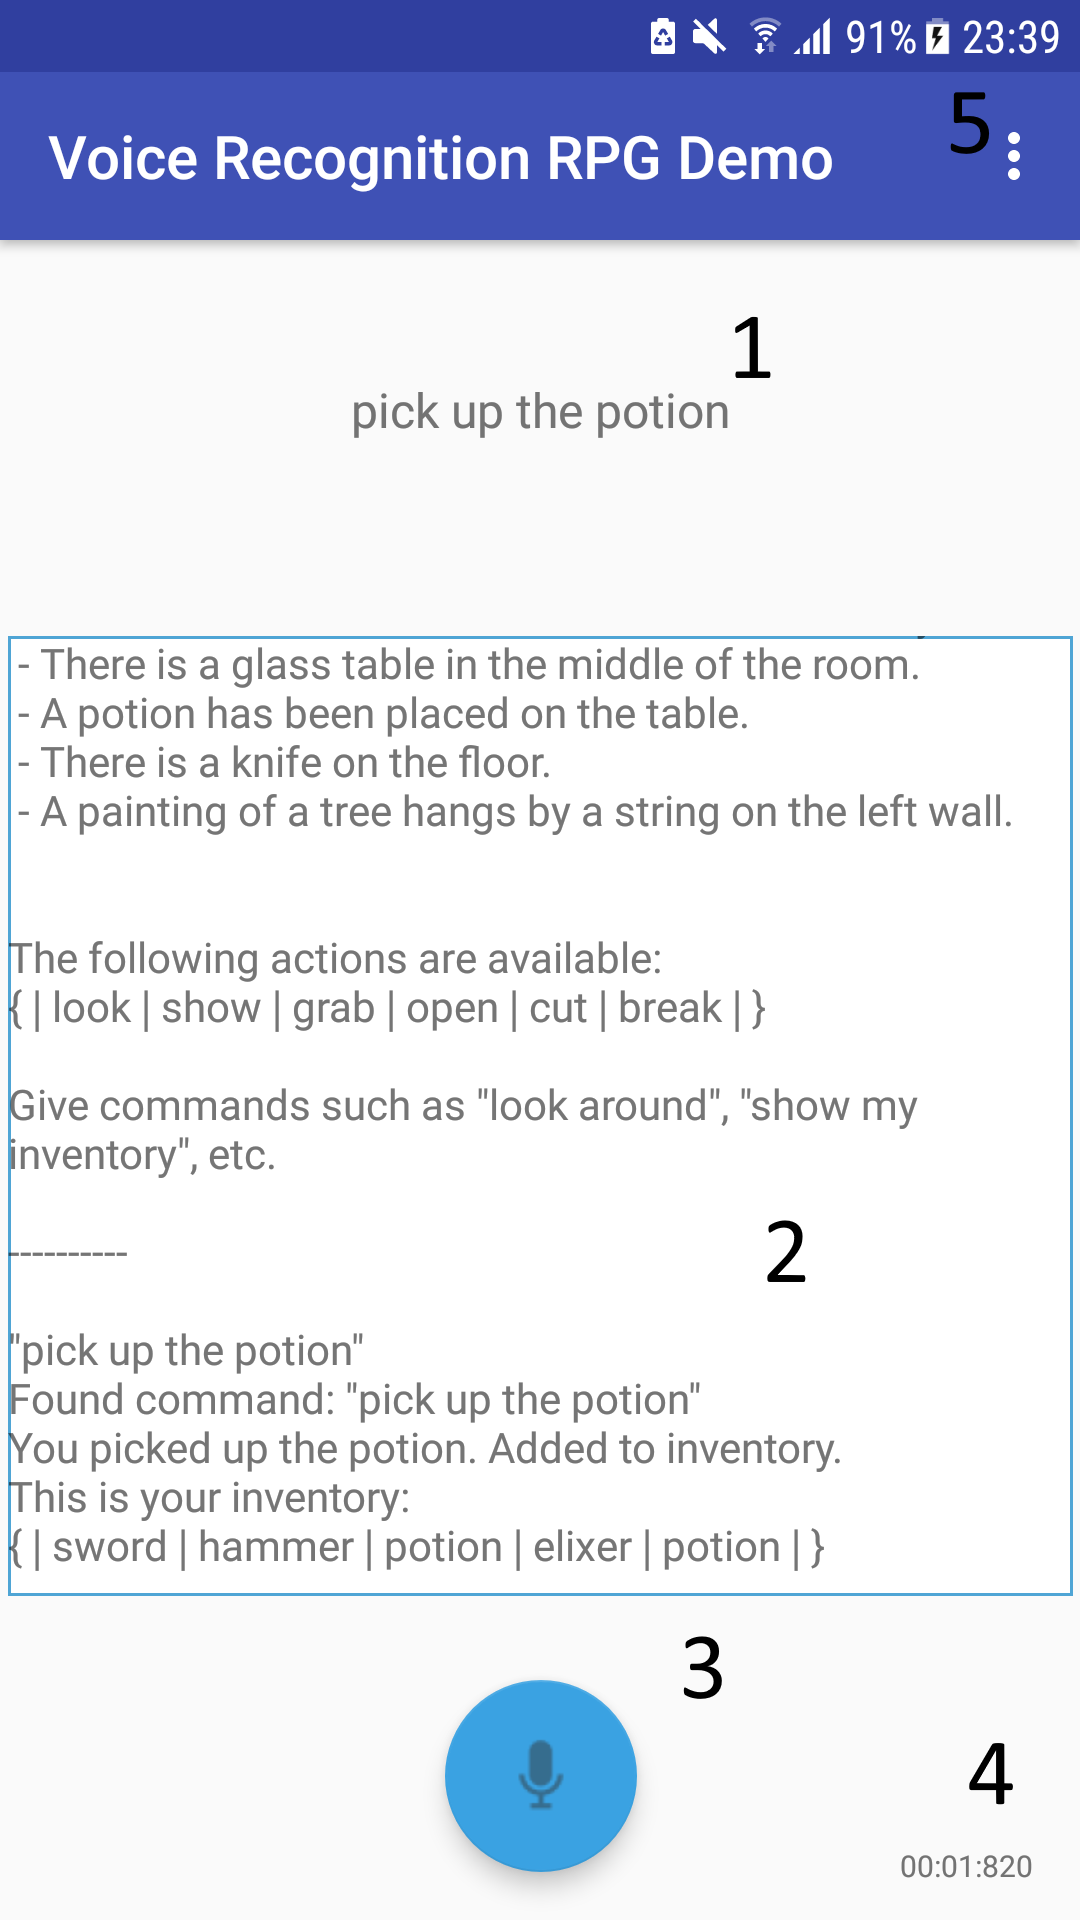
\includegraphics[scale=0.4]{Screenshot_20180519-233930.png}
  \caption{A snapshot of the user interface for the text-based role-playing game.}
  \label{fig:snapshot-ui}
  \end{center}
\end{figure}
\end{center}

All UI elements (such as \texttt{TextView}s, \texttt{Button}s, etc.) are accessed in the \texttt{MainActivity} class, and are separate from the voice recognition system.

\subsection{User Flow Diagram}

Figure \ref{fig:wireframe} shows a wireframe for the different screen transitions that occur as the user interacts with the application.

\begin{figure}[H]
\begin{center}
  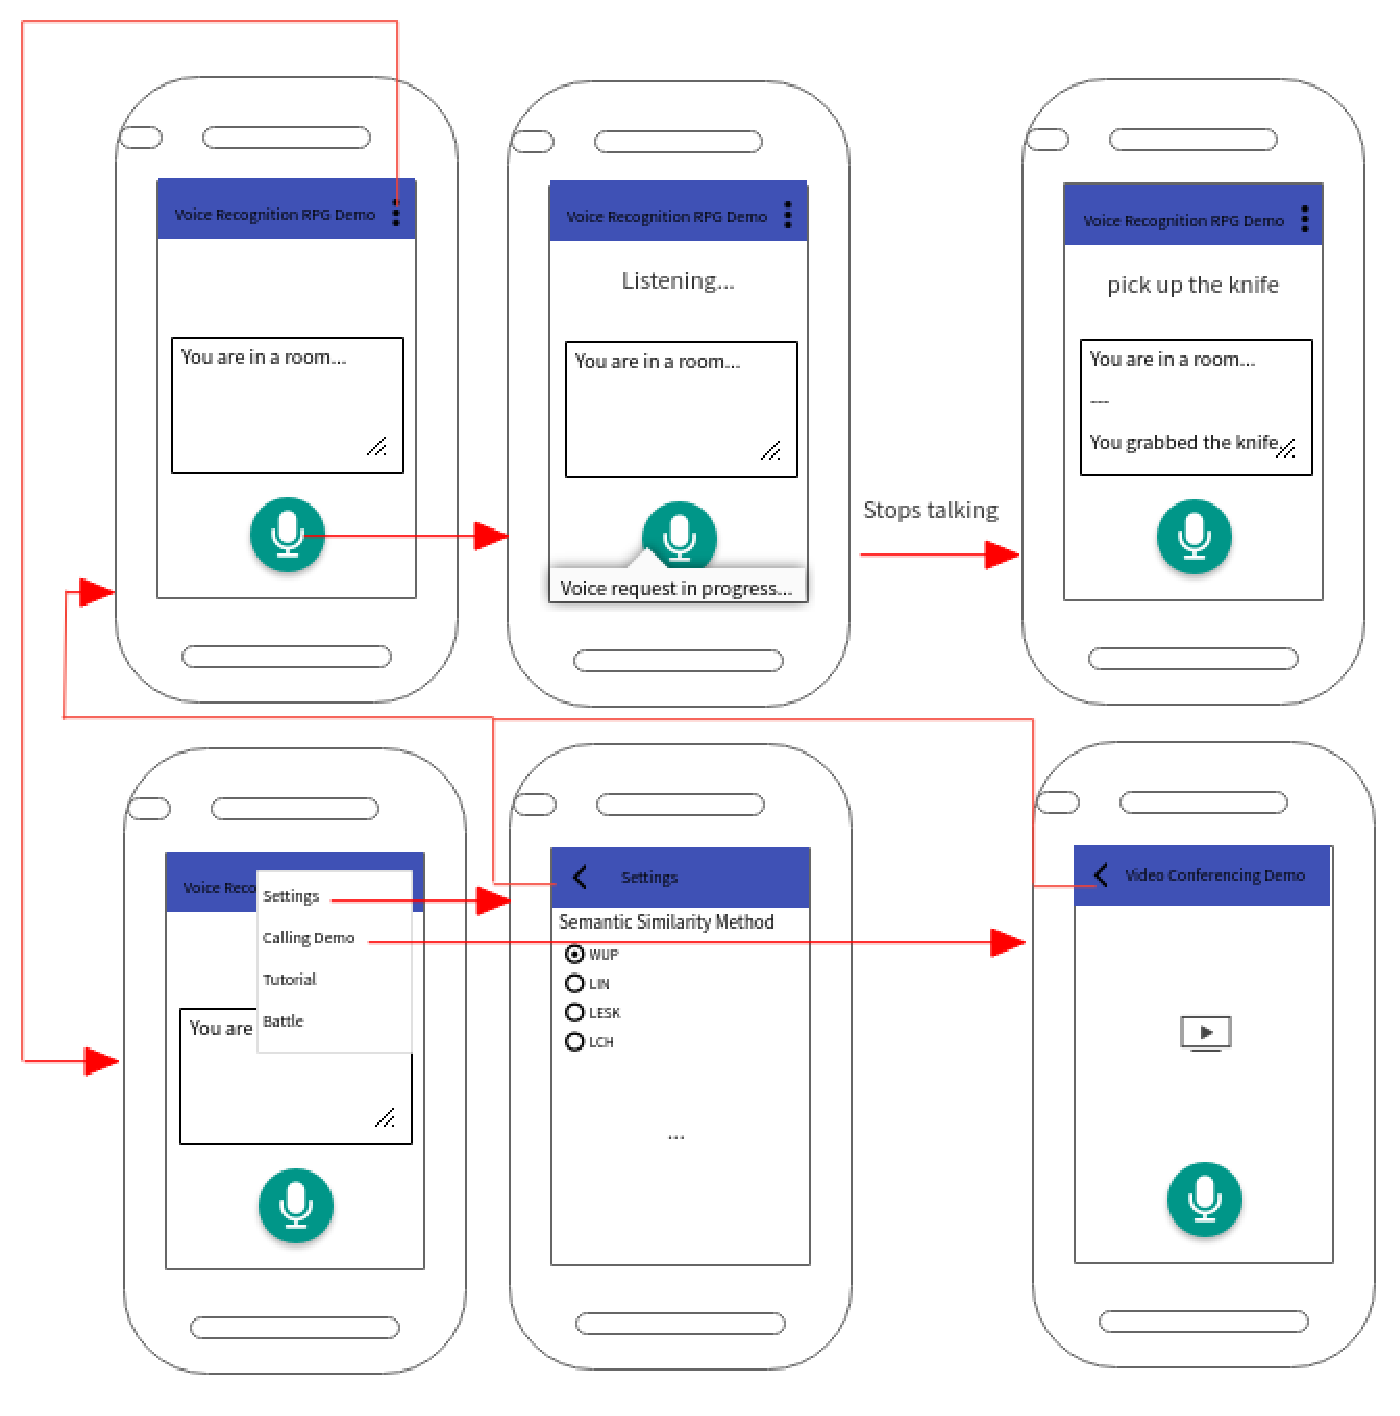
\includegraphics[width=\linewidth]{wireframe.pdf}
  \caption{A wireframe showing the majority of transitions between activities as the user interacts with the application. The tails of the red arrows indicate where the user touches the screen (unless otherwise stated). Diagram created using MockFlow.}
  \label{fig:wireframe}
  \end{center}
\end{figure}

\subsection{Voice Recognition System Implementation}

This section outlines the general process of understanding the user's intent and mapping it to an action in the application. It also describes each component in the voice recognition system in more detail.

\subsubsection{Data Flow Diagram}

Figure \ref{fig:data-flow} shows how data flows in the voice recognition system, starting from the user's audio input, and ending with the output sent to the UI. Note that not all data paths will be followed during a voice intent. The critical path is highlighted in red.

\begin{figure}[H]
\begin{center}
  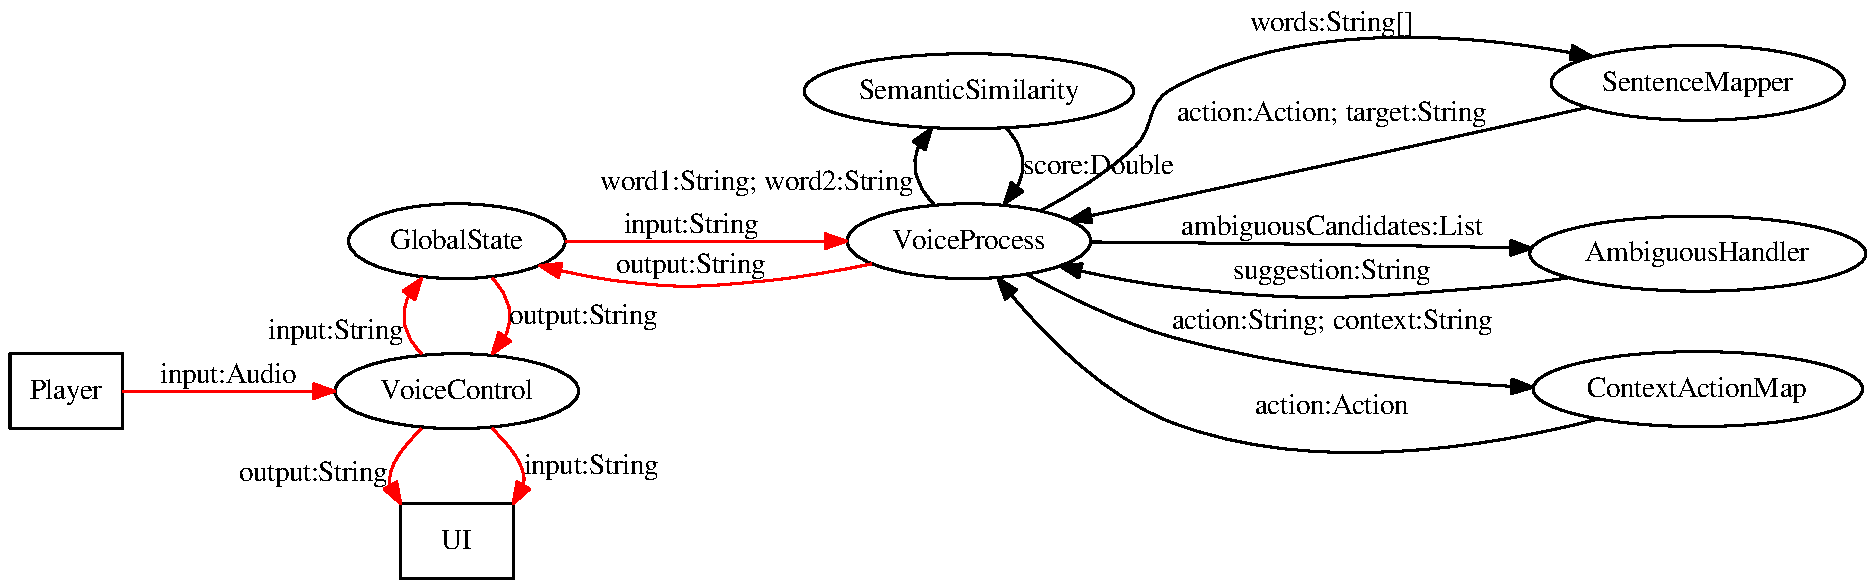
\includegraphics[width=\linewidth]{data-flow.pdf}
  \caption{A data flow diagram showing how the player's input (starting from 'Player') is processed by the different components until a response is sent to the 'UI'. The critical path is highlighted in red. Diagram generated automatically using Graphviz.}
  \label{fig:data-flow}
  \end{center}
\end{figure}

\subsubsection{\texttt{GlobalState}}

The \texttt{GlobalState} class is an abstract class that sends the string input to a \texttt{VoiceProcess} instance via the \texttt{updateState} method. Derived classes (e.g. \texttt{GameState} for a game, \texttt{KitchenState} for a cooking application, etc.) contain the application-specific logic and environment that can be accessed by the action methods.
\\
\\
In some scenarios, a follow-up action may only take place if the user's action was successful. For instance, in a generic two-player game, the second player may only be able to make their move once the first player has made a successful move. A more relevant example is in a turn-based role-playing game, where the player is fighting an enemy. The enemy can make their move once the player has made their move.
\\
\\
To support this scenario, there is a Boolean field called \texttt{mActionSucceeded}, which is set within the action methods that are executed to tell the system whether the action has succeeded, and the developer can choose what happens next.

\subsubsection{\texttt{VoiceProcess}}

\texttt{VoiceProcess.java} is the main class that performs all the processing on the text string input (of the user's utterance). The main method is the \texttt{processInput()} method that takes the string input and returns the response. Figure \ref{fig:process-input} shows a flow chart for this method.

\begin{figure}[H]
\begin{center}
  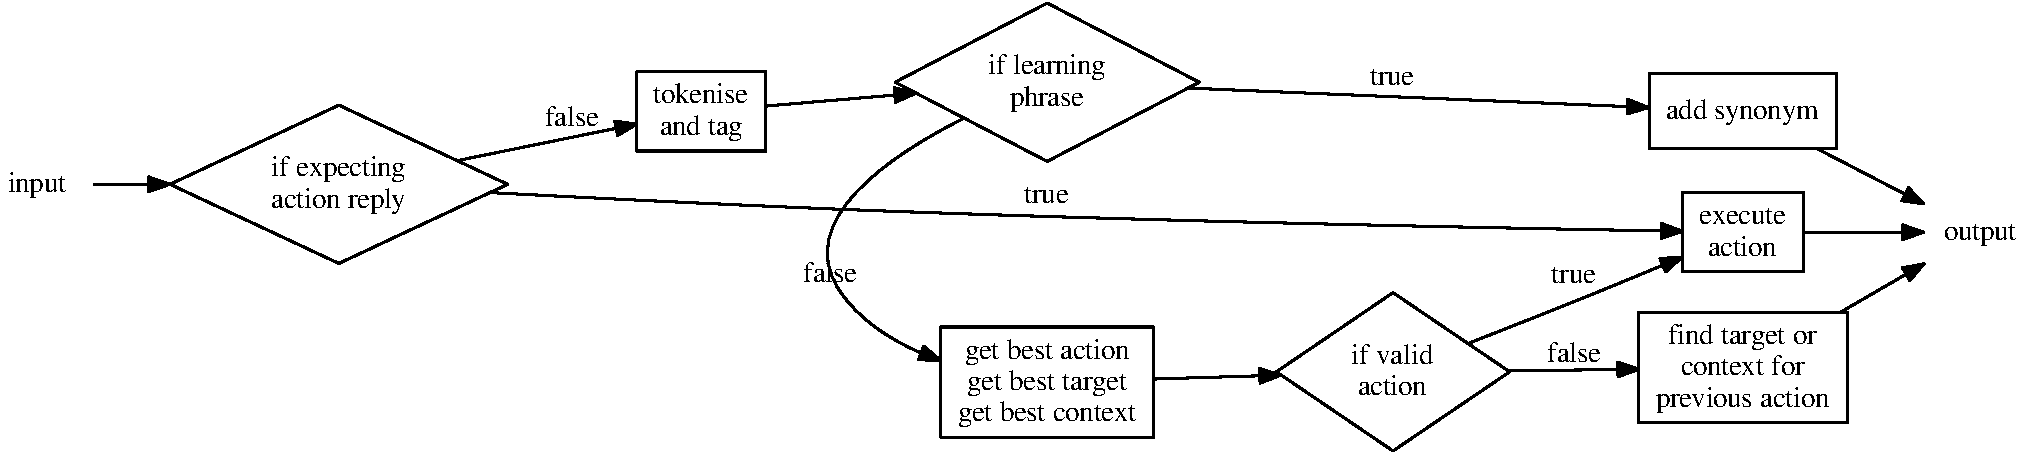
\includegraphics[width=\linewidth]{process-input.pdf}
  \caption{A flow chart outlining the \texttt{processInput()} method in the \texttt{VoiceProcess} class. Note that any minor steps are not shown here.}
  \label{fig:process-input}
  \end{center}
\end{figure}

Listing \ref{lst:voice-process-pseudo} shows the pseudocode for the method, with most of the minor details removed. For the full Java method, refer to the source code in the project's repository.

\begin{lstlisting}[caption=Pseudocode for processInput(), label={lst:voice-process-pseudo}]
def processInput(input):
    checkIfWordNetIsLoaded()
    
    if expectingReply:
        return processPendingIntent(input)
    
    //Check for action replies
    if currentAction.wantsReply():
        return currentAction.processReply(input)
    
    words, tags = tokeniseAndTag(input)
    
    //Check for learning phrase ("___ means ___")
    if words.size() == 3 and words.contains("means"):
        addSynonym(words[0], words[2])
    
    //Parse the input
    actionIndex, chosenAction = getBestAction(words, tag)
    
    if isValidAction(actionStr):
        chosenTarget = getBestTarget(words, tags)
        chosenContext = getBestContext(words, tags)
        
        if not isValidContext(bestContext):
                or contextActionMap.get(chosenContext).get(chosenAction) == null:
            chosenContext = "default"
            
        action = contextActionMap.get(chosenContext).get(chosenAction)
        if action == null:
            return "Intent not understood."
        else:
            if isAmbiguous():
                return suggestion()	//Did you mean...?
            else:
                 return action.execute(state, chosenTarget)
    else:
    	//Check for another target for previous action
        if foundAnotherTarget(words, tags):
            currentTarget = getBestTarget(words, tags)
            return previousAction.execute(state, currentTarget)
        else if foundAnotherContext(words, tags):
            currentContext = getBestContext(words, tags)
            return previousAction.execute(state, currentContext)
        else:
            performSentenceMatching(input)
\end{lstlisting}

When tokenising and tagging the input, a list of \texttt{words} and a list of \texttt{tags} are created. The index of a word in \texttt{words} corresponds to the index of its tag in \texttt{tags}.
\\
\\
For the \texttt{getBestAction()}, \texttt{getBestTarget()} and  \texttt{getBestContext()} methods, the words in the input are checked sequentially to determine the best match. For instance, in the \texttt{getBestAction()} method, the candidate actions are first chosen from the input. For each candidate action, a score out of 1.0 is calculated against each possible action defined in the \texttt{ContextActionMap}: if the words match character-by-character or the candidate is a synonym for one of the actions, then the score is set to 1.0. Otherwise, the score is set to the semantic similarity score of the two words. The \texttt{getBestTarget()} and \texttt{getBestContext()} methods work similarly.
\\
\\
The candidates are chosen using POS tagging, to filter out words with no meaning such as ``the", ``it", etc. Words in the input are candidate actions if they are tagged as either a verb, adverb, or noun (occasionally, the POS tagger incorrectly tags some imperative verbs as nouns).

\subsubsection{\texttt{AmbiguousHandler}}

Candidate actions, targets and contexts may be marked as ambiguous/uncertain if their confidence score is just below a threshold value. If the best action/target/candidate has a confidence value lower than this threshold, then all the ambiguous candidates are queried to the user using the \texttt{AmbiguousHandler} class. This class will generate a suggestion and display it to the user, starting with the ambiguous candidate which gave the highest confidence. If the user disagrees with the suggestion (i.e, they say ``no" or something similar), then the next suggestion is given, until no more suggestions are available.
\\
\\
Figure \ref{fig:snapshot-suggestion} shows an example of a suggestion displayed to the user after an ambiguous intent. See the \texttt{AmbiguousHandler.java} file in the project's repository for the full code.

\begin{figure}
\begin{center}
  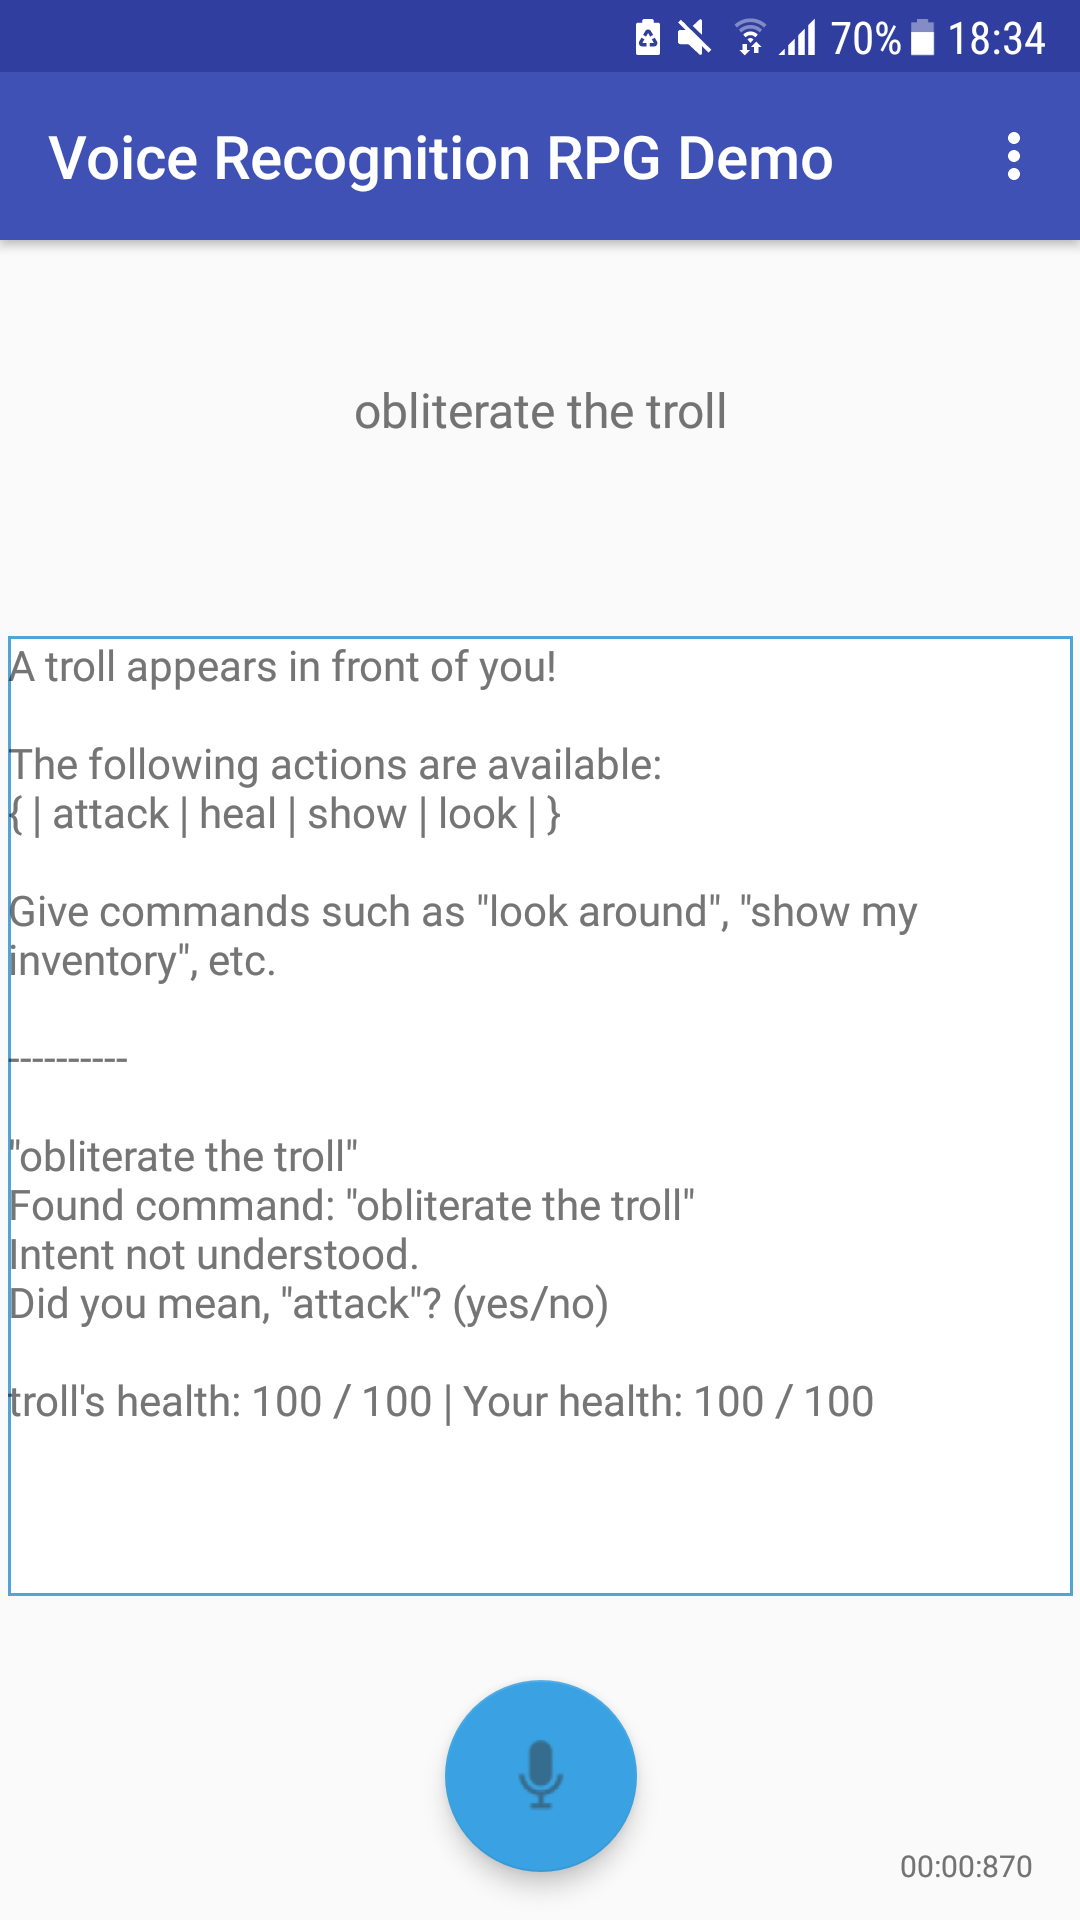
\includegraphics[scale=0.25]{Screenshot_20180522-183411.png}
  \caption{A snapshot of the ambiguous user intent, ``obliterate the troll". Here, the word, `obliterate' is most semantically similarity to the `attack' action, but not enough to pass the threshold, so it is queried to the user.}
  \label{fig:snapshot-suggestion}
  \end{center}
\end{figure}

\subsubsection{\texttt{SemanticSimilarity}}
\label{section:semantic-impl}

The semantic similarity engine is implemented as a singleton design pattern with a private constructor and a private instance of itself within the class. The main method of the class is the \texttt{calculateScore()} method which returns the semantic similarity score for two words.
\\
\\
The engine uses up to two semantic similarity methods, and if two are chosen, then the score returned is the average score from both methods. As well as the Wu and Palmer (WUP), Lin and Lesk methods mentioned previously, below is a list of methods that can also be chosen: 

\begin{itemize}
\item Fast Lesk (FASTLESK) - a faster implementation of the Lesk method, that removes string formatting of definitions and ignores meronym and holonym definitions of the words.

\item Path-based (PATH) - a simpler version of the WUP method which uses the reciprocal of the shortest path between the words in the WordNet database as the similarity score \cite{RefWorks:46}.

\item Leacock and Chodorow (LCH) - another path-based measure which uses the negative log of the shortest distance between the two words \cite{RefWorks:46}.

\item Resnik (RES) - similar to the LIN method, but does not normalise the information content of the words' least common subsumer \cite{RefWorks:46}.

\item Cosine (COS) - similar to the Lesk method, but uses the cosine similarity of their definitions (as opposed to just overlaps in the definitions).
\end{itemize}

Most of the above similarity method implementations are provided by the WS4J library, except the FASTLESK and COS methods, which are unique to this project and are implemented manually in the code (though the FASTLESK method is altered from WS4J's LESK method which was decompiled using Android Studio's built-in Fernflower decompiler \cite{RefWorks:124}). By default, only the WUP method is used by the system, though other methods can be chosen in the application's settings.

\subsubsection{\texttt{CustomLexicalDatabase}}
\label{custom-lexical-database-impl}

Despite the WS4J library providing implementations of the algorithms for most of the semantic similarity methods used in this project, they require an interface to be implemented in order to access a WordNet database, called \texttt{ILexicalDatabase}.
\\
\\
The WS4J library is packaged with its own implementation of \texttt{ILexicalDatabase} interface, called \texttt{NictWordNet} (which accesses a Japanese WordNet database similiar to the Princeton WordNet \cite{RefWorks:122}). Unfortunately, due to its use of SQLite methods to access the database, the implementation is not compatible with the Android SDK, and could not be used. Moreover, even if the SQLite methods worked, it would still require a connection to the internet in order to access the WordNet database, which is undesirable for this project, as one of the goals is to create a system that works entirely offline.
\\
\\
Therefore, a new implementation of the \texttt{ILexicalDatabase} interface was created that works with the Android SDK, called \texttt{CustomLexicalDatabase.java}. It interfaces with a local Princeton WordNet database using the MIT JWI API mentioned previously. All methods were implemented using the JWI API except the \texttt{findSynsetBySynset()} and \texttt{conceptToString()} methods (these methods are not required for the above similarity methods).
\\
\\
Since this implementation using the JWI library may be useful for others in the future, a GitHub gist has been published online (renamed to \texttt{JwiLexicalDatabase.java}) that other developers may freely use \footnote{https://gist.github.com/BaronKhan/5679157d1a8572debc8c75af1c875c16}.

\subsubsection{\texttt{ContextActionMap}}
\label{section:context-action-map}

The \texttt{ContextActionMap} class contains the table of mappings of contexts to intents. The developer uses this abstract class to create a derived class that defines the mapping in a `table' format (with contexts on the left and actions along the top) in the constructor. The table itself is implemented as a 'map of maps'. The \texttt{setActionsList()} method specifies the possible actions, while the \texttt{addContextActions()} method describes which Java method should be invoked for each action based on the context. The entries in the `table' are either \texttt{null} or classes that inherit from the \texttt{Action} class (see Section \ref{section:action}).
\\
\\
There is also an \texttt{addDefaultContextActions()} method, which defines the actions to be called if no context is given in the input. A \texttt{null} entry means that the action is invalid for the given context (e.g. you cannot attack with a potion). In this case, the default context action is called instead, and if the default action is \texttt{null}, then nothing happens.
\\
\\
Listing \ref{lst:game-context-action-map} shows an example of a derived class to create a table. Note that this example was only used for testing and evaluation of the system, and is not one of the tables used in the RPG demo.

\begin{lstlisting}[language=Java, caption=Example of a ContextActionMap, label={lst:game-context-action-map}]
public class GameContextActionMap extends ContextActionMap {
    public GameContextActionMap(GlobalState state) {
        super(state);
        setActionList(              "attack",        "heal",           "move");
        addDefaultContextActions(   new Attack(),    new Heal(),       new Move());
        addContextActions("weapon", new AtkWeapon(), null,             null);
        addContextActions("potion", null,            new HealPotion(), null);
    }
}
\end{lstlisting}

In order to make it easier for the developer to create this `table', a Python script was written called \texttt{generateTable.py} which takes as input a CSV file of a table, and generates a Java source file similar to Listing \ref{lst:game-context-action-map}. Table \ref{table:game-map-csv} shows the CSV table (where cells are separated by commas) that will generate the Java source file in Listing \ref{lst:game-context-action-map} using the command, 

\begin{center}
\texttt{python generateTable.py game-map.csv GameContextActionMap}
\end{center}

See the source code in the project's repository for the full Python script.

\begin{table}[H]
\centering
\caption{game-map.csv}
\label{table:game-map-csv}
\begin{tabular}{l|l|l|l|}
\cline{1-4}
\multicolumn{1}{|l|}{\textbf{}} & \textit{attack}    & \textit{heal}  & \textit{move}    \\ \hline
\multicolumn{1}{|l|}{\textit{default}} & Attack    & Heal  & Move    \\ \hline
\multicolumn{1}{|l|}{\textit{weapon}}  & AtkWeapon &            &  \\ \hline
\multicolumn{1}{|l|}{\textit{potion}}  &                & HealPotion &              \\ \hline
\end{tabular}
\end{table}

In the \texttt{ContextActionMap} class, there are two member fields that the developer must build in their application: the \texttt{mPossibleTargets} and \texttt{mPossibleContexts} lists. These are lists of objects that extend the abstract \texttt{Entity} class. Only entities in these lists are used in the target/context matching (when finding the best match).

\subsubsection{\texttt{Entity}}
\label{section:entity}

\texttt{Entity} is an abstract class in the system which represents anything that could be a possible target or context. Each derived class of \texttt{Entity} must set the following fields: \texttt{mContext}, which is the context type of the entity (i.e. the left-hand side value in a ContextActionMap described in Section \ref{section:context-action-map}); \texttt{mName}, which is the name of the entity (e.g, ``sword", ``potion", etc.), and, optionally, \texttt{mDescription}, which is a string array of adjectives that are used to describe the entity. \texttt{mDescription} is optional, but it assists the \texttt{processIntent} method in the \texttt{VoiceProcess} class in identifying the best matches for targets and contexts.
\\
\\
Once a match for a context is found, its \texttt{mContext} string value is used to index the \texttt{ContextActionMap} table, along with the chosen action.

\subsubsection{\texttt{Action}}
\label{section:action}

The \texttt{Action} class is an abstract class that is used to wrap the methods that should be executed in the \texttt{ContextActionMap}. The \texttt{execute()} method is overridden by the derived class and executed when the action is chosen in the \texttt{VoiceProcess} class. The method takes as input the GlobalState object (so the method can update its state if needed) and the current target (if it exists).
\\
\\
Some methods may wish to ask the user for confirmation before executing (e.g. ``Are you sure you want to do this?"). In this case, the \texttt{execute()} method would set the \texttt{mWantsReply} member field to \texttt{true}. On the next user intent, the input is processed by the \texttt{processReply()} method (i.e. whether the user said ``yes"/``no", etc.).

\subsubsection{\texttt{MultipleCommandProcess}}

Optionally, the developer can enable the ability to execute multiple commands with a single utterance. For instance, the player can say, ``attack the troll with a sword and then heal with a potion"; this would execute the attacking and healing as separate intents. The developer can wrap their \texttt{VoiceProcess} class inside a \texttt{MultipleCommandProcess} class.
\\
\\
The \texttt{MultipleCommandProcess} class has a \texttt{splitInput()} method which splits the user's input using the words, ``and" and ``then" as delimiters. It stores each result in a queue, and then processes each intent using the \texttt{executeCommand()} method, which takes the queue as input. If an intent is interrupted and more user input is required before continuing (e.g. if one of the intents is ambiguous, or an action requires a reply), then the remaining intents are stored in a second queue, and are processed once the current intent is resolved. See the Appendix \ref{appendix:multiple-commands-ex} for an example of the aforementioned scenario. Also see the \texttt{executeCommand()} method in \texttt{MultipleCommandProcess.java}.

\subsubsection{\texttt{SentenceMapper}}

The \texttt{SentenceMapper} is used to match sentences provided by the developer which do not fit the default slot-filling grammars (e.g. question-based intents). Each instance of \texttt{ContextActionMap} holds a reference to an instance of a \texttt{SentenceMapper}. Invoking the \texttt{addSentenceMatch()} method in the \texttt{ContextActionMap} class will add a map of several example utterances to an action and target.
\\
\\
The sentence mapper is run at the very end of the \texttt{processInput()} method of the \texttt{VoiceControl} class, if the slot-filling matching failed. A disadvantage to this is that the example sentences should not be able to be matched to the slot-filling grammar.
\\
\\
The \texttt{checkSentenceMatch()} method of the \texttt{SentenceMapper} class goes through each group of sentences, and calculates the average similarity of each group of sentences to the user's utterance, and matches with the highest value (if it is greater than a threshold value).
\\
\\
The similarity of each sentence with the utterance is based on the cosine similarity of the sentences (refer to Section \ref{section:sentence-mapping}). First, a vector of each sentence is created (which is just a map of the words to the word count) before the formula for cosine similarity is applied. Listing \ref{lst:cos-score} shows the code for this method.

\begin{lstlisting}[language=Java, caption=SentenceMapper.calculateCosScore(), label=lst:cos-score]
private double calculateCosScore(List<String> words1, String sentence) {
    Map<String, Integer> vector1 = getVector(words1);
    Map<String, Integer> vector2 = getVector(sentence);

    //Get common keys
    double numerator = 0.0;
    for (Map.Entry<String, Integer> entry1 : vector1.entrySet()) {
        for (Map.Entry<String, Integer> entry2 : vector2.entrySet()) {
            if (entry1.getKey().equals(entry2.getKey())) {
                numerator += entry1.getValue() * entry2.getValue();
            } else {
                numerator += 0.25*min(SemanticSimilarity.getInstance().calculateScore(
                        entry1.getKey(), entry2.getKey()) *
                        (entry1.getValue() * entry2.getValue()), 1.0);
            }
        }
    }

    double sum1 = 0.0;
    for (Map.Entry<String, Integer> entry1 : vector1.entrySet()) {
        sum1 += pow(entry1.getValue(), 2);
    }

    double sum2 = 0.0;
    for (Map.Entry<String, Integer> entry1 : vector2.entrySet()) {
        sum2 += pow(entry1.getValue(), 2);
    }

    double denominator = sqrt(sum1) + sqrt(sum2);

    if (denominator <= 0.0) { return 0.0; }
    else { return numerator / denominator; }
}
\end{lstlisting}

A disadvantage to running the sentence-matching at the very end is that the input may accidentally match to the slot-filling grammar. For example, if the user says, ``what can i cut?", and ``cut" is an action in the game, then it may map to the cut action, and not reach the \texttt{SentenceMapper}.

\subsubsection{Synonym Mapping Implementation}

Synonyms are used to aid the \texttt{VoiceProcess} system to match more words that the semantic similarity engine does not match automatically (due to a low similarity score). For example, the word, `obliterate' has a low similarity score to `attack' (below the threshold) even though they are very similar. Therefore, either the player or developer can add this mapping such that `obliterate' maps to `attack'.
\\
\\
The following are the possible ways of adding a synonym mapping:

\begin{itemize}
\item Add the synonym in the code (e.g. \texttt{addSynonym("obliterate", "attack")}).

\item The synonym is added when the same ambiguous intent is spoken twice (e.g. when the system asks the user, ``Did you mean, `attack'?" twice, and the user replies with ``yes" twice).

\item The player defines the mapping as an intent (i.e. they say, ``obliterate means attack"). See line 17 of the pseudocode in Listing \ref{lst:voice-process-pseudo} on page \pageref{lst:voice-process-pseudo}.
\end{itemize}

In some cases, a word could become a synonym for multiple words. Take the following scenario:

\begin{itemize}
\item The player is in a room with just a knife. The player utters, ``pick up the utensil", and creates a mapping from ``utensil" to ``knife".

\item The player progresses to a room with just a fork. They create a mapping from ``utensil" to ``fork".

\item The player is now in a room with both a knife and a fork, and says, ``pick up the utensil".
\end{itemize}

In this scenario, the system will use the \texttt{AmbiguousHandler} to ask the user whether they meant the knife or the fork. See the Appendix \ref{appendix:utensil} for the room that demonstrates this scenario (as well as room with multiple utensils, in which case, all suggestions are displayed at the same time).

\subsection{Role-Playing Game Implementation}

Simple rooms were created to demonstrate the system working with a typical text-based role-playing game. The first room of the game focuses on the \textit{Overworld} gameplay, and has a door which leads to a battle with an enemy (transitioning to the \textit{Battle} mode).

\subsubsection{GameState.java}

\texttt{GameState} is derived from \texttt{GlobalState} and acts as the `environment' for the game; it contains all the game's objects and handles the current state.
\\
\\
Since there are two distinct modes of gameplay (the \textit{Battle} gameplay and the \textit{Overworld} gameplay), there is a \texttt{ContextActionMap} for each one in the \texttt{GameState} class. It also keeps track of various data such as the current game mode; the current room/enemy; and the player's health.
\\
\\
The \texttt{GameState} class also has an instance of the \texttt{Inventory} class. This is a list of items currently in the player's possession. The player can transfer items from their inventory to the room and vice versa.

\subsubsection{Battle Mode}

In the \textit{Battle} mode, the player is able to attack the enemy with a wepon in their inventory. If no weapon is specified in the intent (as the context), then a random weapon is selected from the inventory, and if no weapon is available, the player attacks the enemy with their bare hands. The player can also heal using any healing items they have (e.g. potions, elixers, etc.), as well as look at their inventory or the available actions. Figure \ref{fig:battle-context-action-map} shows the `table' of action mappings for the \textit{Battle} mode. See the full \texttt{BattleContextActionMap} class in the project's source code (including the helper features such as synonym maps and sentence matches).

\begin{center}
\begin{figure}[H]
\begin{center}
  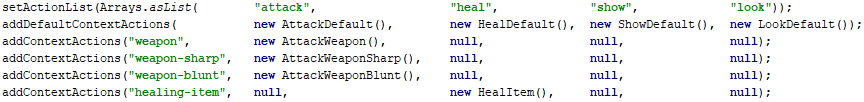
\includegraphics[width=\linewidth]{battle-context-action-map.png}
  \caption{A snapshot of the context-action `table' in \texttt{BattleContextActionMap.java}.}
  \label{fig:battle-context-action-map}
  \end{center}
\end{figure}
\end{center}

Weapons can be classified as either ``sharp" or ``blunt" based on whether they are instantiated with a description containing one of those words - each type of weapon as has different multiplier for the damage caused to the enemy.
\\
\\
Enemies are entities with their own health that the player fights. The enemy in the demo is a troll that can attack the enemy once the player has performed a successful action.
\\
\\
See the Appendix \ref{appendix:battle-mode-screenshots} for screenshots of examples of actions performed during the \textit{Battle} mode. Also see the Appendix \ref{appendix:battle-examples} for examples of commands that can be used during this mode.

\subsubsection{Overworld Mode}

In the \textit{Overworld} mode, the player interacts with objects in order to solve puzzles and progress to the next room. Figure \ref{fig:overworld-context-action-map} shows the `table' of action mappings for the \textit{Overworld} mode. Refer to the project repository for the full \texttt{OverworldContextActionMap} class.

\begin{center}
\begin{figure}[H]
\begin{center}
  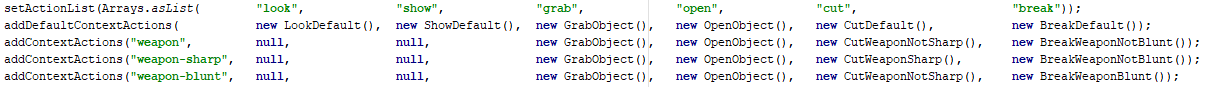
\includegraphics[width=\linewidth]{overworld-context-action-map.png}
  \caption{A snapshot of the context-action `table' in \texttt{OverworldContextActionMap.java}.}
  \label{fig:overworld-context-action-map}
  \end{center}
\end{figure}
\end{center}

Objects in the room can inherit from the \texttt{PhysicalObject} class, and can have properties such as whether they are breakable, whether they can be cut or scratched, etc.
\\
\\
See the Appendix \ref{appendix:overworld-examples} for examples of commands that can be used during the \textit{Overworld} mode. Also see the Appendix \ref{appendix:overworld-mode-screenshots} for screenshots of the first room in the game, and the actions required to solve the puzzle in the room.

\subsection{Object Properties with WordNet}

Using the semantic similarity engine, a user can select an item to use/interact with based on its chracteristics. For example, if the user possesses a sword in their inventory and says, ``attack with something sharp", the sword will be selected because the adjective, ``sharp" has a high similarity score to ``sword". Similarly, the word, ``heavy" has a high similarity to score to ``hammer", so if the player says, ``hit with something heavy", the hammer will be used.
\\
\\
In order to aid this system, entities can also be given a list of words (\texttt{mDescriptionList}) which describe the object.  This aids the voice recogntion system in identifying objects with characteristics that the user has specified.
\\
\\
Note that these properties associated to objects are separate from the properties in \texttt{PhysicalObject}, which are related to interactions specific in the \textit{Overworld} gameplay (e.g. whether an object is breakable), although these physical properties can be automatically assigned using the \texttt{autoAssignProperties()} method, which uses the semantic similarity engine to compare the name of the object to words associated with the property. The methods that do this are shown below. Note that "scratchable" and "cuttable" are not words, so their root words are used instead.

\begin{lstlisting}[language=Java, label=lst:auto-assign]
protected void autoAssignProperties() {
    String name = getName();
    autoAssignProperty(name, "breakable", (x) -> mIsBreakable = x);
    autoAssignProperty(name, "cut", (x) -> mIsCuttable = x);
    autoAssignProperty(name, "scratch", (x) -> mIsScratchable = x);
}

private void autoAssignProperty(String name, String adj, Consumer<Boolean> prop) {
    if (SemanticSimilarity.getInstance().calculateScore(name, adj) > THRESHOLD) {
        prop.accept(true);
    }
}
\end{lstlisting}

This allows the user to create new objects without having to manually assign each property. See the \texttt{Chair} or \texttt{GlassTable} objects for examples of this. If the automatic assignment does not correctly assign a property, the user can manually add it for gameplay purposes. For example, we do not want the player to break the painting in the room, even though the method will automatically assign the painting to be breakable, so it is set manually to not be breakable.

\label{section:obj-properties-wordnet}

\subsection{Room Generation Implementation}
\label{section:room-generation}

The use of room generation in this project aims to decrease the workload of the developer and designer as much as possible, using NLP techniques discussed above.

\subsubsection{Rooms}
Rooms contain the objects that the player interacts with during the \textit{Overworld} mode.
\\
\\
Each room is a derived class from the \texttt{Room} abstract class. Objects in the room are added in the constructor of the room. Objects were added to the room when it is instantiated, and a description of the room is displayed when the player issues a command such as, ``look around". Listing \ref{lst:room01-description} shows an example of of the description that is output in the first room.

\begin{lstlisting}[label=lst:room01-description]
 - You are in a room with a locked door in front of you.
 - There is a glass table in the middle of the room.
 - A potion has been placed on the table.
 - There is a knife on the floor.
 - A painting of a tree hangs by a string on the left wall.
\end{lstlisting}

This description will change dynamically as the player adds, removes or interacts with objects in the room. For example, if the player breaks the glass table, then the third sentence involving the potion would change to, ``A potion lays on the floor with the broken table." Similarly, if the player cuts the painting down, then the last sentence would change to, ``The painting that was on the wall now lies on the floor."

\subsubsection{Manual Room Generation}

Initially, objects were added manually to the constructor of the room, and the description of the room was generated via a series of \texttt{if} and \texttt{else} statements in a \texttt{getRoomDescription()} method (based on the current state of the room when the method is called). However, this was too cumbersome for a developer/designer to use, as the if statements would become long and complicated, so the whole structure was changed. See the source code from a previous commit for an example of the first room in the game using this version of the room generation code (for comparison purposes) \footnote{https://github.com/BaronKhan/VoiceRecognitionRPG/blob/d18851f61a655457d9b7e9b24e0e79e43ba9657a/

android/app/src/main/java/com/khan/baron/voicerecrpg/rooms/Room01.java}.

\subsubsection{Using BooleanSuppliers}

For the second iteration of the room generation structure, objects are added to the room alongside the sentence in the description that mentions the object. In order to dynamically change these sentences as the state of the room changes, \texttt{BooleanSupplier}s are used. This is a functional interface that allows a developer to store a lambda expression (e.g. a Boolean expression) and evaluate it later on using the \texttt{getAsBoolean()} member method \cite{RefWorks:125}. For example, instead of writing an if statement for whether a table exists in the room or not, we can just create a lambda expression in the constructor \texttt{(() -> getRoomObjectCount("table") > 0)}, and evaluate it later. This prevents the need to write a series of \texttt{if} and \texttt{else} statements when retrieving the room's description.
\\
\\
The \texttt{Room} abstract class contains an \texttt{mDescriptionList} field. Each entry in this list represents a different sentence in the description and contains a triple of the following:

\begin{itemize}
\item \texttt{Pair<String, String>} | a pair of sentences: one for when a conditional is \texttt{true} and the other for when it is \texttt{false}.

\item \texttt{BooleanSupplier} | a lambda expression that denotes the existence of the object tied to the sentence. If no object is tied to the sentence, then it is set to \texttt{null}.

\item \texttt{BooleanSupplier} | a lambda expression that represents the conditional which chooses the sentence the pair above that should be displayed.
\end{itemize}

\begin{lstlisting}[language=Java, caption=Room::addDescriptionWithObjectCond(), label=lst:room-description-code]
protected void addDescriptionWithObjectCond(String textTrue, String textFalse, Entity obj, BooleanSupplier cond)
{
    BooleanSupplier objectExists = null;
    if (obj != null) {
        objectExists = () -> getRoomObjectCount(obj.getName()) > 0;
        addRoomObject(obj);
    }

    mDescriptionList.add(new Triple<>(new Pair<>(textTrue, textFalse), objectExists, cond));
}
\end{lstlisting}

There are also wrappers for this method that constrain the functionality (e.g. if the user just wants to add a single sentence to the description without connecting it to an object's existence in a room):

\begin{lstlisting}[language=Java, caption=addDescriptionWithObjectCond() wrappers, label=lst:room-description-wrappers]
//Only add a description that is always shown
protected void addDescription(String text) {
    addDescription(text, () -> true);
}

//Add a description that only shows if 'cond' is true
protected void addDescription(String text, BooleanSupplier cond) {
    addDescriptionCond(text, null, cond);
}


//Add a description that shows a different string based on 'cond' being true/false
protected void addDescriptionCond(
        String textTrue, String textFalse, BooleanSupplier cond) {
    addDescriptionWithObjectCond(textTrue, textFalse, null, cond);
}

//Add a description that is shown as along as 'object' is still in the room
protected void addDescriptionWithObject(String text, Entity object) {
    addDescriptionWithObjectCond(text, "", object, () -> true);
}
\end{lstlisting}

See Listing \ref{lst:room01} for an example of the code for \texttt{Room01} using this version of the room generation.

\begin{lstlisting}[language=Java, caption=Room01.java (Version 2), label=lst:room01]
public class Room01 extends Room {
    public enum StateRoom01 {
        START,
        PAINTING_CUT,
        END
    }

    public Room01() {
        super();
        setRoomState(StateRoom01.START.ordinal());
        addDescriptionWithObject(
                "You are in a room with a locked door in front of you.",
                new Door(new Troll(100), true));
        addDescriptionWithObject(
                "There is a glass table in the middle of the room.",
                new GlassTable());
        addDescriptionWithObjectCond(
                "A potion has been placed on the table.",
                "A potion lays on the floor with the broken table.",
                new Potion("potion"),
                () -> getRoomObjectCount("table") > 0);
        addDescriptionWithObject(
                "There is a knife on the floor.",
                new Weapon("knife", "sharp", "short", "metal"));
        addDescriptionWithObjectCond(
                "A painting of a tree hangs by a string on the left wall.",
                "The painting that was on the wall lies on the floor.",
                new Painting(),
                () -> getRoomState() == StateRoom01.START.ordinal());
    }
}
\end{lstlisting}

In the \texttt{getDescription()} method used for displaying the current description of the room to the player, we simply evaluate all the entries in the \texttt{mDescriptionList} field.

\subsubsection{Room Generation Program}

It is still quite difficult for a developer/designer to create new rooms using the system above. It would be ideal for a designer to just supply a text description of the room, with the room objects generated automatically.
\\
\\
A standalone Java program was created which takes as input a text file containing a description of a room, and outputs a Java source file for that room with the objects added to the constructor (as well as any conditionals for the description).
\\
\\
The program reads an object file containing the available objects that are in the game (and the corresponding class name in the project). It then takes the description in the input file and breaks it down into sentences and parses each one to determine which objects should be added to the room, as well as any conditionals. Object creation is denoted using an asterisk (*) just before the object word. The object must be in the object file for it to be added.
\\
\\
The semantic similarity engine used in the voice recognition system is used again here to create objects using synonyms in the room description (e.g. the sentence, ``There is a utensil in the room" may add a spoon to the room since ``spoon" is semantically similar to ``utensil", and spoon is in the object file).
\\
\\
More interesting room generation is possible by finding binary relationships between two objects. For example, if a description in a room says, ``There is a potion on the table", then the potion being on the table should only be the case if and only if the table is still in the room; if the player destroys the table, then the description of the potion's position should change (e.g. it should be on the floor now).
\\
\\
\textit{ReVerb} is a Java library that extracts binary classifications in sentences \cite{ReVerb2011}. It takes as input the raw text and extracts all the binary relationships in the text. Each relationship is represented as a triple of \texttt{(argument1, relation, argument2)}. An example of a binary relationship is in the sentence, ``The potion is on the table", where the triple would be \texttt{(potion, be on, table)}.
\\
\\
These binary relationships can be used to add conditionals for descriptions. For example, on line 21 of Listing \ref{lst:room01} on page \pageref{lst:room01}, this type of conditional statement can be added when the program detects the sentence, ``A *potion has been placed on the table". It detects the relationship between the potion and table, so a potion can only be on the table is the table is still in the room.
\\
\\
See the project's repository for the full Java program source code (\texttt{GenerateRoom.java}). For convenience when building, the Java program is wrapped around a Bash script, \texttt{generateRoom.sh}, which builds the source code and executes it.

\subsubsection{Room Generation Example}

Listing \ref{lst:room-table-txt} shows an example of a text file for a room with various objects in it.

\begin{lstlisting}[caption=room-table.txt, label=lst:room-table-txt]
You are in a large room. There is a single *door in front of you. There is a glass
*table in the middle of the room. A *knife is on the floor. A *fork is with
the knife. A *potion is on the table. Another *utensil is also on the table.
\end{lstlisting}

Using the following command:

\begin{center}
\texttt{./generateRoom.sh room-table.txt game-objects.obj RoomTable}
\end{center}

The following Java source file will be generated:

\begin{lstlisting}[language=Java, label=lst:room-table-java]
package com.khan.baron.voicerecrpg.game.rooms;
/* TODO: insert object imports */

public class RoomTable extends Room {
    public RoomTable() {
        super();
        addDescription(
            "You are in a large room.");
        addDescriptionWithObject(
            "There is a single door in front of you.",
            new Door(new Troll(100), false));
        addDescriptionWithObject(
            "There is a glass table in the middle of the room.",
            new GlassTable());
        addDescriptionWithObject(
            "A knife is on the floor.",
            new Weapon("knife"));
        addDescriptionWithObjectCond(
            "A fork is with the knife.",
            "A fork is in the room.",
            new Weapon("fork"),
            () -> getRoomObjectCount("knife") > 0);
        addDescriptionWithObjectCond(
            "A potion is on the table.",
            "A potion is now on the floor.",
            new Potion("potion"),
            () -> getRoomObjectCount("table") > 0);
        addDescriptionWithObjectCond(
            "Another utensil is also on the table.",
            "Another utensil is now on the floor.",
            new Weapon("spoon"),
            () -> getRoomObjectCount("table") > 0);
    }
}
\end{lstlisting}

The developer can still edit this source file to add more complex functionality that was not added by the program. This program was used to generate the tutorial rooms in the game (with some minor adjustments to determine which room a door leads to, as the program cannot handle that currently).

\subsection{Video Conferencing Demo}
\label{section:calling-demo}

In order to demonstrate the flexibility of the voice recognition system, it has been applied to a video conferencing domain. A simple demo of a video conferencing system has been created within an separate (separate from the RPG demo) that allows a user to call contacts using voice commands. Figure \ref{fig:snapshot-calling} on page \pageref{fig:snapshot-calling} shows a screenshot of the activity.

\begin{center}
\begin{figure}
\begin{center}
  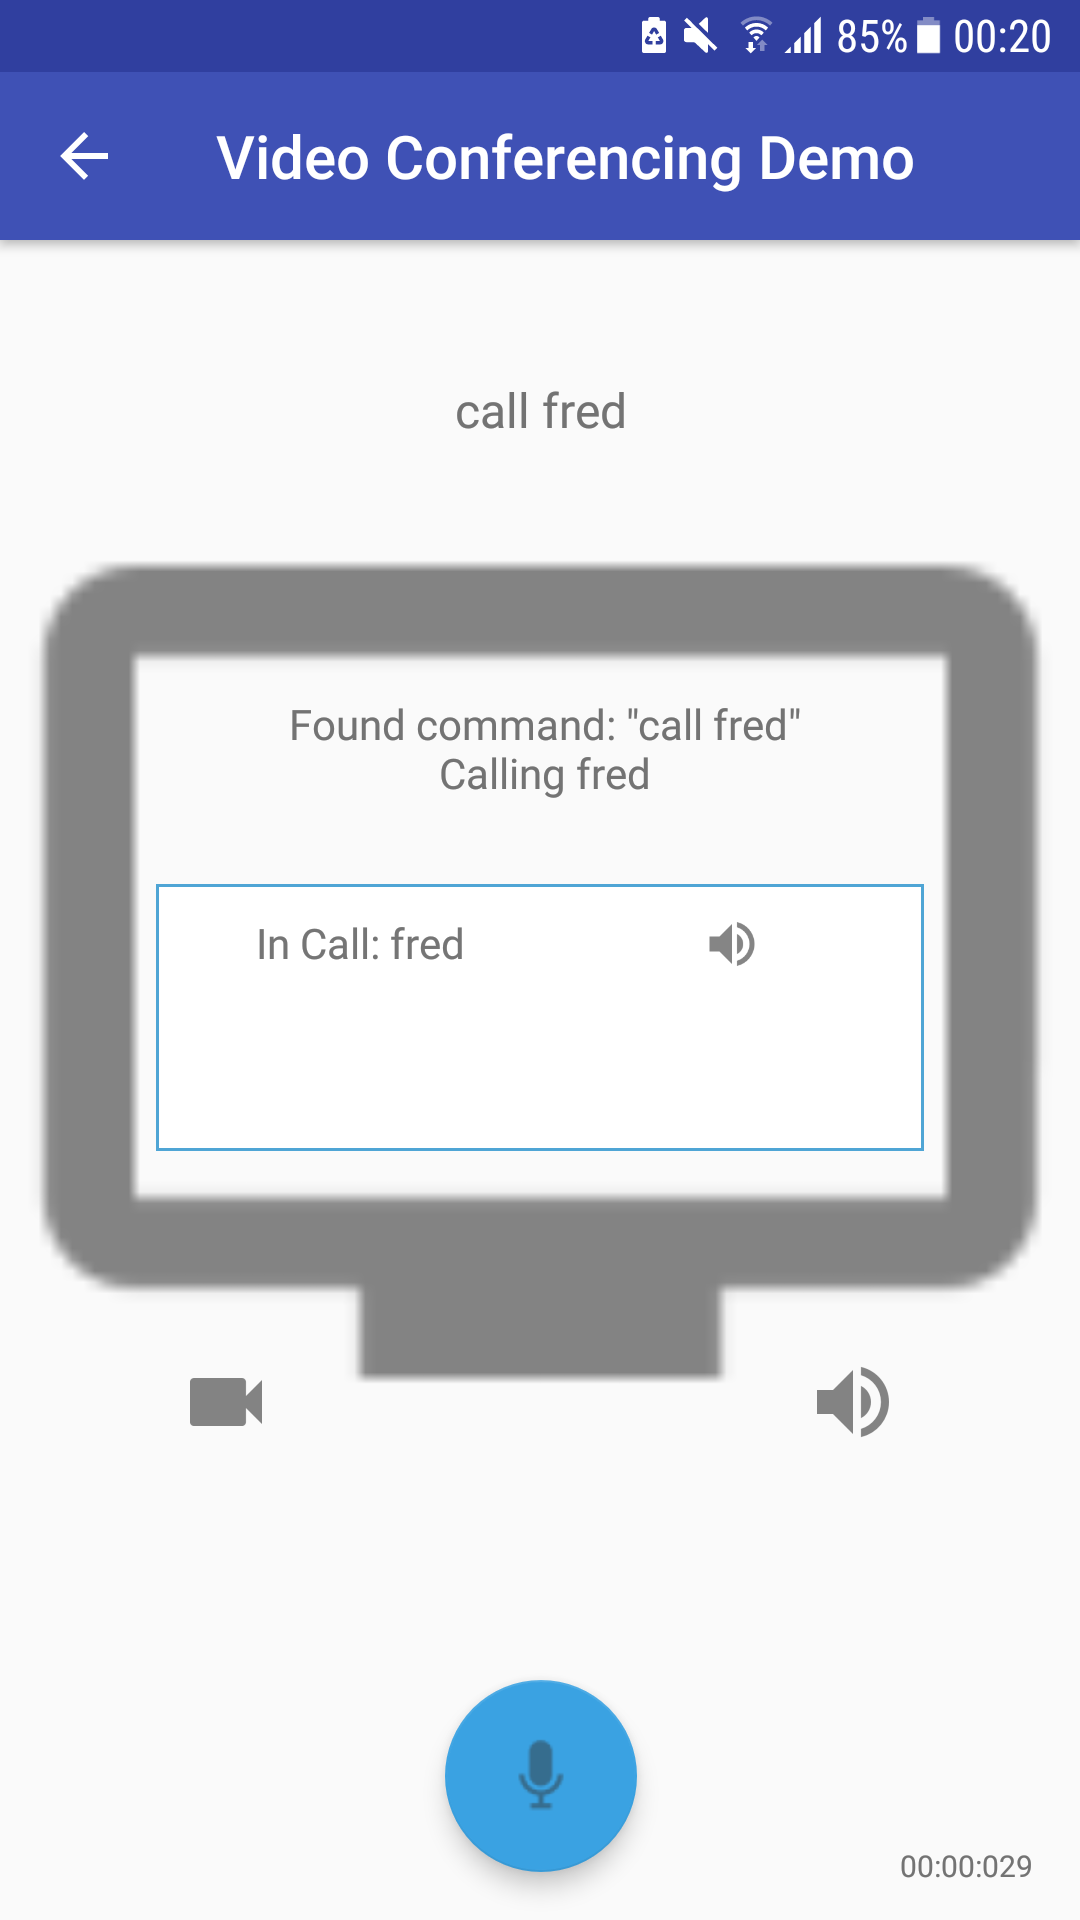
\includegraphics[scale=0.3]{snapshot-calling.png}
  \caption{A screenshot of the user interface for the video conferencing demo.}
  \label{fig:snapshot-calling}
  \end{center}
\end{figure}
\end{center}

The user is able to call a contact and add more contacts to the current call. All participants are displayed on the screen and the user can choose to end a call with a specific person, or end all of the calls. The user can also choose to mute the audio of a certain participant, or mute their own video/audio (with the video/audio icons changing accordingly).
\\
\\
Figure \ref{fig:call-context-action-map} shows the context-action `table' for the video conferencing demo. See the the full \texttt{CallContextActionMap} class in the project's repository. Also see the Appendix \ref{appendix:call-examples} for examples of commands that can be used as well as the list of possible contacts.

\begin{center}
\begin{figure}[H]
\begin{center}
  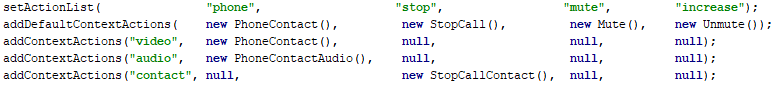
\includegraphics[width=\linewidth]{call-context-action-map.png}
  \caption{A snapshot of the context-action `table' in \texttt{CallContextActionMap.java}.}
  \label{fig:call-context-action-map}
  \end{center}
\end{figure}
\end{center}

The system can also handle duplicate contacts if they exist (e.g. if there are multiple contacts with the first name, ``Fred"). See the Appendix \ref{appendix:duplicate-contacts} for a screenshot of the scenario when an ambiguous contact is called.

\subsection{Settings Activity}
\label{section:settings}

The application also has a settings activity, which allows the user to change various settings such as the current semantic similarity method used, as well as edit the user-defined synonym mappings. See the Appendix \ref{appendix:settings} for a screenshot of the settings activity.

\newpage
\section{Evaluation}
\label{evaluation}

This section outlines a quantitative evaluation of the project's correctness and performance. It also contains a qualitative evaluation of practicality of the voice recognition system and whether it is easy to use via an anonymous survey\footnote{https://goo.gl/forms/8byr4MKo56bqJMvk2}. It should be noted that the results use a small sample size of eight, and are only supplementary to this section.

\subsection{Mock Testing}
\label{section:mock-testing}

Different systems in the Android application are tested for correctness using Android Instrumentation tests and the \textit{Android JUnit} framework. These tests run directly on the Android device without using the GUI; only the individual modules are tested in a closed environment.
\\
\\
There a four test classes in the Android project, each containing several test suites that test certain functionalities (a test suite can have between 3-20 different tests):

\begin{itemize}
\item \texttt{BattleTest.java} | tests the correctness of commands during the \textit{Battle} mode.

\item \texttt{OverworldTest.java} | tests the correctness of commands for the \textit{Overworld} mode.

\item \texttt{CallTest.java} | tests the correctness of video conferencing commands.

\item \texttt{WordNetTest.java} | tests the interaction with the WordNet database; also tests the \texttt{SentenceMapper} class. 
\end{itemize}

Listing \ref{lst:battle-test-inventory} shows an example of a test suite for testing commands that show the inventory in \texttt{BattleTest.java}. Note that some tests actually test for \textit{incorrectness} of a command (such as line 7 of the listing).

\begin{lstlisting}[language=Java, label=lst:battle-test-inventory]
@Test
public void testInventorySuite() {
    gameState.initBattleState(new Troll(9999999));
    gameState.getInventory().add(new Weapon("hammer", "blunt", "heavy"));
    gameState.getInventory().add(new Weapon("sword", "sharp", "metal", "pointy"));
    testInventoryShown("show my inventory", true);
    testInventoryShown("show my troll", false);
    testInventoryShown("show my bag", true);
    testInventoryShown("please show the contents of my possessions that I have", true);
    testInventoryShown("look at my inventory", true);
}
\end{lstlisting}

New tests were added frequently and were executed to ensure a new feature did not break another feature. New features could not be committed to the project's repository unless every test in every test suite of every test class passed with no errors.
\\
\\
See the Appendix \ref{appendix:mock-tests} for a list of commands that are tested for correctness using the mock tests (note that not all tests are shown here). See the project's repository for the entire testing framework.

\subsection{Evaluation of Semantic Similarity}
\label{section:eval-similarity}

The semantic similarity engine | on its own without any helper mechanisms (such as synonym-mapping, sentence-matching, match-ignoring, etc.) | has been evaluated based on the number of different commands that it can detect.
\\
\\
A separate Java project was created that runs the system on a set of commands across three entirely different domains: commands that may be found in a game; video conferencing commands; and commands that may potentially be used in a cooking system/application. On each run, a different semantic similarity method is used.
\\
\\
The number of tests passed for each domain is calculated as a percentage of the total tests, and a final score is calculated for that semantic similarity method (as an average of all three domain scores), with the results saved as a CSV file.
\\
\\
In the evaluation project, the action methods do not perform any function; they simply return a string containing the output (e.g. ``ATTACK\_WEAPON" for attacking with a  sword; ``SERVE\_SOUP" for serving soup, etc.). Each test case is a pair containing a string input (i.e. the user's utterance) and the expected output. For each test case, the string input is used to update the game/calling/cooking state. The output from the object is compared to the expected output, and the results are written to the CSV file. The time taken for a test suite is also recorded, as well as the average time taken for each test.
\\
\\
The \texttt{ContextActionMap}s used in this evaluation project are not the same as the ones used in the Android application (they do not use any helper mechanisms). See the Appendix \ref{appendix:evaluation-context-action-maps} for the context-action mappings used in this evaluation projects.
\\
\\
Tables \ref{table:game-scores}, \ref{table:calling-scores} and \ref{table:cooking-scores} below show the results of the evaluation using the Wu and Palmer (WUP) method.

\begin{table}[]
\centering
\caption{Game Tests}
\label{table:game-scores}
\begin{tabular}{lll}
\multicolumn{1}{l|}{Test}                           & \multicolumn{1}{l|}{Expected}           & Result                       \\ \hline
\multicolumn{1}{l|}{attack}                         & \multicolumn{1}{l|}{ATTACK}             & \cellcolor[HTML]{67FD9A}PASS \\ \hline
\multicolumn{1}{l|}{charge}                         & \multicolumn{1}{l|}{ATTACK}             & \cellcolor[HTML]{67FD9A}PASS \\ \hline
\multicolumn{1}{l|}{hit}                            & \multicolumn{1}{l|}{ATTACK}             & \cellcolor[HTML]{67FD9A}PASS \\ \hline
\multicolumn{1}{l|}{tackle}                         & \multicolumn{1}{l|}{ATTACK}             & \cellcolor[HTML]{67FD9A}PASS \\ \hline
\multicolumn{1}{l|}{fight}                          & \multicolumn{1}{l|}{ATTACK}             & \cellcolor[HTML]{67FD9A}PASS \\ \hline
\multicolumn{1}{l|}{assault}                        & \multicolumn{1}{l|}{ATTACK}             & \cellcolor[HTML]{67FD9A}PASS \\ \hline
\multicolumn{1}{l|}{battle}                         & \multicolumn{1}{l|}{ATTACK}             & \cellcolor[HTML]{67FD9A}PASS \\ \hline
\multicolumn{1}{l|}{launch an assault}              & \multicolumn{1}{l|}{ATTACK}             & \cellcolor[HTML]{67FD9A}PASS \\ \hline
\multicolumn{1}{l|}{attack with a sword}            & \multicolumn{1}{l|}{ATTACK\_WEAPON}     & \cellcolor[HTML]{67FD9A}PASS \\ \hline
\multicolumn{1}{l|}{attack with something sharp}    & \multicolumn{1}{l|}{ATTACK\_WEAPON}     & \cellcolor[HTML]{67FD9A}PASS \\ \hline
\multicolumn{1}{l|}{attack with something pointy}   & \multicolumn{1}{l|}{ATTACK\_WEAPON}     & \cellcolor[HTML]{FD6864}FAIL \\ \hline
\multicolumn{1}{l|}{attack with something long}     & \multicolumn{1}{l|}{ATTACK\_WEAPON}     & \cellcolor[HTML]{FD6864}FAIL \\ \hline
\multicolumn{1}{l|}{attack with something metallic} & \multicolumn{1}{l|}{ATTACK\_WEAPON}     & \cellcolor[HTML]{67FD9A}PASS \\ \hline
\multicolumn{1}{l|}{heal}                           & \multicolumn{1}{l|}{HEAL}               & \cellcolor[HTML]{67FD9A}PASS \\ \hline
\multicolumn{1}{l|}{recover}                        & \multicolumn{1}{l|}{HEAL}               & \cellcolor[HTML]{67FD9A}PASS \\ \hline
\multicolumn{1}{l|}{regenerate}                     & \multicolumn{1}{l|}{HEAL}               & \cellcolor[HTML]{67FD9A}PASS \\ \hline
\multicolumn{1}{l|}{rest}                           & \multicolumn{1}{l|}{HEAL}               & \cellcolor[HTML]{FD6864}FAIL \\ \hline
\multicolumn{1}{l|}{restore}                           & \multicolumn{1}{l|}{HEAL}               & \cellcolor[HTML]{67FD9A}PASS \\ \hline
\multicolumn{1}{l|}{defend}                           & \multicolumn{1}{l|}{DEFEND}               & \cellcolor[HTML]{67FD9A}PASS \\ \hline
\multicolumn{1}{l|}{guard}                           & \multicolumn{1}{l|}{DEFEND}               & \cellcolor[HTML]{67FD9A}PASS \\ \hline
\multicolumn{1}{l|}{safeguard}                           & \multicolumn{1}{l|}{DEFEND}               & \cellcolor[HTML]{FD6864}FAIL \\ \hline
\multicolumn{1}{l|}{shield}                           & \multicolumn{1}{l|}{DEFEND}               & \cellcolor[HTML]{67FD9A}PASS \\ \hline
\multicolumn{1}{l|}{heal with a potion}             & \multicolumn{1}{l|}{HEAL\_POTION}       & \cellcolor[HTML]{67FD9A}PASS \\ \hline
\multicolumn{1}{l|}{heal with an elixer}            & \multicolumn{1}{l|}{HEAL\_POTION}       & \cellcolor[HTML]{FD6864}FAIL \\ \hline
\multicolumn{1}{l|}{heal with an healing drink}     & \multicolumn{1}{l|}{HEAL\_POTION}       & \cellcolor[HTML]{67FD9A}PASS \\ \hline
\multicolumn{1}{l|}{move forwards}                  & \multicolumn{1}{l|}{MOVE\_FORWARDS}     & \cellcolor[HTML]{67FD9A}PASS \\ \hline
\multicolumn{1}{l|}{move straight}                  & \multicolumn{1}{l|}{MOVE\_FORWARDS}     & \cellcolor[HTML]{FD6864}FAIL \\ \hline
\multicolumn{1}{l|}{move backwards}                 & \multicolumn{1}{l|}{MOVE\_BACKWARDS}    & \cellcolor[HTML]{67FD9A}PASS \\ \hline
\multicolumn{1}{l|}{move in reverse}                & \multicolumn{1}{l|}{MOVE\_BACKWARDS}    & \cellcolor[HTML]{FD6864}FAIL \\ \hline
\multicolumn{1}{l|}{move ahead}                     & \multicolumn{1}{l|}{MOVE\_FORWARDS}     & \cellcolor[HTML]{FD6864}FAIL \\ \hline
\multicolumn{1}{l|}{continue forwards}              & \multicolumn{1}{l|}{MOVE\_FORWARDS}     & \cellcolor[HTML]{67FD9A}PASS \\ \hline
\multicolumn{1}{l|}{run forwards}                   & \multicolumn{1}{l|}{MOVE\_FORWARDS}     & \cellcolor[HTML]{67FD9A}PASS \\ \hline
\multicolumn{1}{l|}{dash forwards}                  & \multicolumn{1}{l|}{MOVE\_FORWARDS}     & \cellcolor[HTML]{67FD9A}PASS \\ \hline
\multicolumn{1}{l|}{Score:}                         & \multicolumn{1}{l|}{72.73\%}            &                              \\
\end{tabular}
\end{table}

\begin{table}[H]
\scriptsize
\centering
\caption{Video Conferencing Tests}
\label{table:calling-scores}
\begin{tabular}{lll}
\multicolumn{1}{l|}{Test}                           & \multicolumn{1}{l|}{Expected}           & Result                       \\ \hline
\multicolumn{1}{l|}{phone}                          & \multicolumn{1}{l|}{PHONE}              & \cellcolor[HTML]{67FD9A}PASS \\ \hline
\multicolumn{1}{l|}{phone fred}                     & \multicolumn{1}{l|}{PHONE\_FRED}        & \cellcolor[HTML]{67FD9A}PASS \\ \hline
\multicolumn{1}{l|}{phone jane}                     & \multicolumn{1}{l|}{PHONE\_JANE}        & \cellcolor[HTML]{67FD9A}PASS \\ \hline
\multicolumn{1}{l|}{ring jane}                      & \multicolumn{1}{l|}{PHONE\_JANE}        & \cellcolor[HTML]{67FD9A}PASS \\ \hline
\multicolumn{1}{l|}{phone jane with video}          & \multicolumn{1}{l|}{PHONE\_JANE\_VIDEO} & \cellcolor[HTML]{67FD9A}PASS \\ \hline
\multicolumn{1}{l|}{phone jane with webcam}         & \multicolumn{1}{l|}{PHONE\_JANE\_VIDEO} & \cellcolor[HTML]{67FD9A}PASS \\ \hline
\multicolumn{1}{l|}{use webcam to call jane}        & \multicolumn{1}{l|}{PHONE\_JANE\_VIDEO} & \cellcolor[HTML]{FD6864}FAIL \\ \hline
\multicolumn{1}{l|}{call jane with audio}           & \multicolumn{1}{l|}{PHONE\_JANE\_AUDIO} & \cellcolor[HTML]{67FD9A}PASS \\ \hline
\multicolumn{1}{l|}{phone jane with sound}          & \multicolumn{1}{l|}{PHONE\_JANE\_AUDIO} & \cellcolor[HTML]{67FD9A}PASS \\ \hline
\multicolumn{1}{l|}{contact jane with video}        & \multicolumn{1}{l|}{PHONE\_JANE\_VIDEO} & \cellcolor[HTML]{FD6864}FAIL \\ \hline
\multicolumn{1}{l|}{stop call}                      & \multicolumn{1}{l|}{STOP}               & \cellcolor[HTML]{67FD9A}PASS \\ \hline
\multicolumn{1}{l|}{stop call with fred}            & \multicolumn{1}{l|}{STOP\_FRED}         & \cellcolor[HTML]{67FD9A}PASS \\ \hline
\multicolumn{1}{l|}{end call with fred}             & \multicolumn{1}{l|}{STOP\_FRED}         & \cellcolor[HTML]{67FD9A}PASS \\ \hline
\multicolumn{1}{l|}{close}                          & \multicolumn{1}{l|}{STOP}               & \cellcolor[HTML]{FD6864}FAIL \\ \hline
\multicolumn{1}{l|}{finish call with fred}          & \multicolumn{1}{l|}{STOP\_FRED}         & \cellcolor[HTML]{67FD9A}PASS \\ \hline
\multicolumn{1}{l|}{halt call with fred}            & \multicolumn{1}{l|}{STOP\_FRED}         & \cellcolor[HTML]{67FD9A}PASS \\ \hline
\multicolumn{1}{l|}{mute video}                     & \multicolumn{1}{l|}{MUTE\_VIDEO}        & \cellcolor[HTML]{67FD9A}PASS \\ \hline
\multicolumn{1}{l|}{mute screen}                    & \multicolumn{1}{l|}{MUTE\_VIDEO}        & \cellcolor[HTML]{67FD9A}PASS \\ \hline
\multicolumn{1}{l|}{mute jane}                      & \multicolumn{1}{l|}{MUTE\_JANE}         & \cellcolor[HTML]{67FD9A}PASS \\ \hline
\multicolumn{1}{l|}{silence jane}                   & \multicolumn{1}{l|}{MUTE\_JANE}         & \cellcolor[HTML]{FD6864}FAIL \\ \hline
\multicolumn{1}{l|}{Score:}                         & \multicolumn{1}{l|}{80.00\%}            &                              \\
\end{tabular}
\end{table}


\begin{table}[H]
\scriptsize
\centering
\caption{Cooking Tests}
\label{table:cooking-scores}
\begin{tabular}{lll}
\multicolumn{1}{l|}{Test}                           & \multicolumn{1}{l|}{Expected}           & Result                       \\ \hline
\multicolumn{1}{l|}{make egg}                       & \multicolumn{1}{l|}{MAKE\_EGG}          & \cellcolor[HTML]{67FD9A}PASS \\ \hline
\multicolumn{1}{l|}{make eggs}                      & \multicolumn{1}{l|}{MAKE\_EGG}          & \cellcolor[HTML]{67FD9A}PASS \\ \hline
\multicolumn{1}{l|}{make soup}                      & \multicolumn{1}{l|}{MAKE\_SOUP}         & \cellcolor[HTML]{67FD9A}PASS \\ \hline
\multicolumn{1}{l|}{create soup}                    & \multicolumn{1}{l|}{MAKE\_SOUP}         & \cellcolor[HTML]{67FD9A}PASS \\ \hline
\multicolumn{1}{l|}{produce soup}                   & \multicolumn{1}{l|}{MAKE\_SOUP}         & \cellcolor[HTML]{67FD9A}PASS \\ \hline
\multicolumn{1}{l|}{cook egg}                       & \multicolumn{1}{l|}{MAKE\_EGG}          & \cellcolor[HTML]{67FD9A}PASS \\ \hline
\multicolumn{1}{l|}{make omelette}                  & \multicolumn{1}{l|}{MAKE\_EGG}          & \cellcolor[HTML]{FD6864}FAIL \\ \hline
\multicolumn{1}{l|}{make something liquid}          & \multicolumn{1}{l|}{MAKE\_SOUP}         & \cellcolor[HTML]{FD6864}FAIL \\ \hline
\multicolumn{1}{l|}{boil egg}                       & \multicolumn{1}{l|}{BOIL\_EGG}          & \cellcolor[HTML]{67FD9A}PASS \\ \hline
\multicolumn{1}{l|}{heat egg}                       & \multicolumn{1}{l|}{BOIL\_EGG}          & \cellcolor[HTML]{67FD9A}PASS \\ \hline
\multicolumn{1}{l|}{boil soup with cooker}          & \multicolumn{1}{l|}{BOIL\_SOUP\_COOKER} & \cellcolor[HTML]{67FD9A}PASS \\ \hline
\multicolumn{1}{l|}{boil soup with boiler}          & \multicolumn{1}{l|}{BOIL\_SOUP\_COOKER} & \cellcolor[HTML]{67FD9A}PASS \\ \hline
\multicolumn{1}{l|}{boil soup with stove}           & \multicolumn{1}{l|}{BOIL\_SOUP\_COOKER} & \cellcolor[HTML]{FD6864}FAIL \\ \hline
\multicolumn{1}{l|}{heat pottage with stove}        & \multicolumn{1}{l|}{BOIL\_SOUP\_COOKER} & \cellcolor[HTML]{FD6864}FAIL \\ \hline
\multicolumn{1}{l|}{stir soup}                      & \multicolumn{1}{l|}{STIR\_SOUP}         & \cellcolor[HTML]{67FD9A}PASS \\ \hline
\multicolumn{1}{l|}{mix soup}                       & \multicolumn{1}{l|}{STIR\_SOUP}         & \cellcolor[HTML]{FD6864}FAIL \\ \hline
\multicolumn{1}{l|}{blend soup}                     & \multicolumn{1}{l|}{STIR\_SOUP}         & \cellcolor[HTML]{FD6864}FAIL \\ \hline
\multicolumn{1}{l|}{stir chowder}                   & \multicolumn{1}{l|}{STIR\_SOUP}         & \cellcolor[HTML]{67FD9A}PASS \\ \hline
\multicolumn{1}{l|}{stir pottage}                   & \multicolumn{1}{l|}{STIR\_SOUP}         & \cellcolor[HTML]{67FD9A}PASS \\ \hline
\multicolumn{1}{l|}{stir soup with spoon}           & \multicolumn{1}{l|}{STIR\_SOUP\_SPOON}  & \cellcolor[HTML]{67FD9A}PASS \\ \hline
\multicolumn{1}{l|}{stir soup with cutlery}         & \multicolumn{1}{l|}{STIR\_SOUP\_SPOON}  & \cellcolor[HTML]{67FD9A}PASS \\ \hline
\multicolumn{1}{l|}{stir soup with utensil}         & \multicolumn{1}{l|}{STIR\_SOUP\_SPOON}  & \cellcolor[HTML]{67FD9A}PASS \\ \hline
\multicolumn{1}{l|}{stir soup with tablespoon}      & \multicolumn{1}{l|}{STIR\_SOUP\_SPOON}  & \cellcolor[HTML]{67FD9A}PASS \\ \hline
\multicolumn{1}{l|}{stir soup with teaspoon}        & \multicolumn{1}{l|}{STIR\_SOUP\_SPOON}  & \cellcolor[HTML]{67FD9A}PASS \\ \hline
\multicolumn{1}{l|}{stir soup with soupspoon}       & \multicolumn{1}{l|}{STIR\_SOUP\_SPOON}  & \cellcolor[HTML]{67FD9A}PASS \\ \hline
\multicolumn{1}{l|}{blend chowder using soupspoon}  & \multicolumn{1}{l|}{STIR\_SOUP\_SPOON}  & \cellcolor[HTML]{67FD9A}PASS \\ \hline
\multicolumn{1}{l|}{pour buttermilk}                   & \multicolumn{1}{l|}{POOR\_MILK}         & \cellcolor[HTML]{67FD9A}PASS \\ \hline
\multicolumn{1}{l|}{discharge milk}                   & \multicolumn{1}{l|}{POOR\_MILK}         & \cellcolor[HTML]{FD6864}FAIL \\ \hline
\multicolumn{1}{l|}{present eggs}                   & \multicolumn{1}{l|}{SERVE\_EGG}         & \cellcolor[HTML]{FD6864}FAIL \\ \hline
\multicolumn{1}{l|}{deliver soup}                   & \multicolumn{1}{l|}{SERVE\_SOUP}         & \cellcolor[HTML]{67FD9A}PASS \\ \hline
\multicolumn{1}{l|}{Score:}                         & \multicolumn{1}{l|}{63.33\%}            &                              \\

\end{tabular}
\end{table}

\begin{center}
\textbf{Final Score: 71.08\%}
\end{center}

Note that any failed test cases above can be resolved using helper mechanisms (e.g. synonym-mappings, match-ignores, sentence-matching, etc.), which have been removed from the evaluation project.
\\
\\
Table \ref{table:method-results} below shows the final scores for each semantic similarity method outlined in Section \ref{section:semantic-impl}. To see the full results for each semantic similarity method, see the corresponding CSV results file in the project's repository \footnote{The CSV files can be found in the \texttt{evaluation/evaluation-results} directory of the repository.}.

\begin{table}[H]
\centering
\caption{Evaluation of Similarity Methods}
\label{table:method-results}
\begin{tabular}{l|l|l|l|l}
\textbf{Method} & \textbf{Game Score} & \textbf{Video Call Score} & \textbf{Cooking Score} & \textbf{Final Score} \\ \hline
COS             & 54.54\%             & 55.00\%                     & 43.33\%                & 50.60\%              \\ \hline
FASTLESK        & 36.36\%             & 70.00\%                     & 33.00\%                & 43.37\%              \\ \hline
LCH             & 66.67\%             & \textbf{85.00\%}            & \textbf{70.00\%}       & \textbf{72.29\%}     \\ \hline
LESK            & 54.55\%             & 55.00\%                     & 33.33\%                & 46.99\%              \\ \hline
LIN             & 33.33\%             & 70.00\%                     & 33.33\%                & 42.17\%              \\ \hline
PATH            & 33.33\%             & 70.00\%                     & 33.33\%                & 42.17\%              \\ \hline
RES             & 42.42\%             & 55.00\%                     & 20.00\%                & 37.25\%              \\ \hline
WUP             & \textbf{72.73\%}    & 80.00\%                     & 63.33\%                & 71.08\%               
\end{tabular}
\end{table}

The LCH method has the highest final score, closely followed by the WUP method. However, since the WUP method produced a higher score for the game domain (72.73\% which is much higher than the LCH score of 66.67\%), it was chosen to be the default method used in the role-playing game demo.
\\
\\
The results suggest that path-based methods perform better than methods which use information content or the definitions of the words. This could be because words which are close in proximity in the WordNet database tend to be very similar. The exception to this is the PATH method (i.e. using the reciprocal of the distance between the word nodes in the tree) which performed very poorly with a final score of 42.17\%, perhaps because it is a very simplistic algorithm.
\\
\\
These results also suggest that different methods may perform better under different domains, and there is no optimal method that performs the best under all circumstances. Though it is clear that some methods such as the Resnik (RES) method perform poorly under all three domains, and are not suitable for the system.
\\
\\
It should be noted that the performance of the methods could also be dependent on the confidence thresholds that have been set in \texttt{VoiceProcess.java}; adjusting these thresholds could affect the accuracy of the methods either positively or negatively.

\subsubsection{Combining Similarity Methods}

It is possible to combine two different semantic similarity methods and take the average confidence value when comparing the similarity of two words. The evaluation project also calculates the overall scores for different combinations of methods.
\\
\\
Table \ref{table:hybrid-results} shows the final scores for the best combinations of methods. Note that not all combinations are shown; see the project's repository for every combination's final score.
\\
\begin{table}[]
\centering
\caption{Evaluation of Hybrid Methods}
\label{table:hybrid-results}
\begin{tabular}{l|l|l}
\textbf{Method 1} & \textbf{Method 2} & \textbf{Final Score} \\ \hline
FASTLESK              & LCH               & \textbf{74.70\%}     \\ \hline
LESK               & LCH               & \textbf{74.70\%}              \\ \hline
WUP               & COS              & 73.49\%              \\ \hline
LCH          & PATH               & 72.29\%              \\ \hline
WUP               & LCH          & 71.08\%            
\end{tabular}
\end{table}

The Leacock and Chodorow (LCH) and Wu and Palmer (WUP) methods are involved in almost all of the top combinations (since they also have the highest individual final scores). The best combination is the LCH method with either the LESK method or FASTLESK method, and since the FASTLESK method can be up to 10 times faster than the LESK method (see Section \ref{section:performance} below for performance details), it is the preferred combination.
\\
\\
It should be noted that there is only a slight increase from 72.29\% to 74.70\% when combining the LCH method with the FASTLESK method (as opposed to just using the LCH method on its own), so the improvement in recognition in not large with a hybrid method.

\subsection{Performance of Semantic Similarity Methods}
\label{section:performance}

One user requirement for the system for the voice recognition to be fast and responsive; the user does not want to wait a noticeable amount of time until their voice command has been processed. Therefore, a semantic similarity method which is fast is required.
\\
\\
According, Jakob Nielson of the Nielson Norman Group \cite{RefWorks:128}, there are three main response limits determined by human perceptual abilities that should be noted when optimising application performance:

\begin{itemize}
\item 0.1 seconds | the limit for which the user feels the system is instantaneous.
\item 1.0 seconds | the user will notice the delay, but will feel they are not unduly waiting.
\item 10 seconds | the limit for keeping the user's attention; anything longer requires a progress indicator (e.g. progress bar).
\end{itemize}

Ideally, command processing should be limited to 0.1 seconds, with 1 second being the limit for processing commands involving multiple intents, targets or contexts (e.g. ``attack the troll with a sword and with a hammer and then heal using a potion", as the intent would be broken down and processed separately, so may require more processing time).
\\
\\
Using the evaluation project described in Section \ref{section:eval-similarity} above, the average time taken to process one command was calculated for each semantic similarity method on three different machines. Note that the Java program is single-threaded, so multi-core processors are not fully utilised.

\begin{itemize}
\item Desktop PC
	\begin{itemize}
	\item 4 x Intel Core i5-6600K quad-core CPU @ 3.5 GHz
	\item 8 GB RAM
	\end{itemize}
\item Samsung Galaxy S7 Phone
	\begin{itemize}
	\item 4 x Exynos M1 Mongoose octa-core CPU @ 1.6 GHz \cite{RefWorks:127}
	\item 4 GB RAM
	\end{itemize}
\item Raspberry Pi 3
	\begin{itemize}
	\item 1 x ARMv8 quad-core CPU @ 1.2 GHz \cite{RefWorks:126}
	\item 1 GB RAM
	\end{itemize}
\end{itemize}

Table \ref{table:perf} below shows the average time taken to process a command (in seconds) for different semantic similarity methods, across three machines.\footnote{The LESK method is taken over the average of six commands on the phone, and three commands on the Raspberry Pi, due to time constraints.} See the results in the project's repository for the average times for each domain.

\begin{table}[H]
\centering
\caption{Average Time Taken to Process a Command}
\label{table:perf}
\begin{tabular}{l|l|l|l}
\multirow{2}{*}{\textbf{Method}} & \multicolumn{3}{l}{\textbf{Average Time per Command / s}} \\ \cline{2-4} 
                                 & \textit{PC}   & \textit{Phone}   & \textit{Raspberry Pi}   \\ \hline
COS                              & 0.023         & 0.85             & 6.40                    \\ \hline
FASTLESK                         & 0.012         & 1.5              & 5.00                    \\ \hline
LCH                              & 0.004         & 0.099            & 3.29                    \\ \hline
LESK                             & 1.35          & 280.02           & 2068.81 \\ \hline
LIN                              & 0.009         & 0.29             & 5.19                    \\ \hline
PATH                             & 0.004         & 0.088            & 2.96                    \\ \hline
RES                              & 0.007         & 0.12             & 3.29                    \\ \hline
WUP                              & 0.015         & 0.16             & 5.15                   
\end{tabular}
\end{table}

On the Desktop PC, all methods except the LESK method are below the 0.1 seconds limit, so would all be feasible to use. For the Android phone, only the LCH, PATH, RES and WUP methods are close to, or fall below, the 0.1 seconds limit. Unfortunately, all methods take longer than 0.1 seconds on the Raspberry Pi, but all methods fall below the 10 seconds limit (except LESK). This slow speeds on the Raspberry Pi suggests the system is not suitable for low-power processors, such as embedded systems, or remote robots.
\\
\\
Clearly, the LESK method is not feasible on any machine, with the FASTLESK method being manyfold faster . This suggests that the use of definitions from the meronyms and holonyms of the words to calculate the similarity between two words (and any formatting to remove punctuation from the definitions) is not worthwhile in terms of speed (and given that the accuracy of both methods are very similar as seen in Section \ref{section:eval-similarity}, the FASTLESK method is unanimously the preferred method).
\\
\\
Fortunately, methods which produced high accuracy such as LCH and WUP also have fast performance, so they are ideal methods to use in the application. It should also be noted that multi-threading the system may be to at least double the speed of processing.

\subsection{Evaluation of System Features}

As mentioned previously, the system features mechanisms that the developer can use to improve the recognition of various commands. The following is an evaluation of the effectiveness of the helper mechanisms in increasing the number of commands that the system can process correctly.
\\
\\
The system supports the following features that can be toggled in the \texttt{VoiceProcess} class:

\begin{itemize}
\item Using the semantic similarity engine to detect similar words.
\item An alternative slot-filling grammar, \texttt{\{WITH CONTEXT ACTION TARGET\}}, when needed.
\item Creating a mapping of synonyms to their actions, targets or contexts.
\item Ignoring matches for false similarities between two words.
\item Handling ambiguous intents with a suggestion and confirmation.
\item Performing sentence matching.
\end{itemize}

Using the test cases from the Android mock testing (see the Appendix \ref{appendix:mock-tests} for the list of commands that are tested), the number of tests that pass are calculated while gradually activating more features. It is not possible to test the features separately as some are dependent on others being enabled (e.g. the suggestions mechanism requires the semantic similarity engine to be enabled).
\\
\\
The graph on page \pageref{fig:line-chart-features} shows a cumulative line chart of the number of tests that pass as more features are enabled, starting with no features, followed by adding the semantic similarity engine, and so on. There are a total of 158 tests, and with all features enabled, all of the tests pass.


\begin{center}
\begin{figure}[H]
\begin{center}
  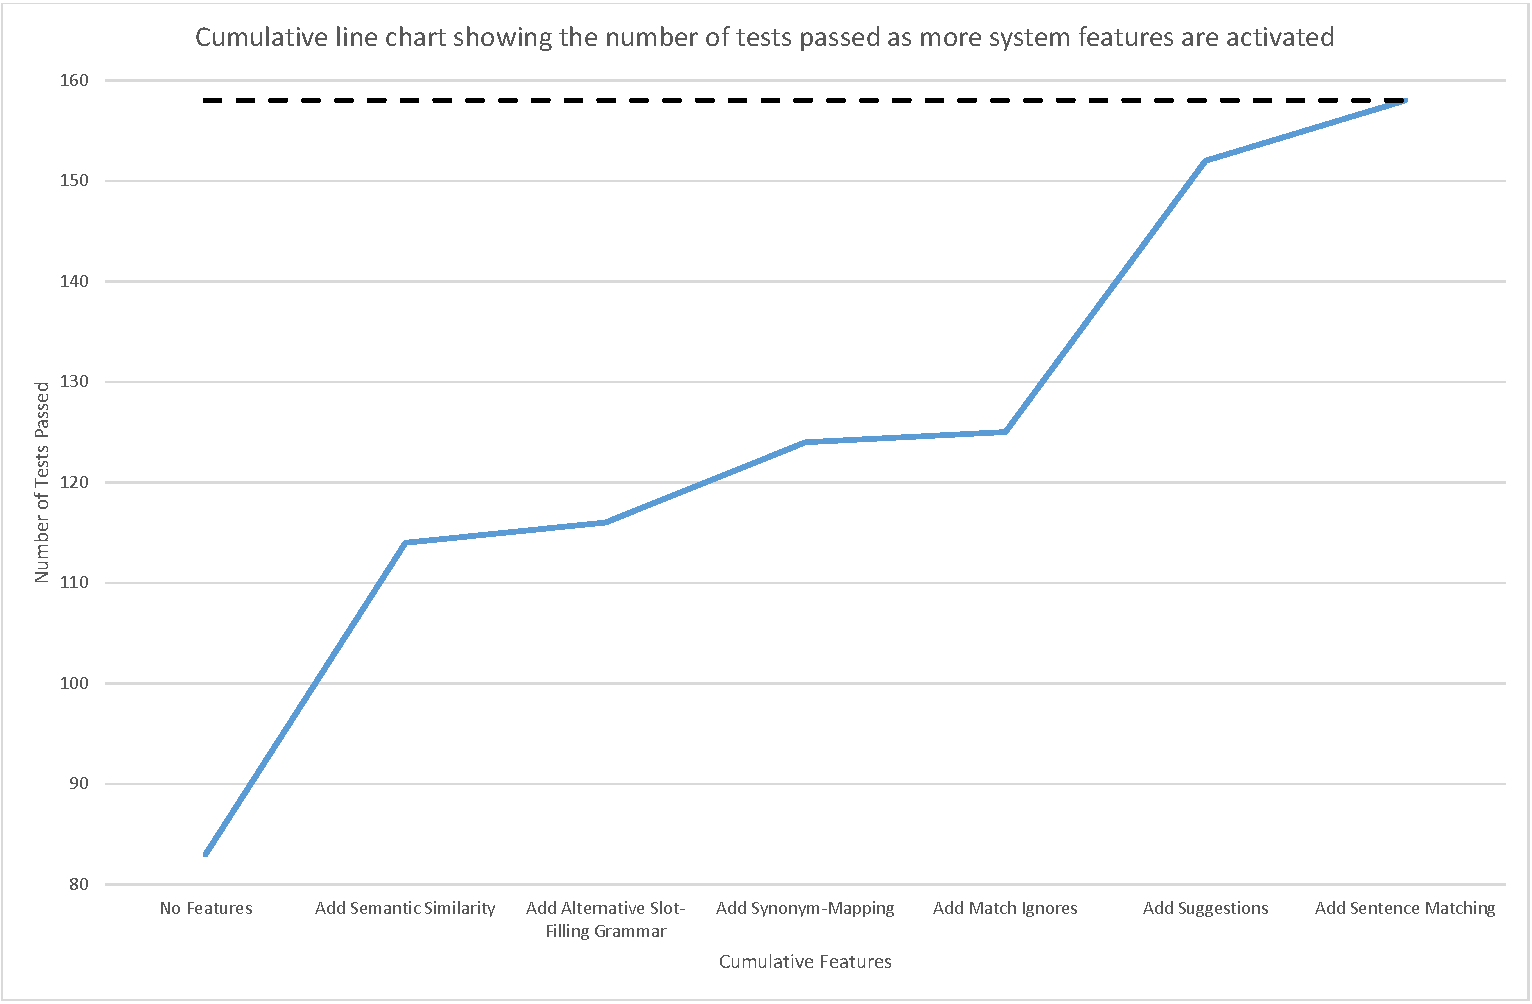
\includegraphics[width=\linewidth]{feature-evaluation.pdf}
  \label{fig:line-chart-features}
  \end{center}
\end{figure}
\end{center}

The large increases in the number of tests that pass when adding the semantic similarity or the suggestions mechanism suggest that have a more sizeable impact compared to the other features. More variations of commands can only be detected if these features are enabled.

\subsection{Evaluation of Slot-Filling Grammar}
\label{section:eval-sfs}

The sentence-matching mechanism was added to compensate for commands that do not have an imperative structure (which is what the current slot-filling grammars detect; see Section \ref{section:slot-filling} on page \pageref{section:slot-filling}). These include intents that are styled as questions, or greetings.
\\
\\
Using the anonymous survey, participants were asked what kind of phrases they would say in a role-playing game. Figure \ref{fig:survey-commands} shows the results for this from eight responses. The question posed was, ``If you were playing a role-playing video game (e.g. Pokemon, Final Fantasy, Elder Scrolls) that supported voice commands, what type of commands are you likely to eventually say?"

\begin{center}
\begin{figure}[]
\begin{center}
  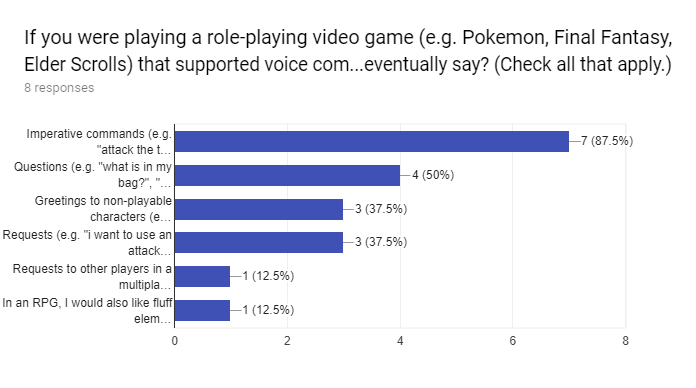
\includegraphics[width=\linewidth]{survey-commands}
  \caption{A bar chart showing the number of users that would eventually say certain types of commands in a role-playing game.}
  \label{fig:survey-commands}
  \end{center}
\end{figure}
\end{center}

While the system covers imperative commands and requests, it does not cover questions and greeting (for which 37.5\% of respondents  would eventually say). Therefore, the sentence-matching mechanism would need to be used to satisfy these users. Unfortunately, since questions and greetings can vary greatly in structure, it is not possible to fit them to a single slot-filling grammar.

\subsection{Usability of the Voice Recognition System}

It is difficult to quantitatively measure how easy it is to use this voice recognition system compared to more traditional methods. One method is to compare the number of lines of code required for a developer to write in order to implement the same number of voice commands in their application.
\\
\\
The voice recognition system implementation will be compared to two na\"ive/traditional systems for adding voice commands to an application.

\begin{description}
\item[Hard-coding Strings] \hfill \\ Adding every possible command as a string and comparing the user's input to them using a series of \texttt{if} and \texttt{else} blocks, or a \texttt{switch} statement.
\item[Regex-style Matching] \hfill \\ Write a word-based regular expression to describe the structure of acceptable commands (see Section \ref{section:houndify} on page \pageref{section:houndify} for an example using Houndify).
\end{description}

When mapping a large number of commands, both of the above methods become increasingly complex and infeasible. With the system presented in this project, only a few lines of code need to be written to map the same number of commands, and more. See the Appendix \ref{appendix:comparison} for a comparison of the methods with an example.
\\
\\
According to the anonymous survey, developers also preferred a system where they only have to write a few lines of code to implement countless voice commands. See the Appendix \ref{appendix:survey-results} for these results.
\\
\\
In order to qualitatively evaluate the usability of the system further, a standalone Java library was created, and the process of using the library in order to add voice commands to a Java application is outlined in a user guide for the library. After studying the guide, developers were asked about the ease of integrating the library into a project via the anonymous survey. Figure \ref{fig:survey-ease} shows the responses to this question.

\begin{center}
\begin{figure}[H]
\begin{center}
  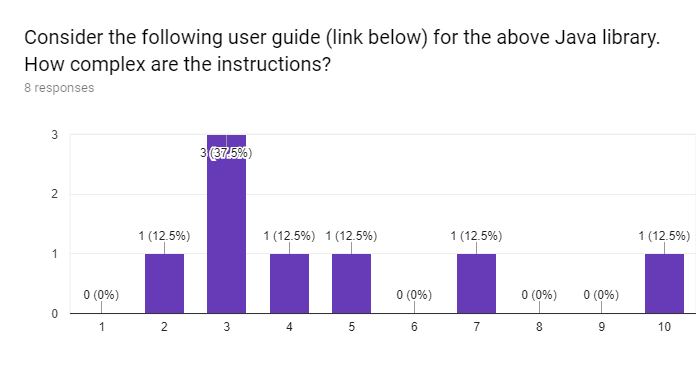
\includegraphics[width=\linewidth]{survey-ease}
  \caption{A bar chart showing the responses for how easy it is to use the voice recognition system in a project on a scale of 1-10, with 1 being ``not complex at all" and 10 being ``extremely complex"}
  \label{fig:survey-ease}
  \end{center}
\end{figure}
\end{center}

Despite the small sample size, the majority of respondents found the system was not that complex to use. However, a couple of respondents found the system to be very complex to use. This could be because the system requires a lot of dependencies and models to be loaded in order to work, or because the

\subsection{Voice Recognition System Limitations}

Several limitations of the voice recognition system were identified over the course of this project, and are described below:

\begin{description}
\item[Only works for Java] \hfill
	\\ The system relies heavily on OOP inheritance, as well as Java-based libraries such as JWI and WS4J. While it may be possible to port the system to another language, it would require a lot of work and re-writing of the source code.
\item[Cannot handle negatives in intents] \hfill
	\\ The system currently cannot handle negatives in a user's utterance. For example, in the video conferencing example, if the user says, ``call Dan with no audio", the ``no" will be ignored and the system will create a call with Dan using audio. It may be possible to fix this by searching for any negatives and altering the intent as needed, but due to time constraints this could not be implemented and tested.
\item[Only single-word actions, targets and contexts are allowed] \hfill
	\\ The voice recognition system scans the input word-by-word, searching for the action, target and context (if they exist). Therefore, it currently cannot identify open compound words such as ``ice cream" or ``full moon", or hyphenated compound words such as ``well-being", ``merry-go-round" or ``on-site" \cite{RefWorks:129}. It may be possible to fix this by implementing a lookahead mechanism which looks at the next word in the input and decides whether it is part of the current word.
	
	This also includes instances where two words are used to describe an action. For example, in the phrase, ``take a look around", the word, ``take" will map to the ``grab" action first, so the system thinks the player wants to grab the surroundings which is not correct.
\item[Not designed for many different targets per action] \hfill
	\\ The use of a \texttt{ContextActionMap} is to handle many different contexts that the action can be performed with. For example, an attack using a blunt weapon may crush the enemy, but an attack from a sharp weapon may slice the enemy. However, in situations where an action is applied differently to many different types of targets, a large block of \texttt{if} and \texttt{else} statements or a \texttt{switch} statement is required to perform different things for different targets within an \texttt{Action} class (e.g. writing a series of \texttt{if (currentTarget instanceof ...) \{...\} else if ...}).
	
	This may be resolved by having a \texttt{TargetActionMap} instead of a \texttt{ContextActionMap}, which indexes the `table' using the target `type' instead. However, this would mean that the same issue will occur when having multiple contexts perform different actions (unless both a \texttt{TargetActionMap} and a \texttt{ContextActionMap} can be used together).
\item[Actions cannot have the same string as target] \hfill
	\\ There is a bug where an action cannot have the same name as a target, as the system becomes confused when parsing and may think the target is actually the action (if the word for the target is a better match than the word of the action in the input).
	
	For example, in the video conferencing example, there may be two actions, ``call" and ``stop". If the user intent is, ``finish the call" where ``call" is the target entity, the system will think that ``call" is a better match to the ``call" action than ``finish" is to the ``stop" action, and will invoke the ``call" action instead. This can easily be fixed by checking the ordering of the matches to see if the action precedes the target.
\item[Cannot handle fully ambiguous inputs] \hfill
	\\ This occurs when a user's intent can be mapped to two completely different actions in the application and both would be valid due to the ambiguity of the intent. For instance, take the phrase, ``throw the match": it could refer to giving up in a competitive competition, or throwing a matchstick.
\end{description}

Many of these limitations are quite severe and hamper the usability of the system under certain circumstances, particularly the restriction to single-word actions, targets and contexts, which would mean actions such as, ``show off" or ``show up" cannot be disambiguated. However, many are relatively easy fixes, and almost all of them could be fixed over time, without breaking any existing functionality.

\subsection{Room Generation Evaluation}

Since the semantic similarity engine used in the room generation program has already been evaluated above, only the effectiveness of the object relationship mechanism needs to be evaluated. This can be done by creating a complex description of a room with all but the first sentence containing a different relation between two objects, and seeing if the system detects the relationship. See the Appendix \ref{appendix:room-generation-results} for the full results.
\\
\\
While the program can detect relations in sentences such as, ``A letter sits upon the table" or, ``A potion is underneath the table", it cannot detect some simple relations such as, ``There is a chair under the table" or ``A fork lays on the table". This could be because the \textit{Reverb} library does not understand the relations, ``lays on" and ``under". However, the majority of relations are detected by the program, and only a few conditionals have to be added manually by the developer.
\\
\\
The room generation structure currently cannot handle multiple objects being created in the same sentence, so only one object creation can be associated to each sentence in the room description.



\newpage
\section{Conclusion}

This section summarises the findings of this report, as well as the deliverables and contributions of this project. The project work can be found in the main repository \footnote{https://github.com/BaronKhan/VoiceRecognitionRPG}.

\subsection{Deliverables}
\label{section:deliverables}

A prototype for a text-based role-playing game has been created on Android which uses the new voice recognition system to process commands, and is available to download \footnote{https://play.google.com/store/apps/details?id=com.khan.baron.voicerecrpg}. The system makes it easier for developers to detect a wide variety of commands without the developer needing to hard-code any of the phrases (or specify the structure of acceptable phrases); they only have to create the table of context-action mappings, and use the system features, to process commands.
\\
\\
Unlike paid voice recognition services such as IBM's Watson Conversation, Houndify or DialogFlow, this project's voice recognition system is able to work completely offline (and therefore protects the user's privacy) and the processing time per command on an Android device is within an acceptable limit (close to 0.1 seconds).
\\
\\
While there are some limitations to the system, using the WordNet database to calculate semantic similarities between words has produced a working foundation for the system that can be improved, and the system has been applied to other domains such as a video conferencing application.
\\
\\
A separate standalone Java library has been created for the voice recognition system that is open-source for developers to explore, called \textit{Voice Commands with WordNet} \footnote{https://github.com/BaronKhan/voice-commands-with-wordnet}. It includes a user guide explaining how to integrate the library into other Java projects.

\subsection{Contributions}
\label{section:contributions}

This project also explored and evaluated different semantic similarity methods in terms of accuracy and performance, with path-based methods such as the Leacock and Chodorow (LCH), and Wu an Palmer (WUP) methods performing the best.
\\
\\
A new interface for the WS4J library was created which uses MIT's JWI API to access the WordNet database \footnote{https://gist.github.com/BaronKhan/5679157d1a8572debc8c75af1c875c16}. This interface has been made public and may be useful to other developers in the future.
\\
\\
Finally, the semantic similarity engine created for the voice recognition system has also been applied to other areas of development for the RPG. For instance, a room generation program has been created which takes as input a text description of the room, and generates a source file for the room, making it easier to create more complex rooms for the game.
\\
\\
Ideas and techniques used in the room generation program, such as identifying binary relationships between objects and using the semantic similarity engine for object creation, may be useful for other systems and projects.

\subsection{Future Work}

This section outlines any future work that may be done as a result of the work already done in this project.

\subsubsection{Language Support}

The voice recognition system components | from the slot-filling grammar structure to the WordNet database | only work for the English language, and will need to be adjusted for other languages.
\\
\\
While approximately 42\% of the world's language use a \textit{subject-verb-object} sentence structure (e.g. ``He hits the goblin"), such as English, Mandarin and Spanish, approximately 45\% of languages use a \textit{subject-object-verb} sentence structure (e.g. ``He the goblin hits"), such as Bengali, Greek and Japanese \cite{RefWorks:130}. Therefore, the target would precede the object, so the voice recognition system's slot-filling grammar needs to be rearranged.
\\
\\
The Princeton University WordNet database only supports English words. While there are WordNet databases for most of the world's languages \cite{RefWorks:131}, each database requires a new interface to be implemented (although most of them are SQL databases which can be queried), and not all languages have a WordNet database currently.

\subsubsection{Deep Learning}

This project has used classical natural language processing techniques, but it may be possible to use deep learning to improve the accuracy and usability of the voice recognition system, such as using recurrent neural networks (RNN). While deep learning requires a large amount of processing and would not be feasible to train offline, models can be trained by the developer and included in the application, with updates to the model included with updates to the application or game.
\\
\\
One use for deep learning is to be able to choose the most appropriate semantic similarity methods to use for a specific domain. As shown in Section \ref{section:performance} on page \pageref{section:eval-similarity}, different methods perform better for different domains. Currently, only a combination of upto two methods can used, with each method having a 50\% weighting. Using deep learning, the best weightings for several methods can be trained to produce the most accurate and best performing combination.
\\
\\
Another area where deep learning (or classical machine learning) techniques can be used is the suggestions mechanism. A global model can be trained whenever an ambiguous intent is spoken, so that the system learns that the user meant another intent instantly (instead of constantly asking them for confirmation of their intent).


\subsubsection{Multi-threading}

During this project, an attempt to multi-thread the application was made, but was unable to achieve a sizeable improvement in performance. Multiple processors could be used to fork and join tasks instead of executing them sequentially. This can be achieved using Java 8's parallel streams \cite{RefWorks:132}.
\\
\\
For example, in the \texttt{SentenceMapper} class, instead of iterating through a \texttt{Collection} of \texttt{sentences} to calculate their cosine similarity score, and then reducing the output sequentially:

\begin{lstlisting}[language=Java, label=lst:loop-seq]
for (String sentence : sentences) {
    totalScore += calculateCosScore(words, sentence);
}
\end{lstlisting}

A parallel stream can be used instead:

\begin{lstlisting}[language=Java, label=lst:loop-stream]
totalScore = sentences.parallelStream()
        .mapToDouble((sentence) -> calculateCosScore(words, sentence))
        .sum();
\end{lstlisting}

Most of the multi-threading can be performed in the \texttt{VoiceProcess} class, where words are currently processed sequentially, although a lot of re-factoring is required to make loop iterations independent within the class.

\subsubsection{Hands-Free UI}

One of the novelties of voice controls is that the user doesn't have to touch any physical buttons or screens in order to execute commands in the application. The interface of the role-playing game in this project requires the player to push a blue button in order to start a voice intent.
\\
\\
It may be possible to replace the button with a wake word detection mechanism. This is a phrase that the user says to indicate the start of a voice intent (such as saying, ``Hi Siri" or ``Ok, Google"). This requires the microphone to always be listening and consume more power, but it will work offline and there are open-source APIs available that offer this, such as \textit{Snowboy} \cite{RefWorks:133}.
\\
\\
It is also possible to turn the output text into audio, using text-to-speech (TTS) API such as Google's TTS engine. Combining these two features would make the application completely hands-free, and could be beneficial to some players.











































































































\newpage
\begin{appendices}
\section{Android Application Screenshots}
This section contains snapshots of the Android application during different scenarios.
\label{appendix:screenshots}
\subsection{Battle Mode Example}
\label{appendix:battle-mode-screenshots}
Below are screenshots of actions performed as the player battles a troll enemy.

\begin{center}
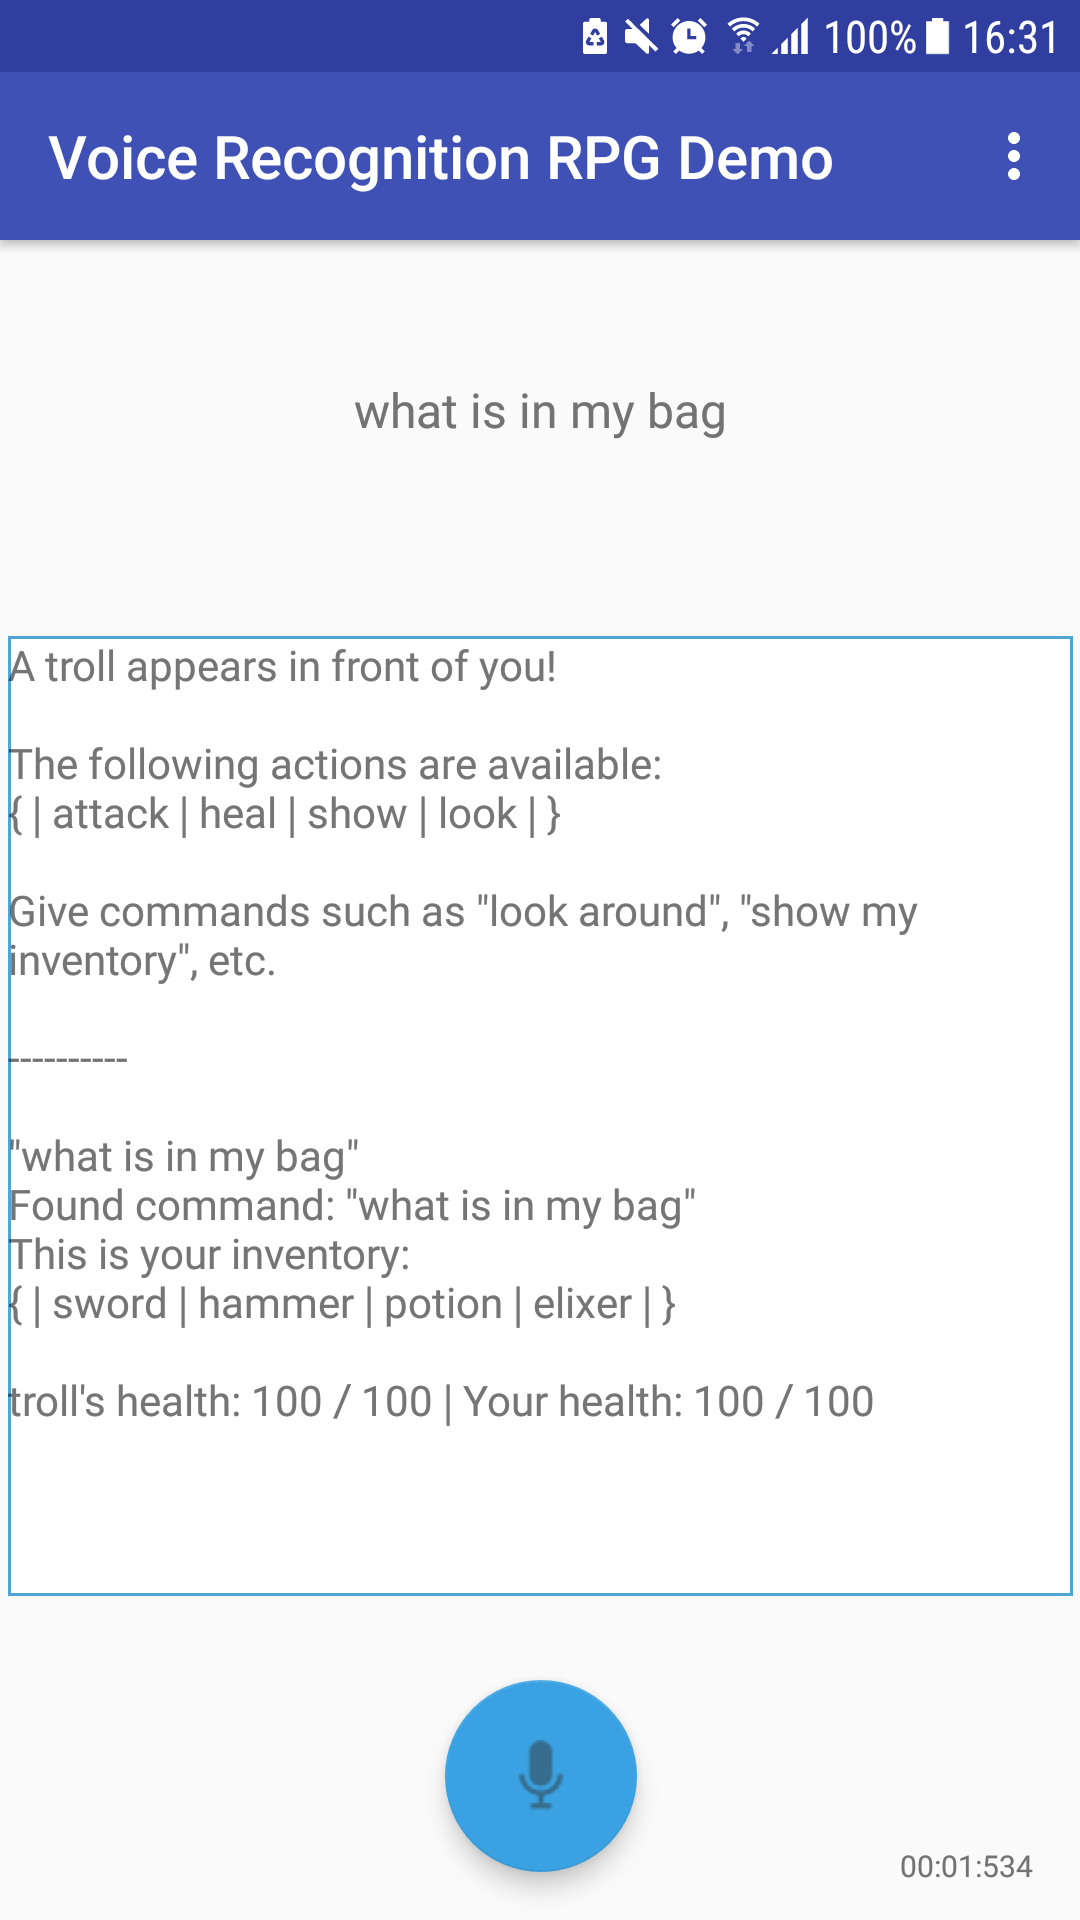
\includegraphics[scale=0.18]{battle-1.png}
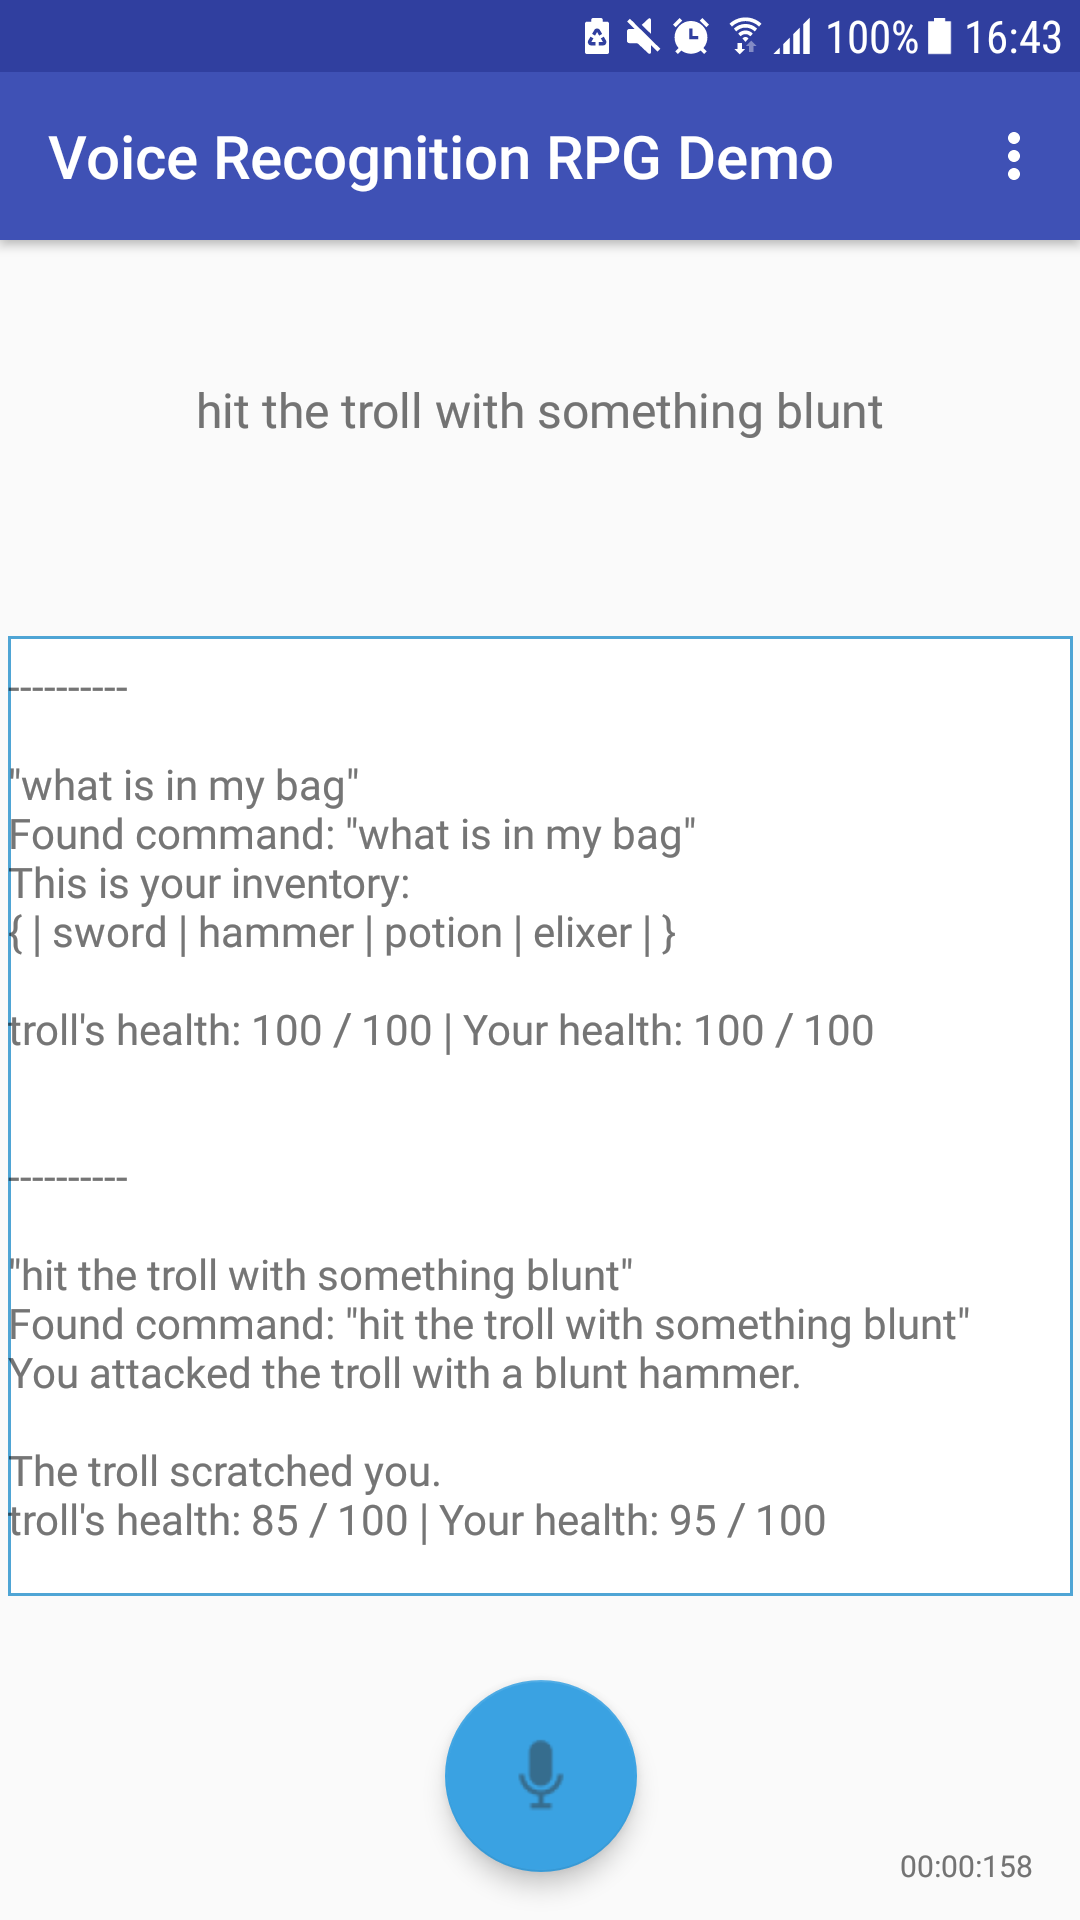
\includegraphics[scale=0.18]{battle-2.png}
\newpage
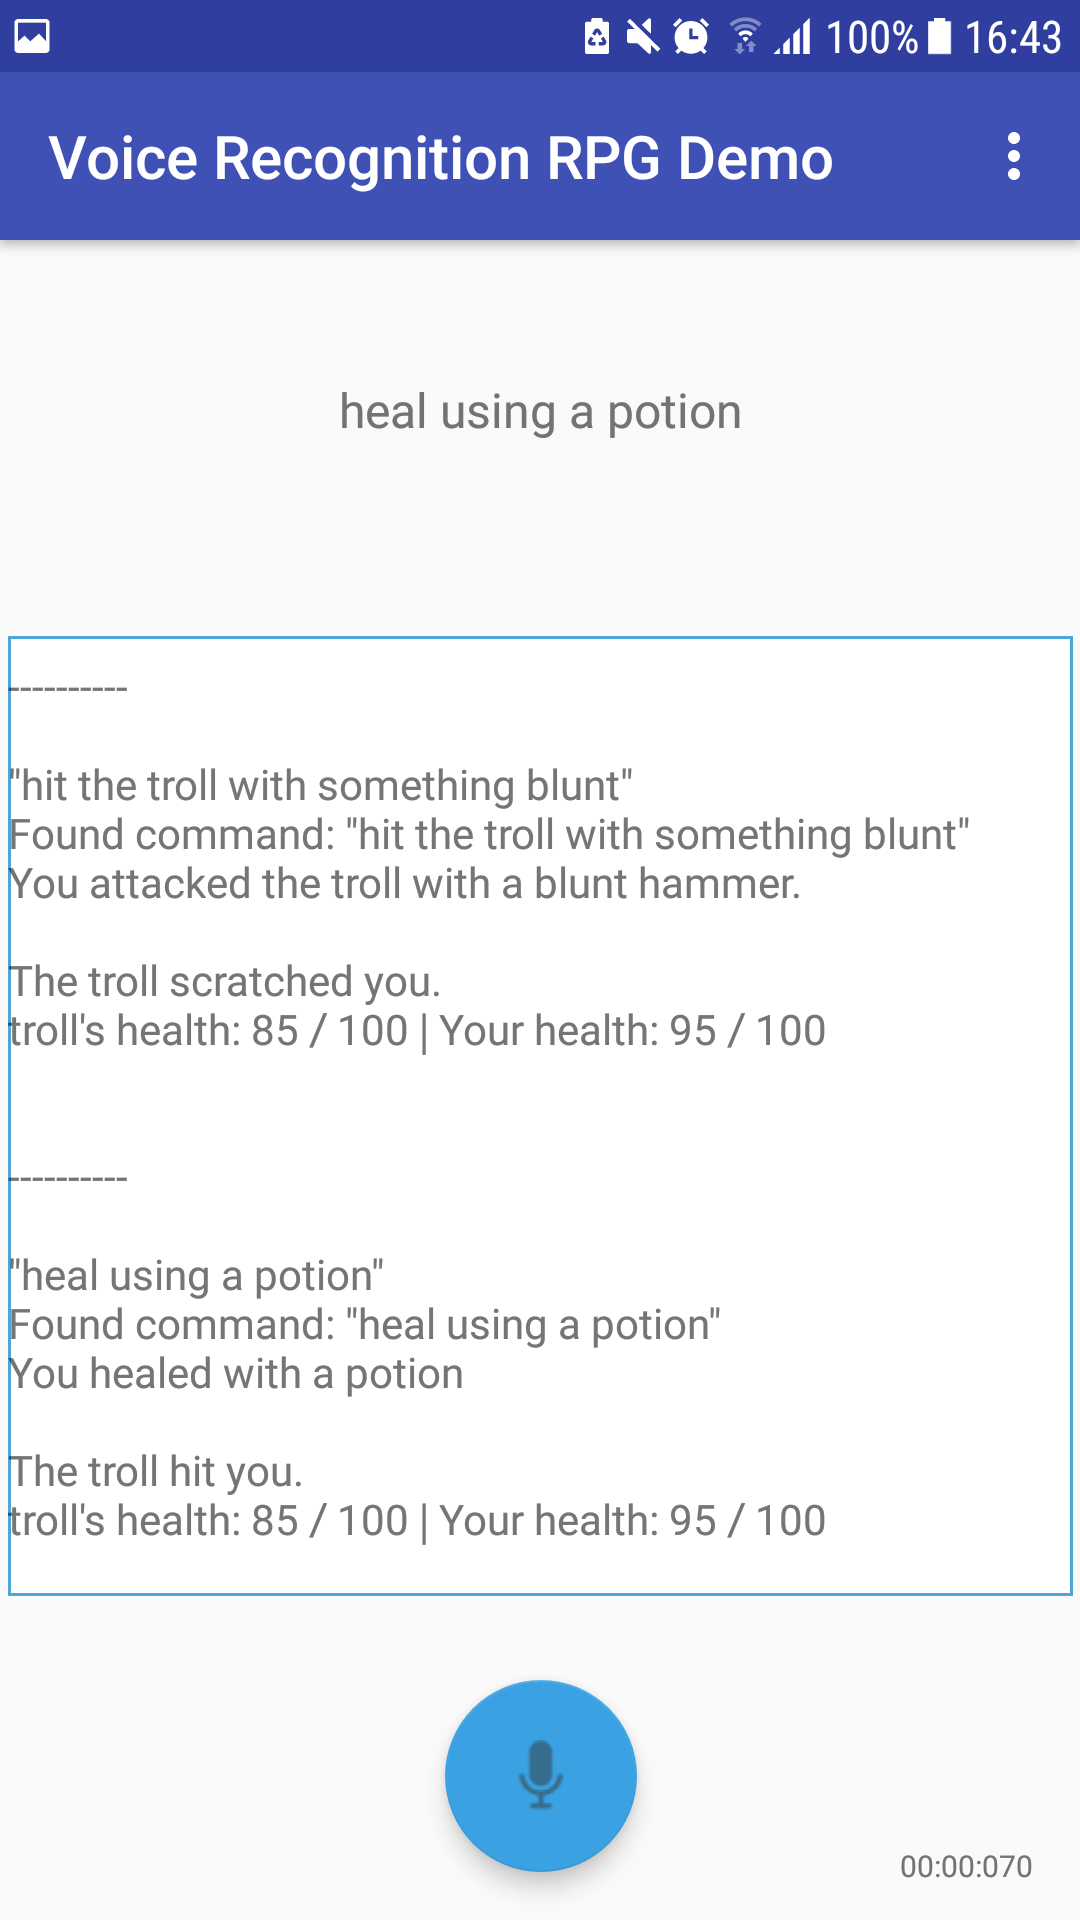
\includegraphics[scale=0.18]{battle-3.png}
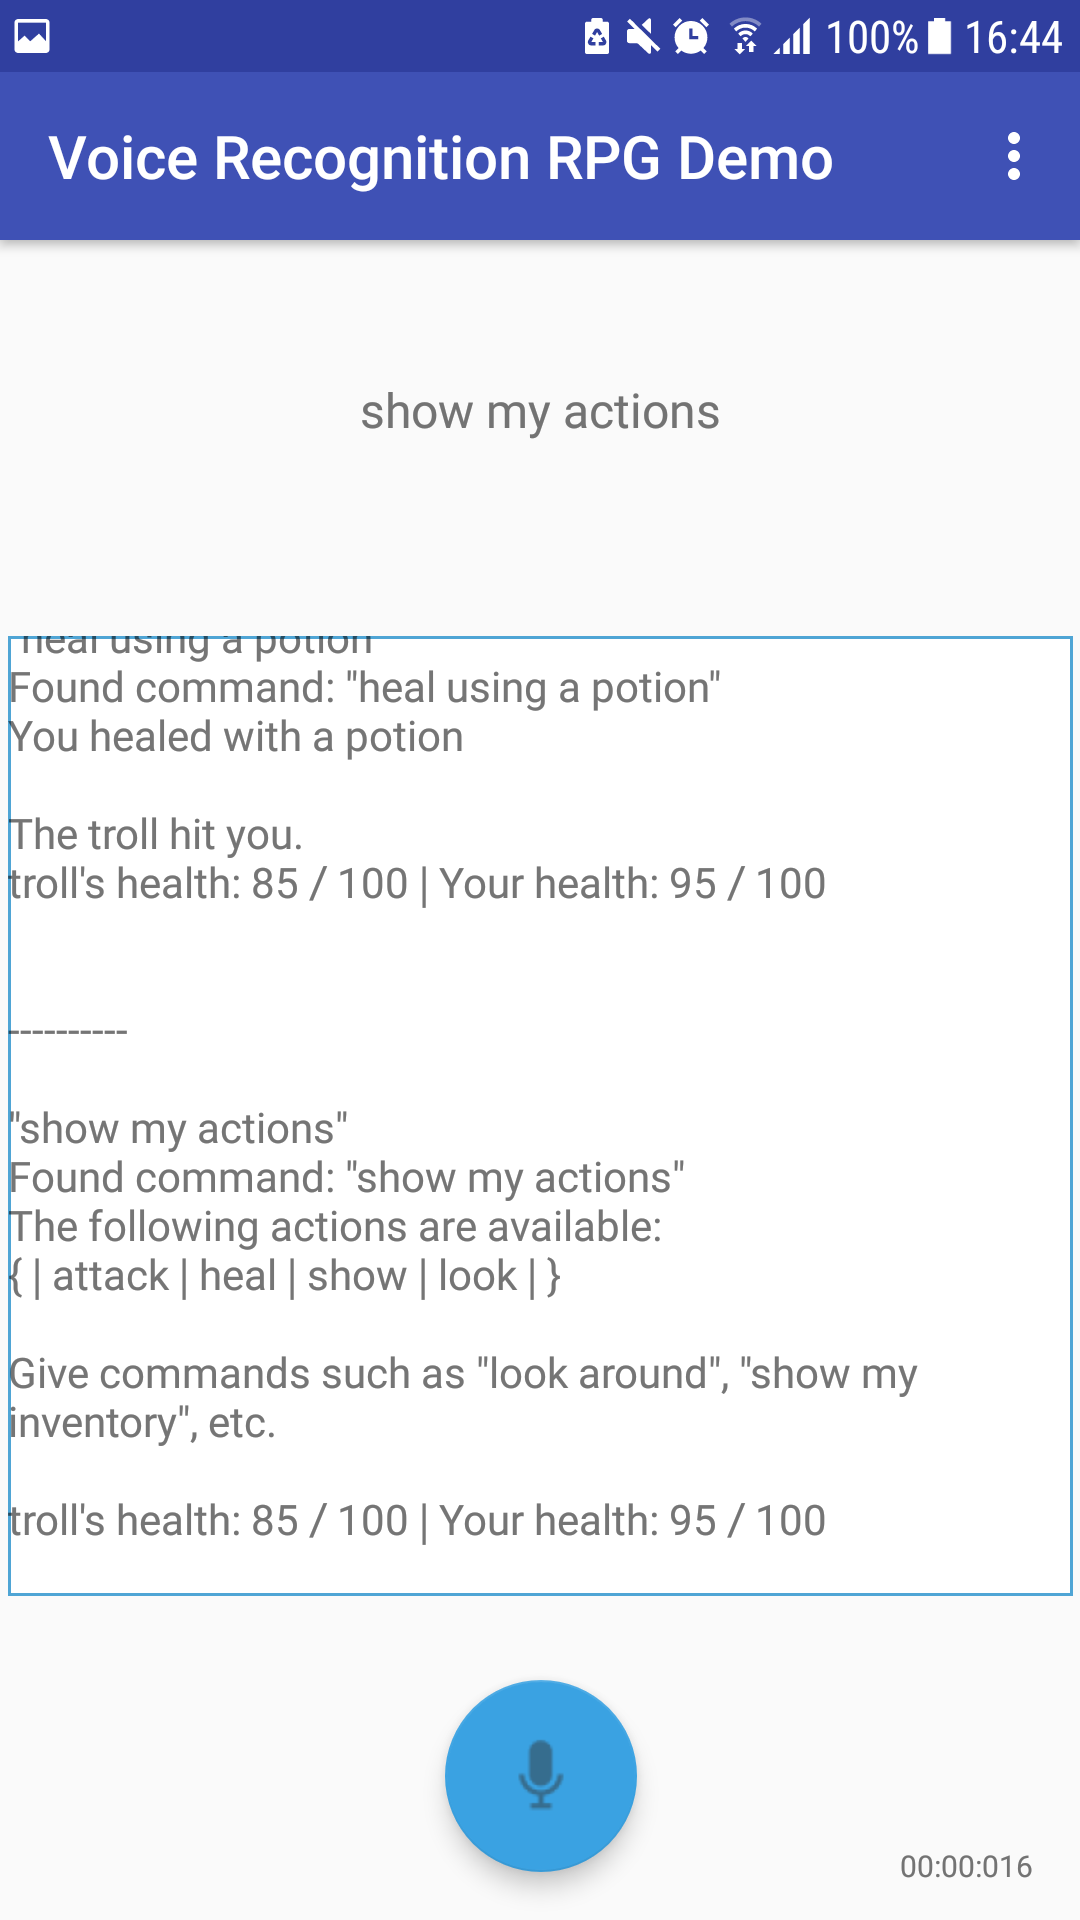
\includegraphics[scale=0.18]{battle-4.png}
\end{center}

\newpage
\subsection{Overworld Mode Example}
\label{appendix:overworld-mode-screenshots}
Below are screenshots of the first room in the game, and the actions required to solve the puzzle in the room.

\begin{center}
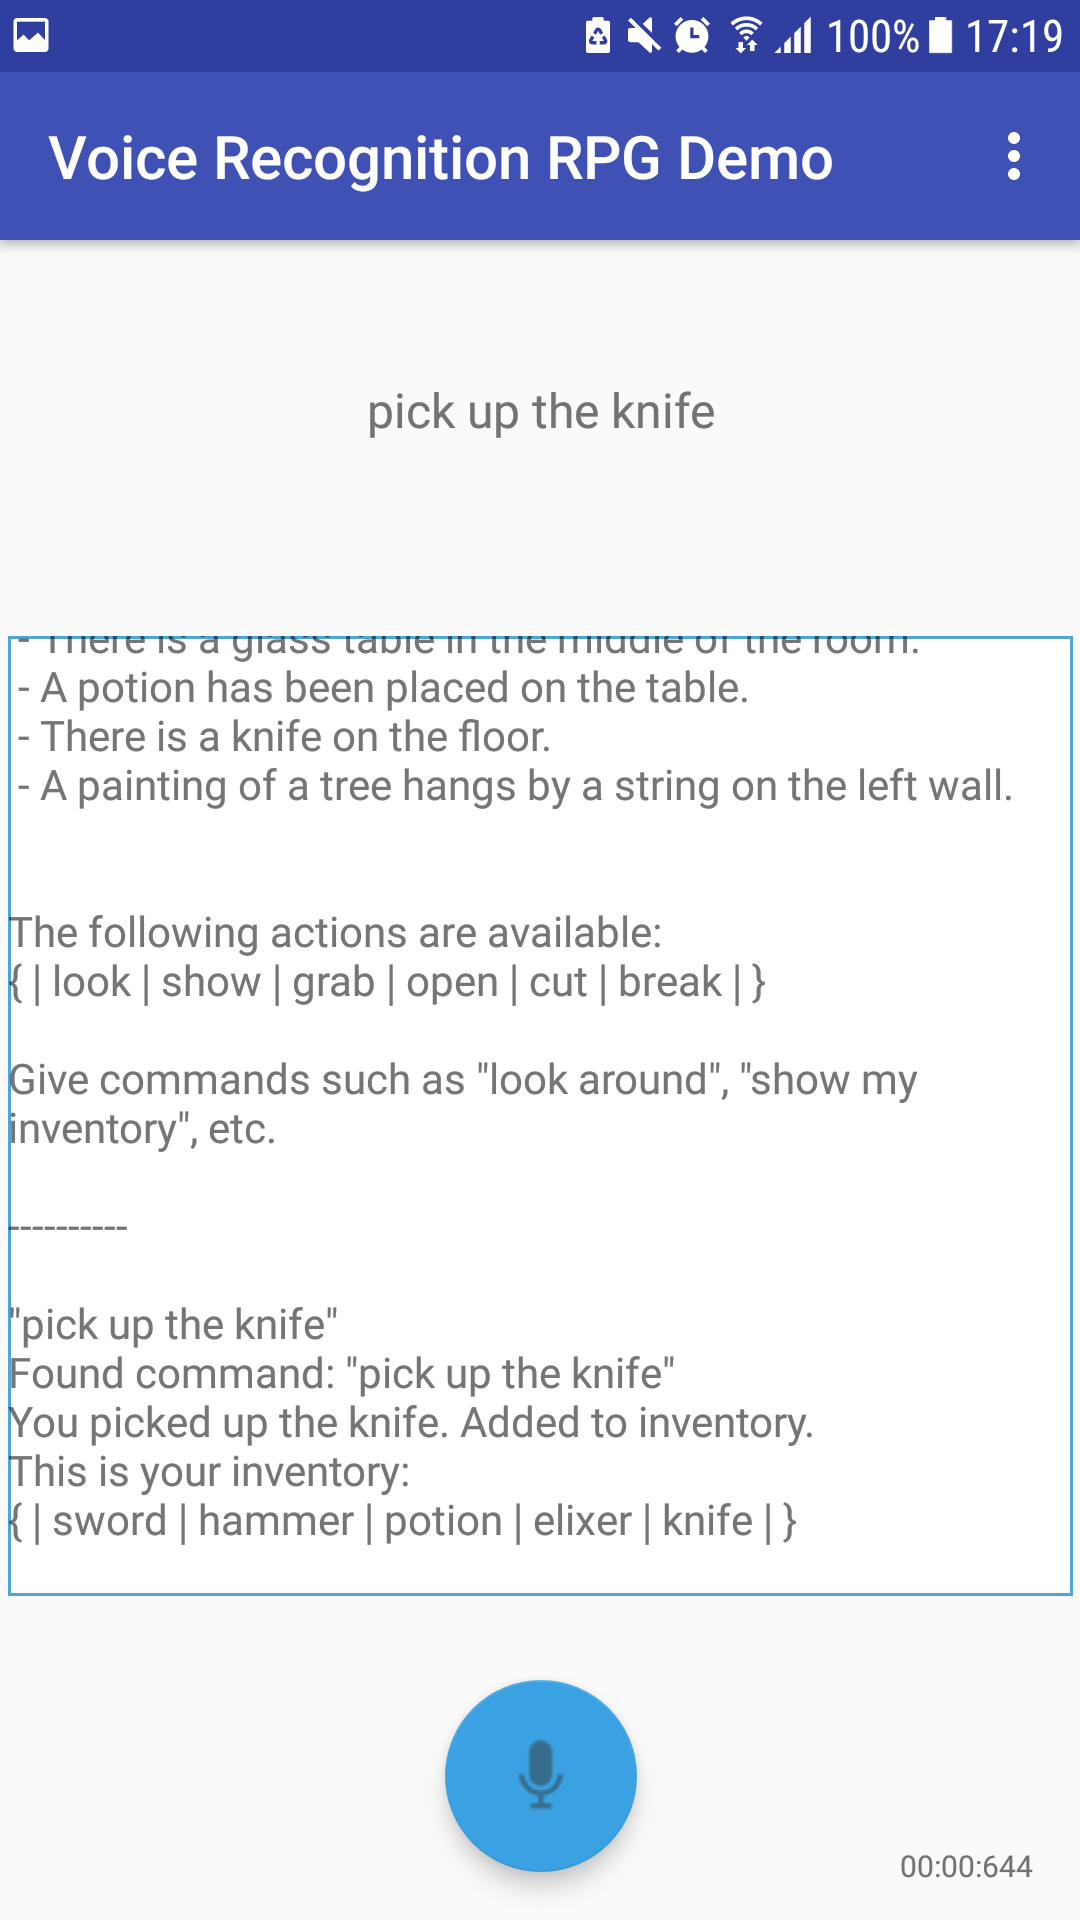
\includegraphics[scale=0.18]{overworld-1.png}
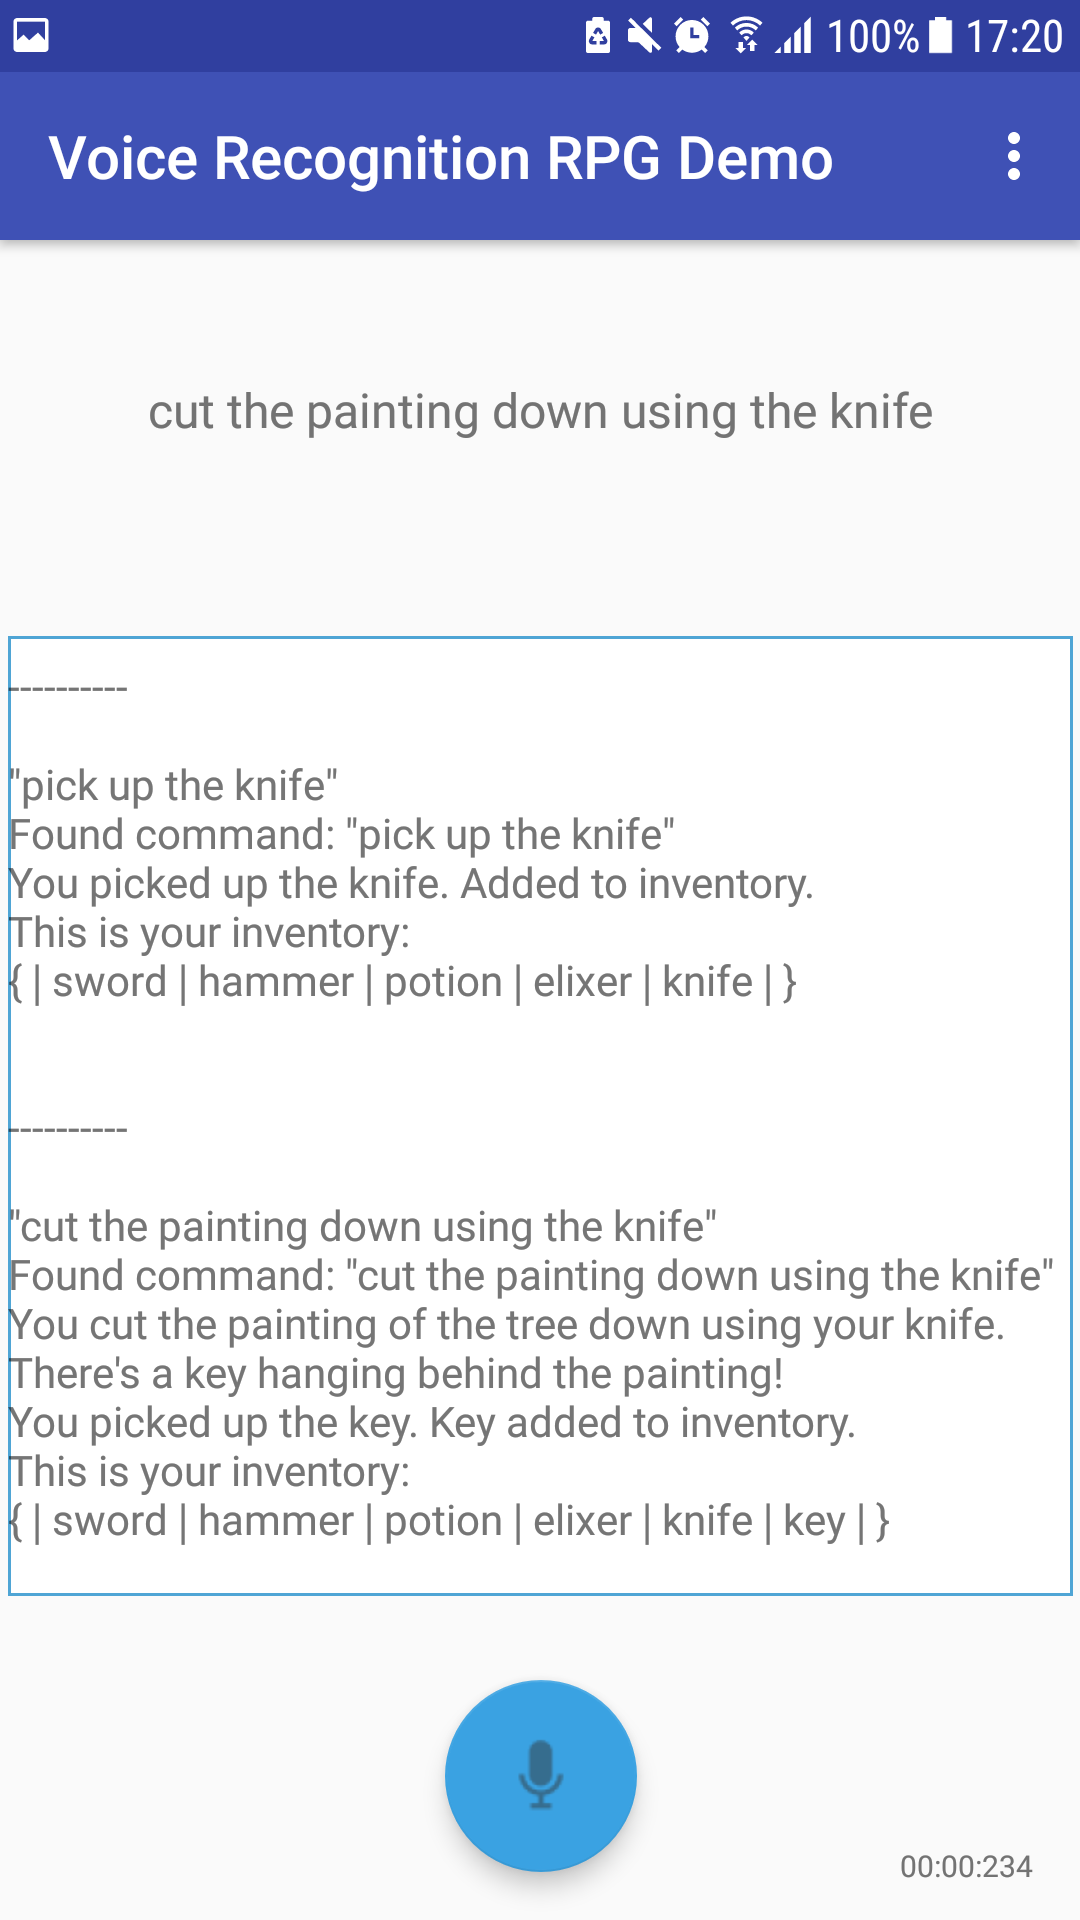
\includegraphics[scale=0.18]{overworld-2.png}
\newpage
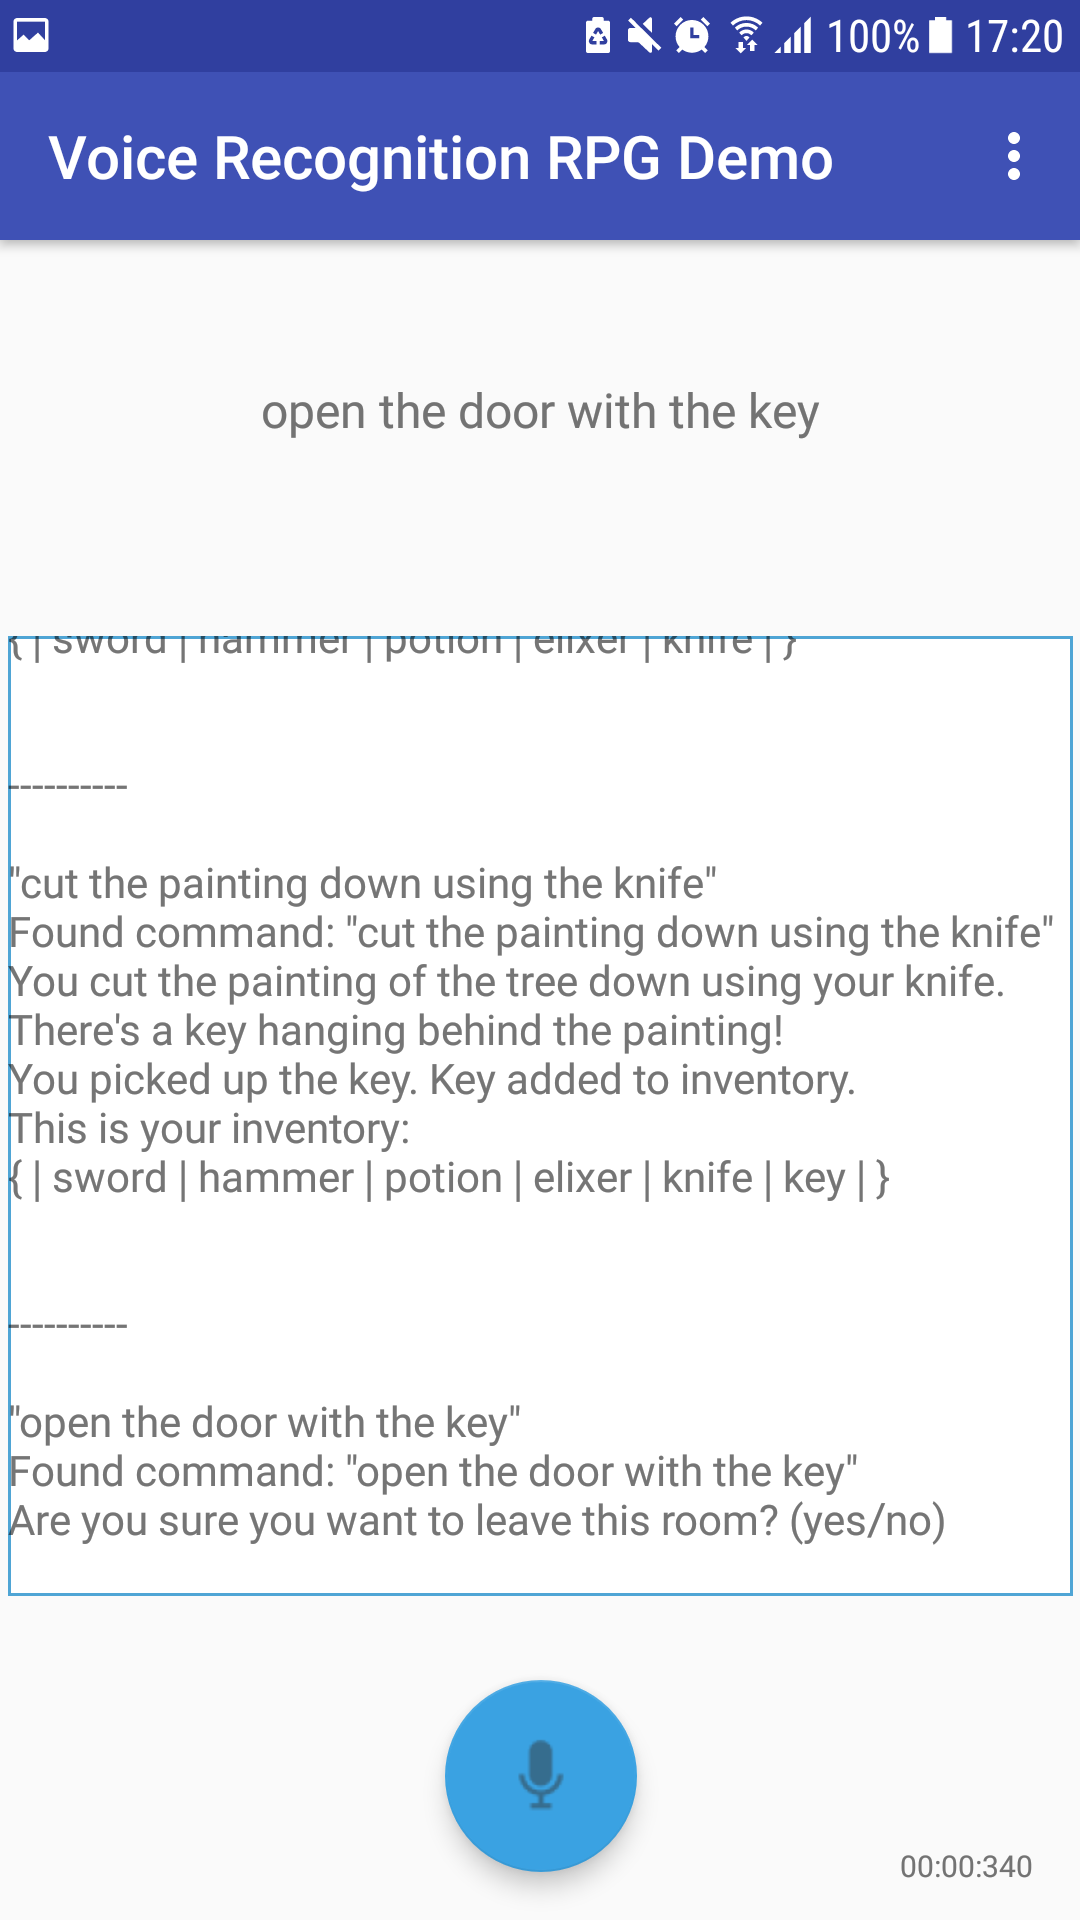
\includegraphics[scale=0.18]{overworld-3.png}
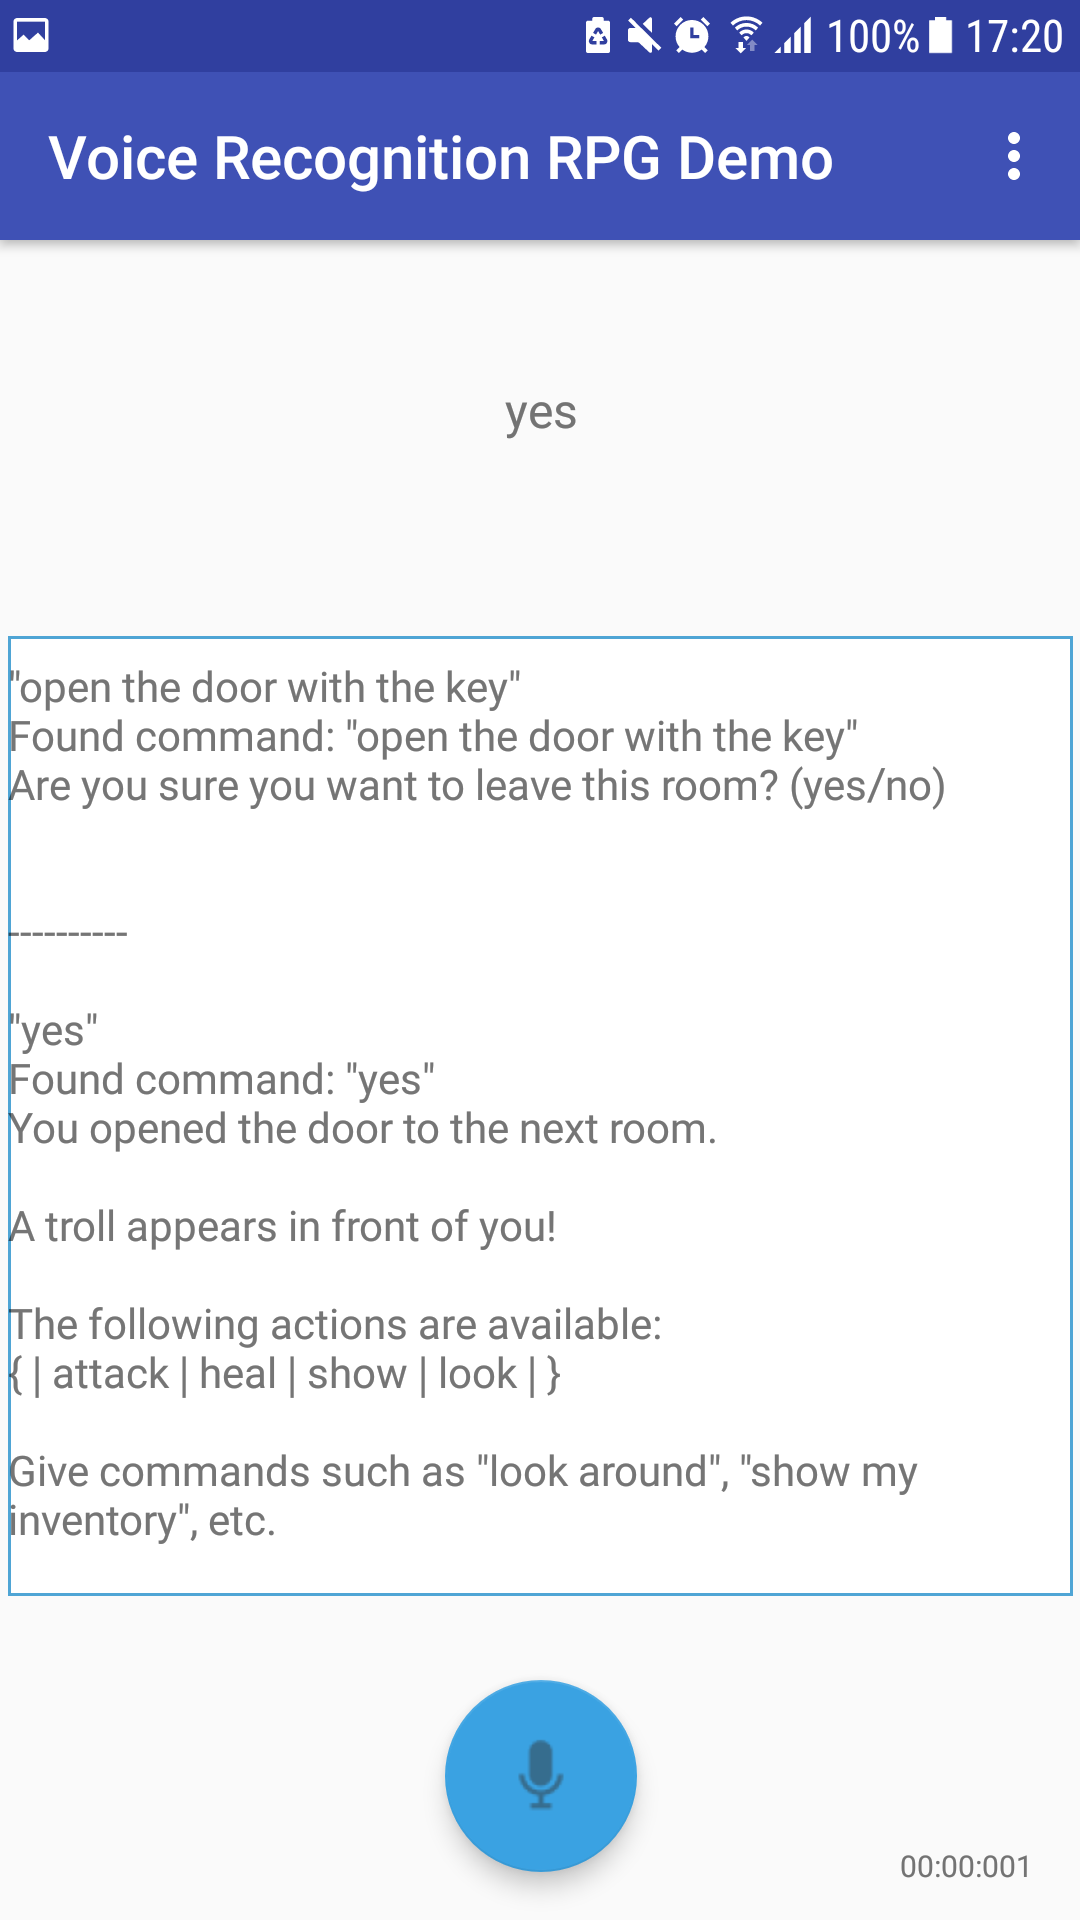
\includegraphics[scale=0.18]{overworld-4.png}
\end{center}

\newpage
\subsection{Multiple Commands Example}
\label{appendix:multiple-commands-ex}
The following is an example of a multiple-command intent being interrupted and then continued. In the first snapshot, the the system asks the user to resolve the first intent (``obliterate the troll using the sword"):

\begin{center}
\begin{figure}[H]
\begin{center}
  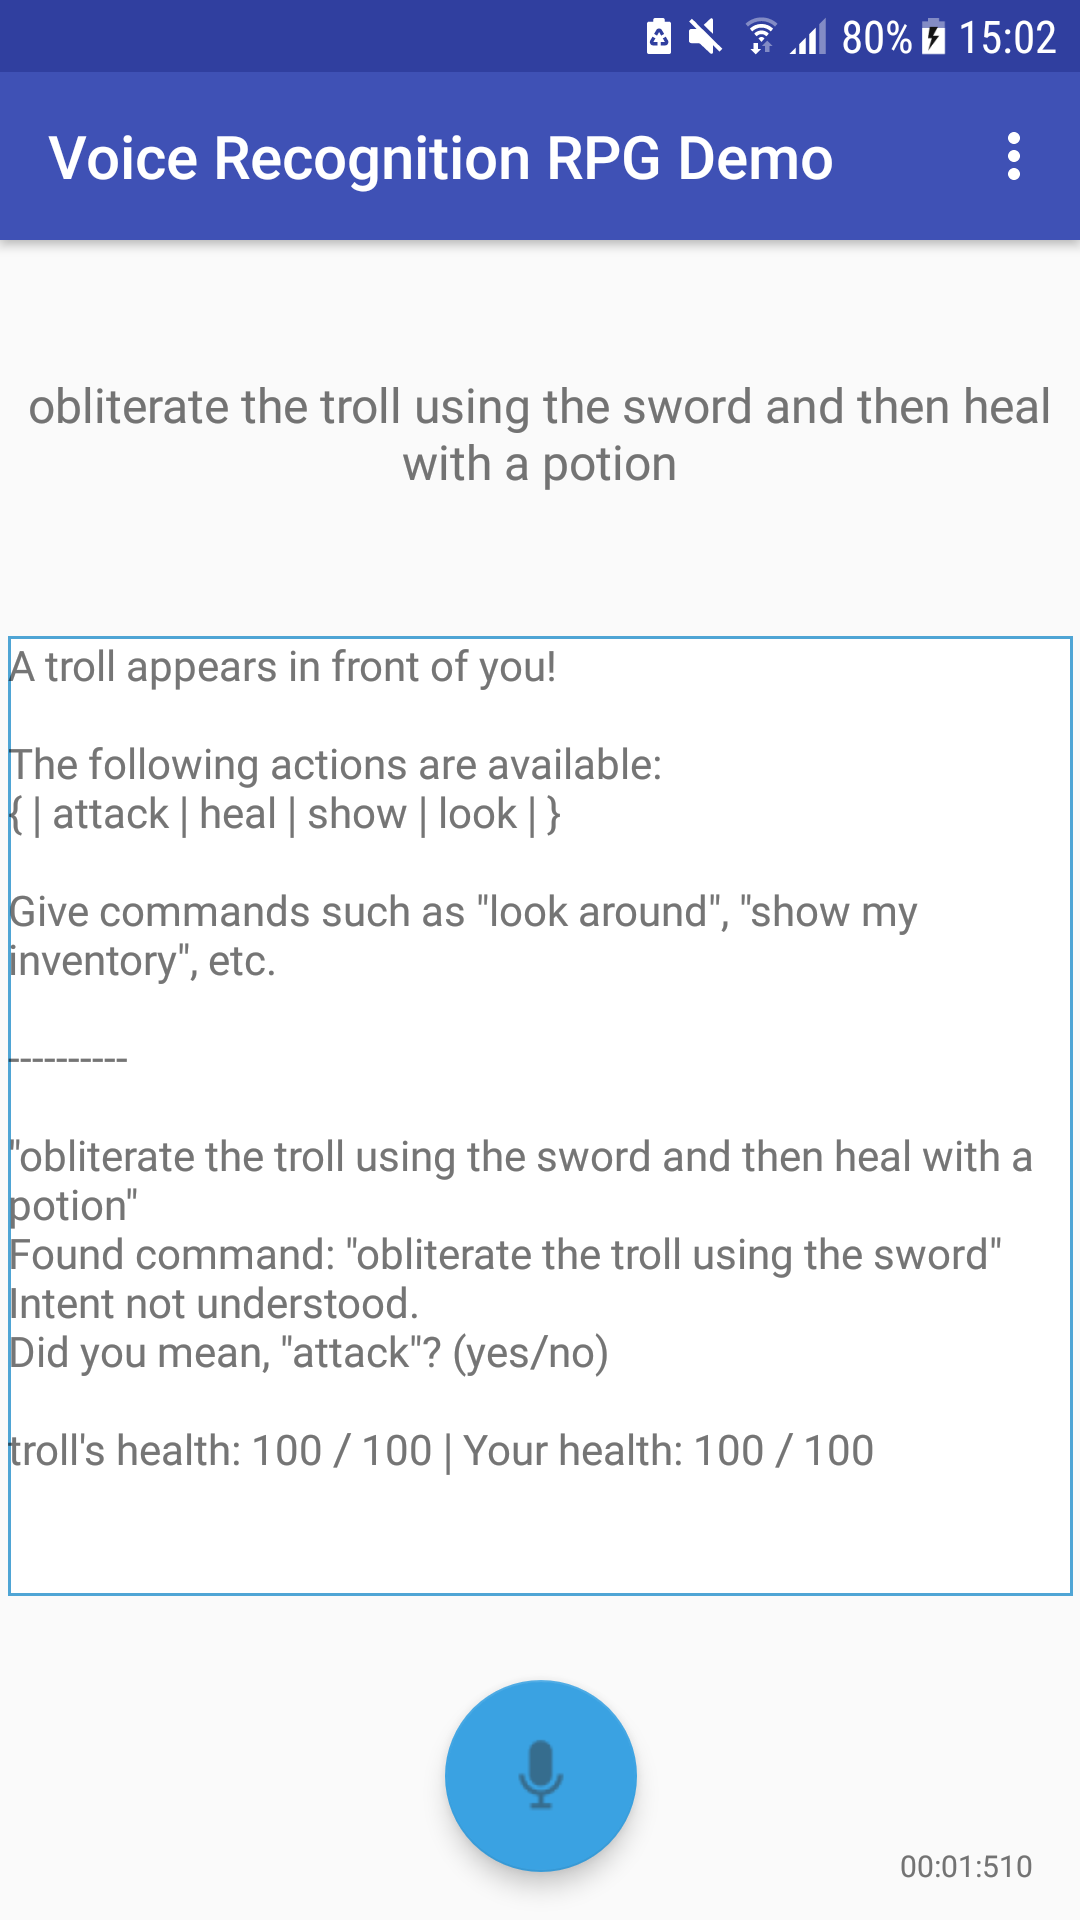
\includegraphics[scale=0.25]{Screenshot_20180527-150212.png}
  \label{fig:snapshot-multiple-command-1}
  \end{center}
\end{figure}
\end{center}

\newpage
Once the user resolves the first intent, it executes it followed by the second intent (``heal with a potion"):

\begin{center}
\begin{figure}[H]
\begin{center}
  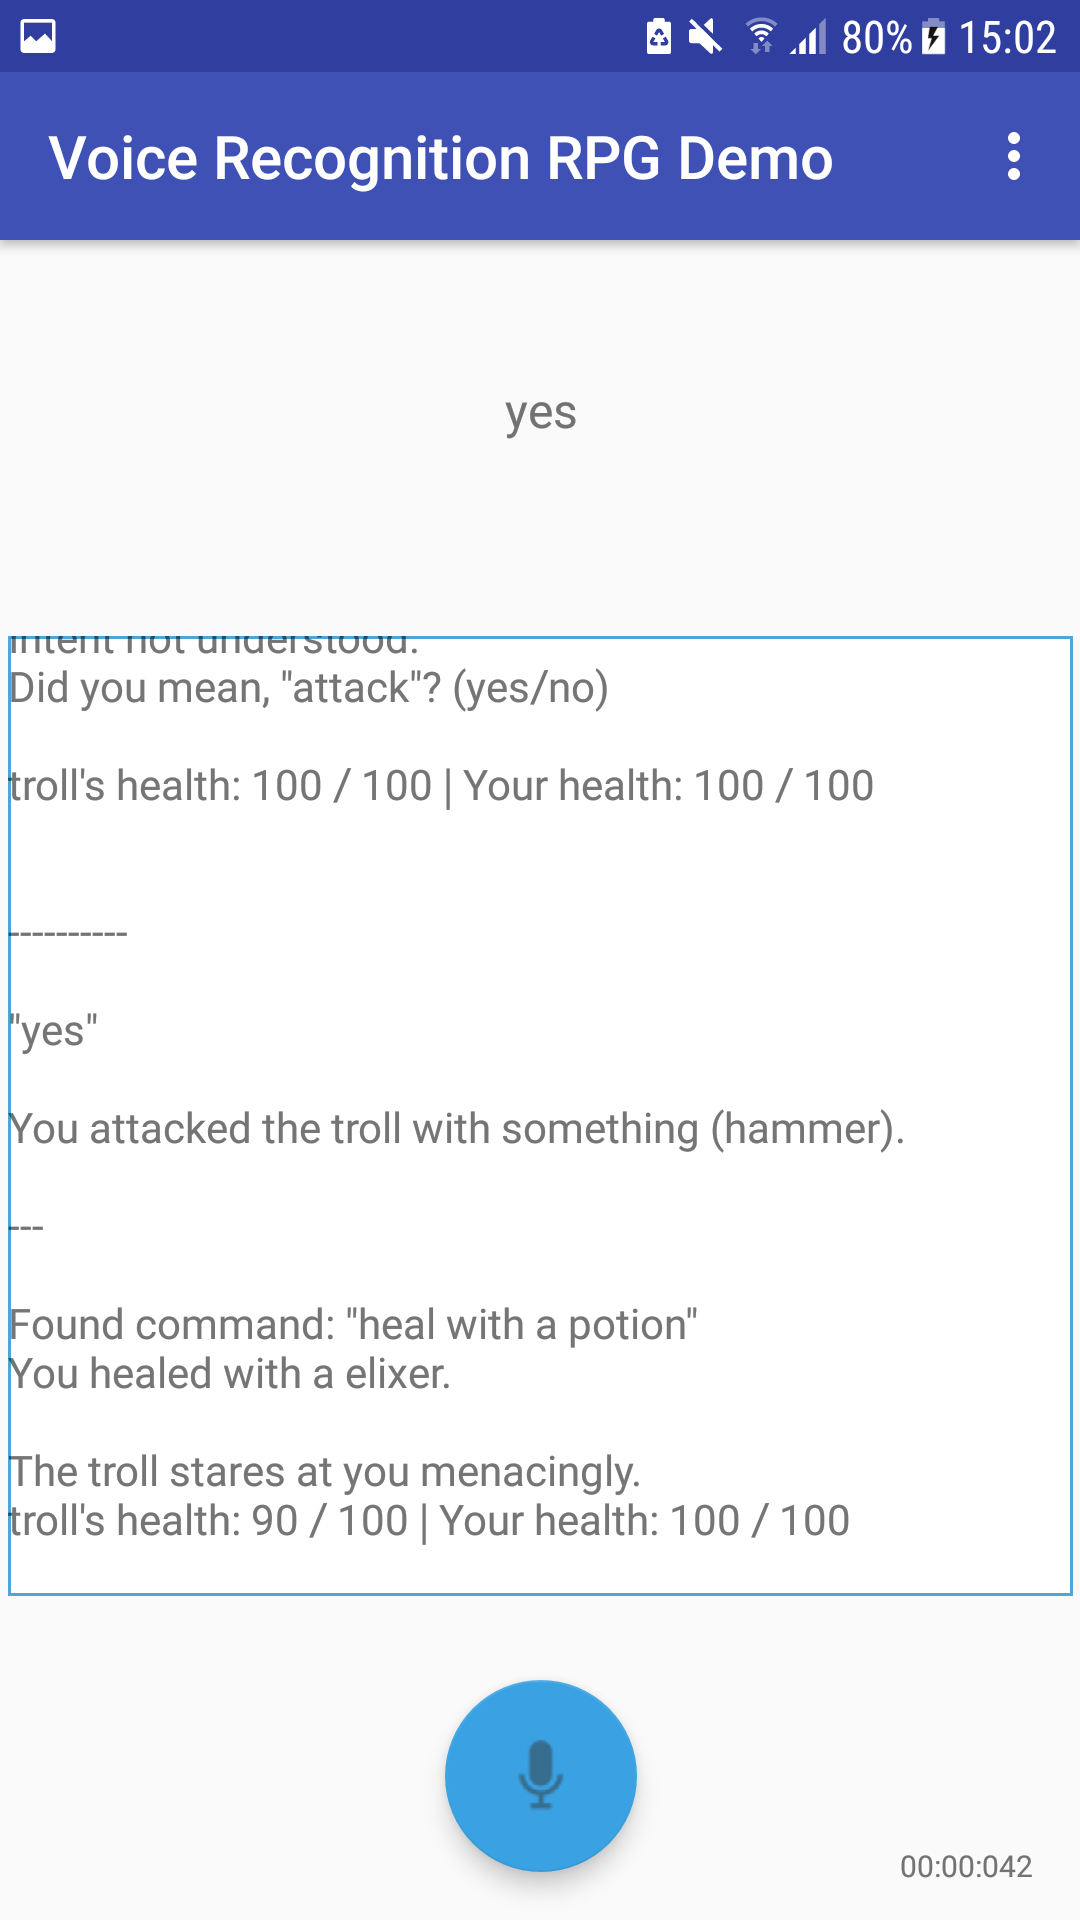
\includegraphics[scale=0.25]{Screenshot_20180527-150225.png}
  \label{fig:snapshot-multiple-command-2}
  \end{center}
\end{figure}
\end{center}

\newpage
\subsection{Ambiguous Utensil Example}
\label{appendix:utensil}
Below are screenshots of the room containing both a fork and a knife, with the synonym mapping of \texttt{utensil --> [fork, knife]} defined.

\begin{center}
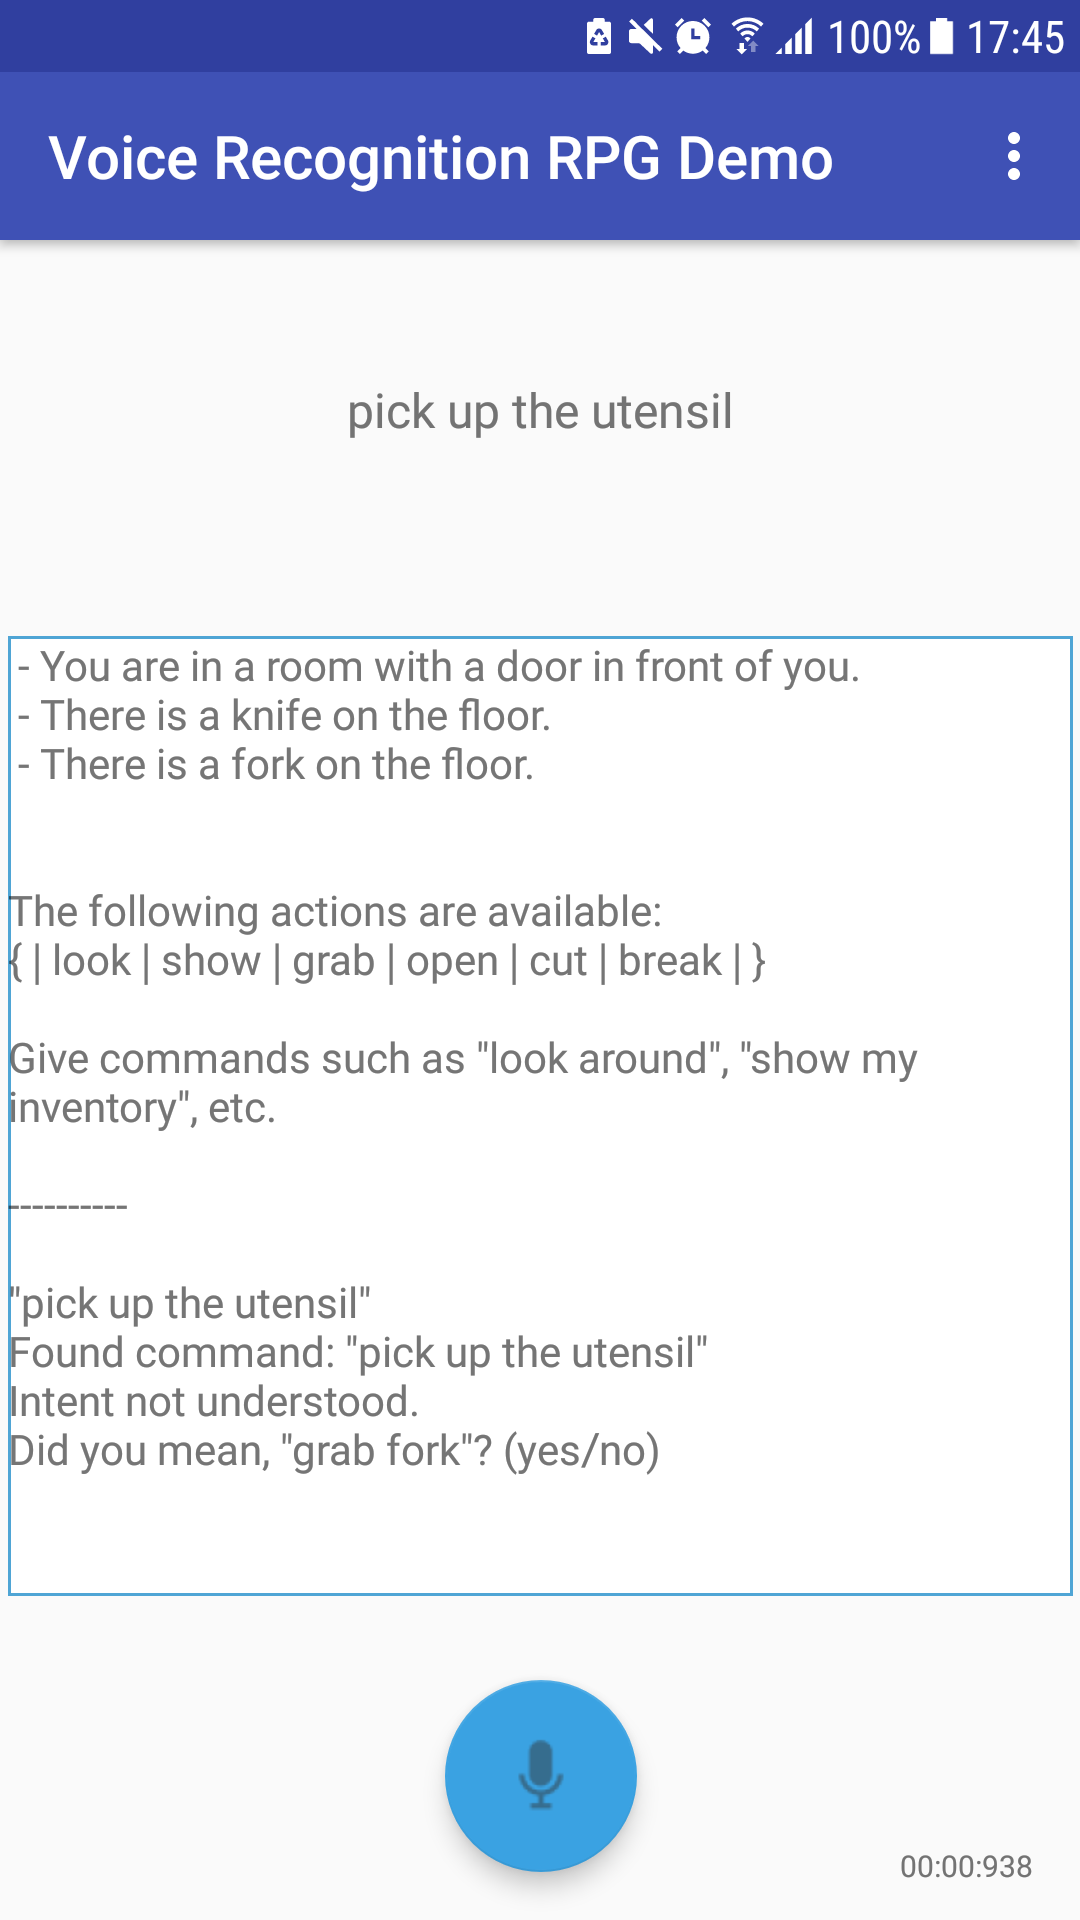
\includegraphics[scale=0.18]{utensil-1.png}
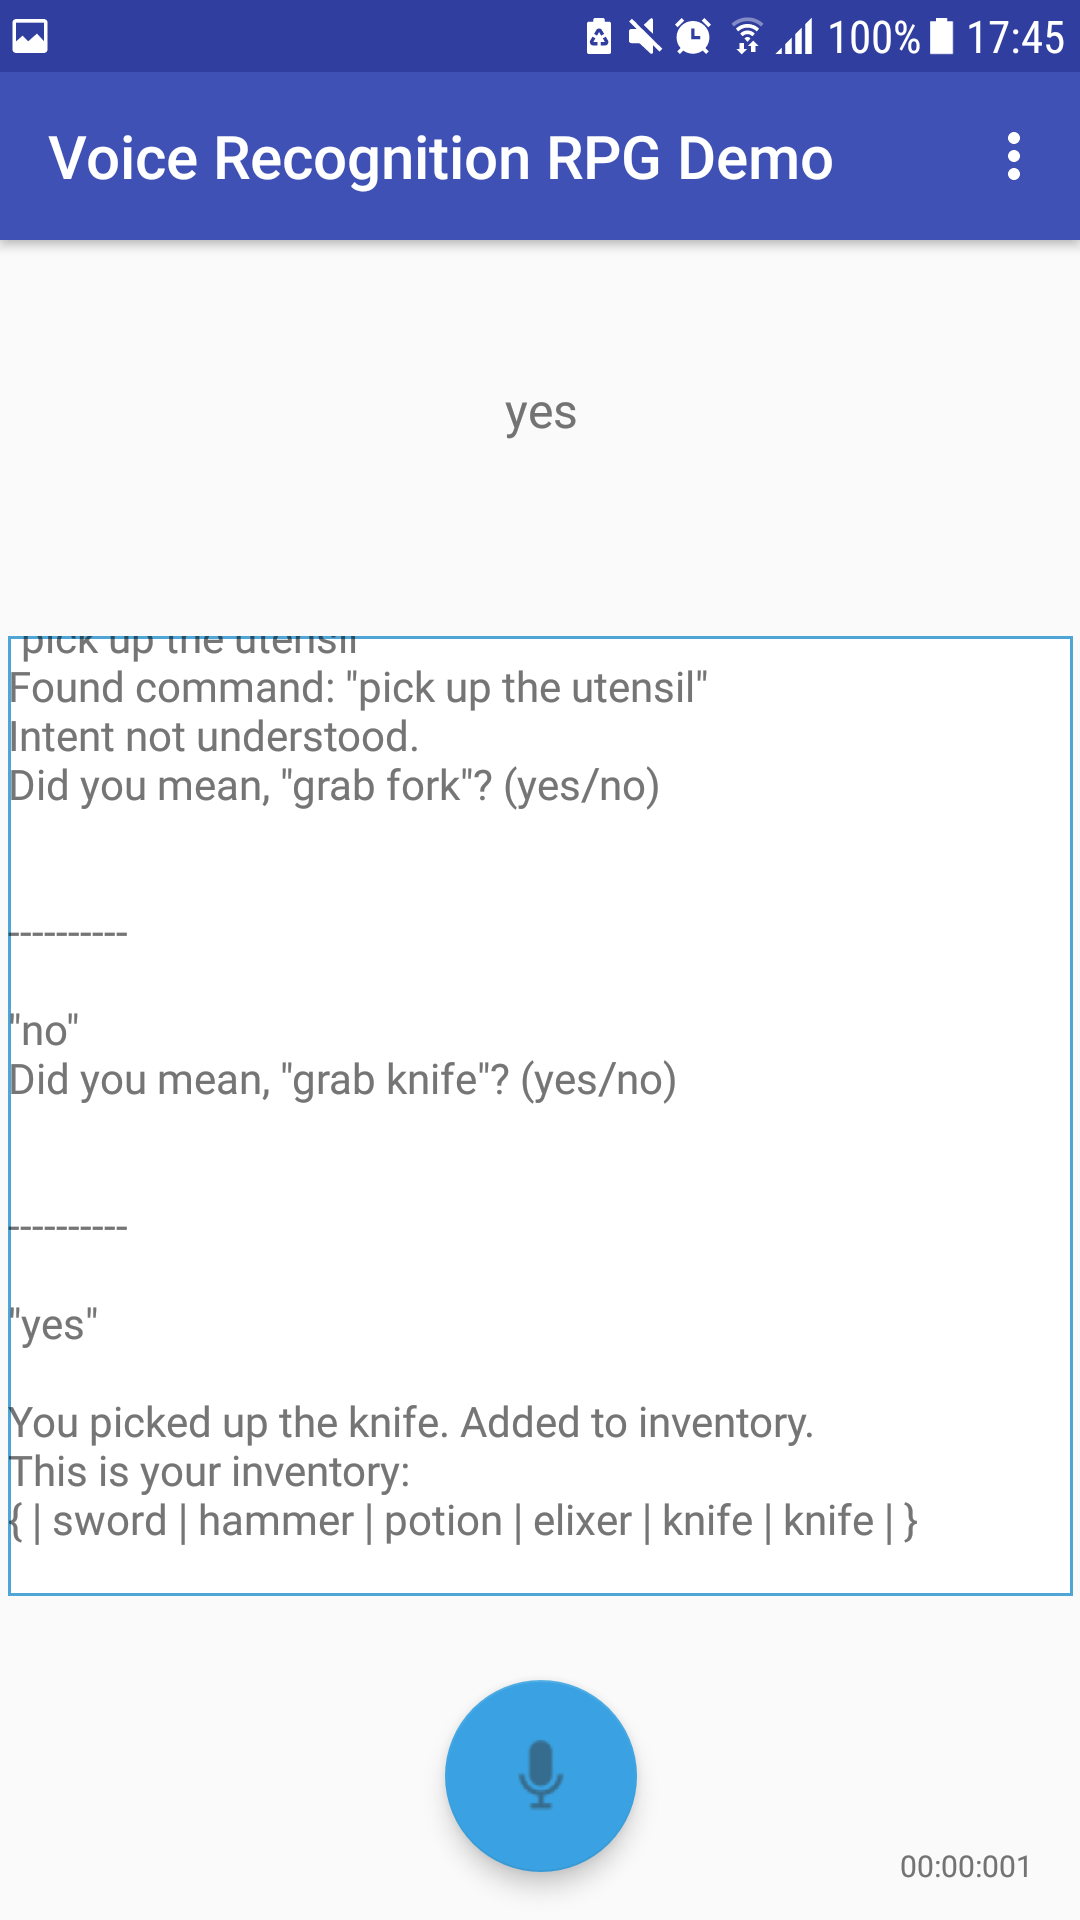
\includegraphics[scale=0.18]{utensil-2.png}
\end{center}

\newpage
If there are multiple mappings for utensil to various objects (e.g. \texttt{utensil --> [fork, knife, spoon, instrument]}), then all matches are dispalyed at the same time. Below is a screenshot of a room with these objects.

\begin{center}
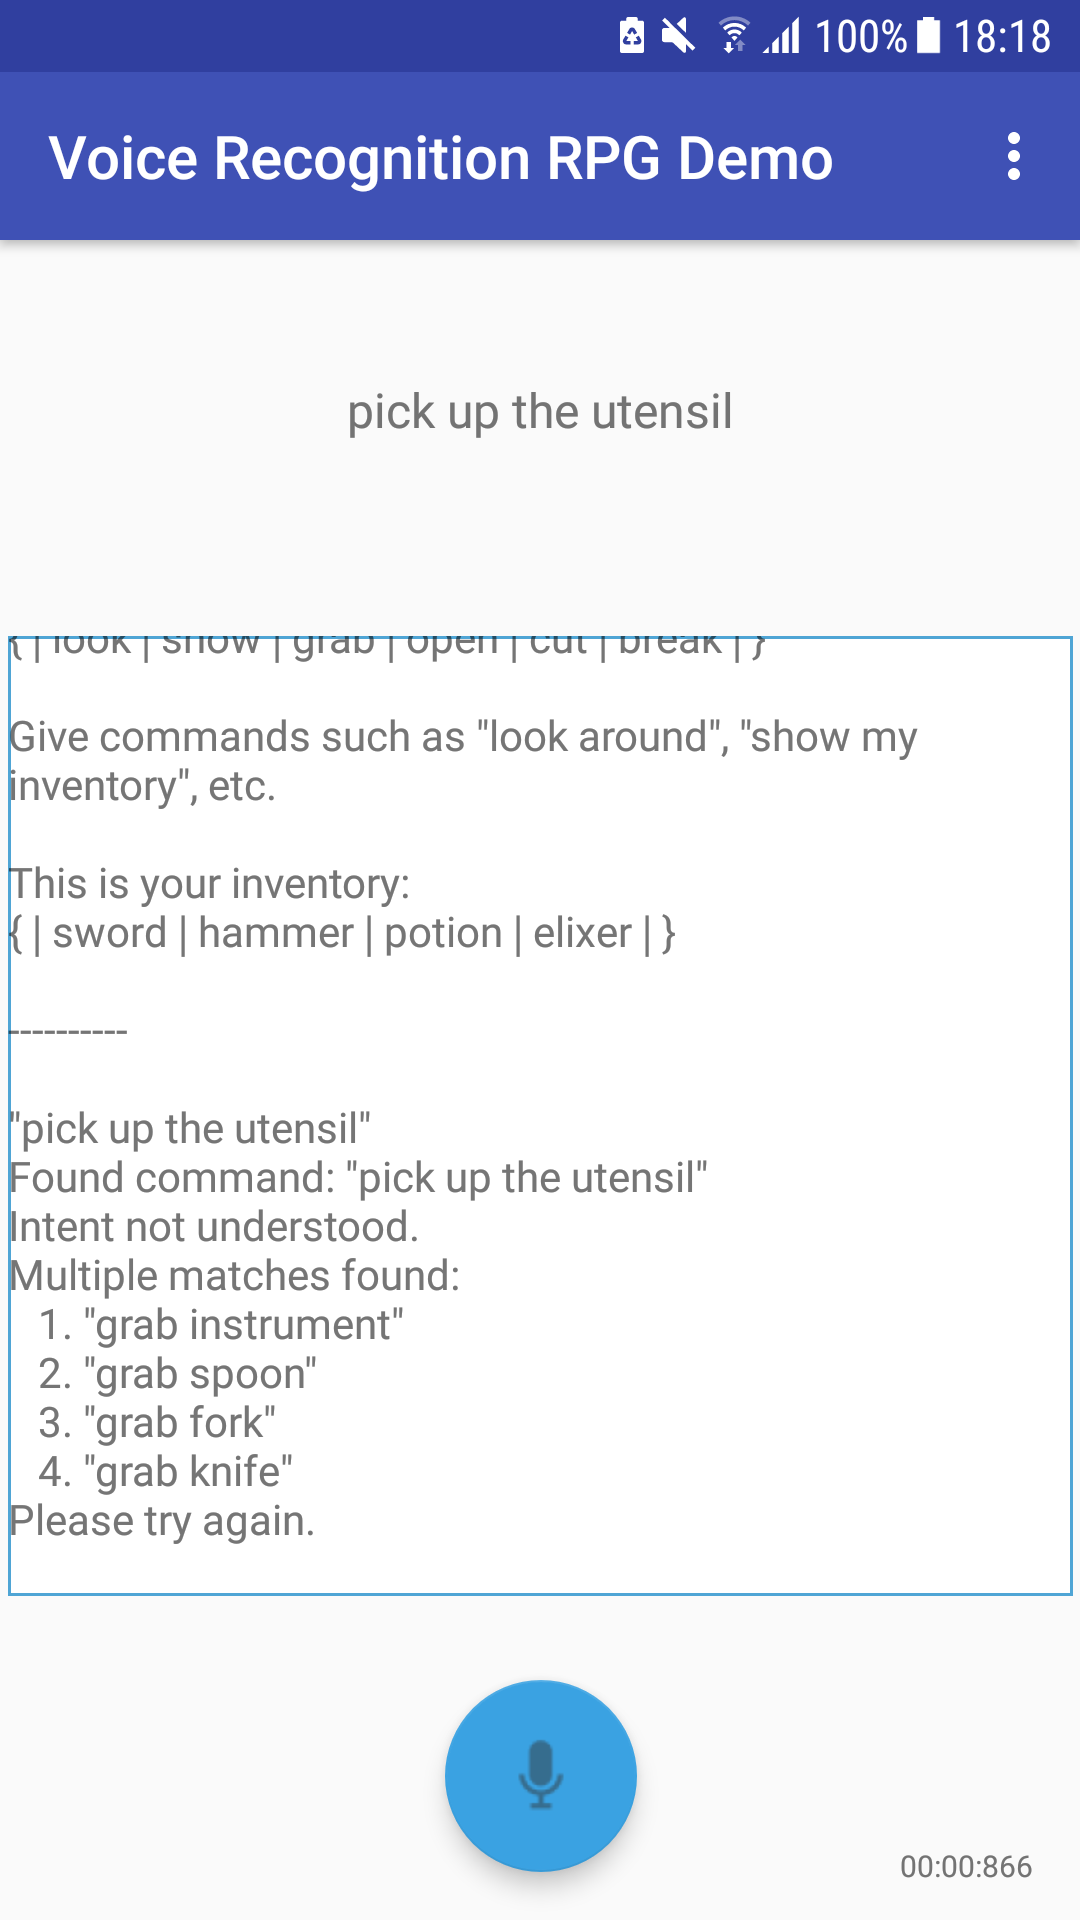
\includegraphics[scale=0.25]{utensil-3.png}
\end{center}

\newpage
\subsection{Settings User Interface}
\label{appendix:settings}
Below is a screenshot of the graphical user interface for the settings.

\begin{center}
\begin{figure}[H]
\begin{center}
  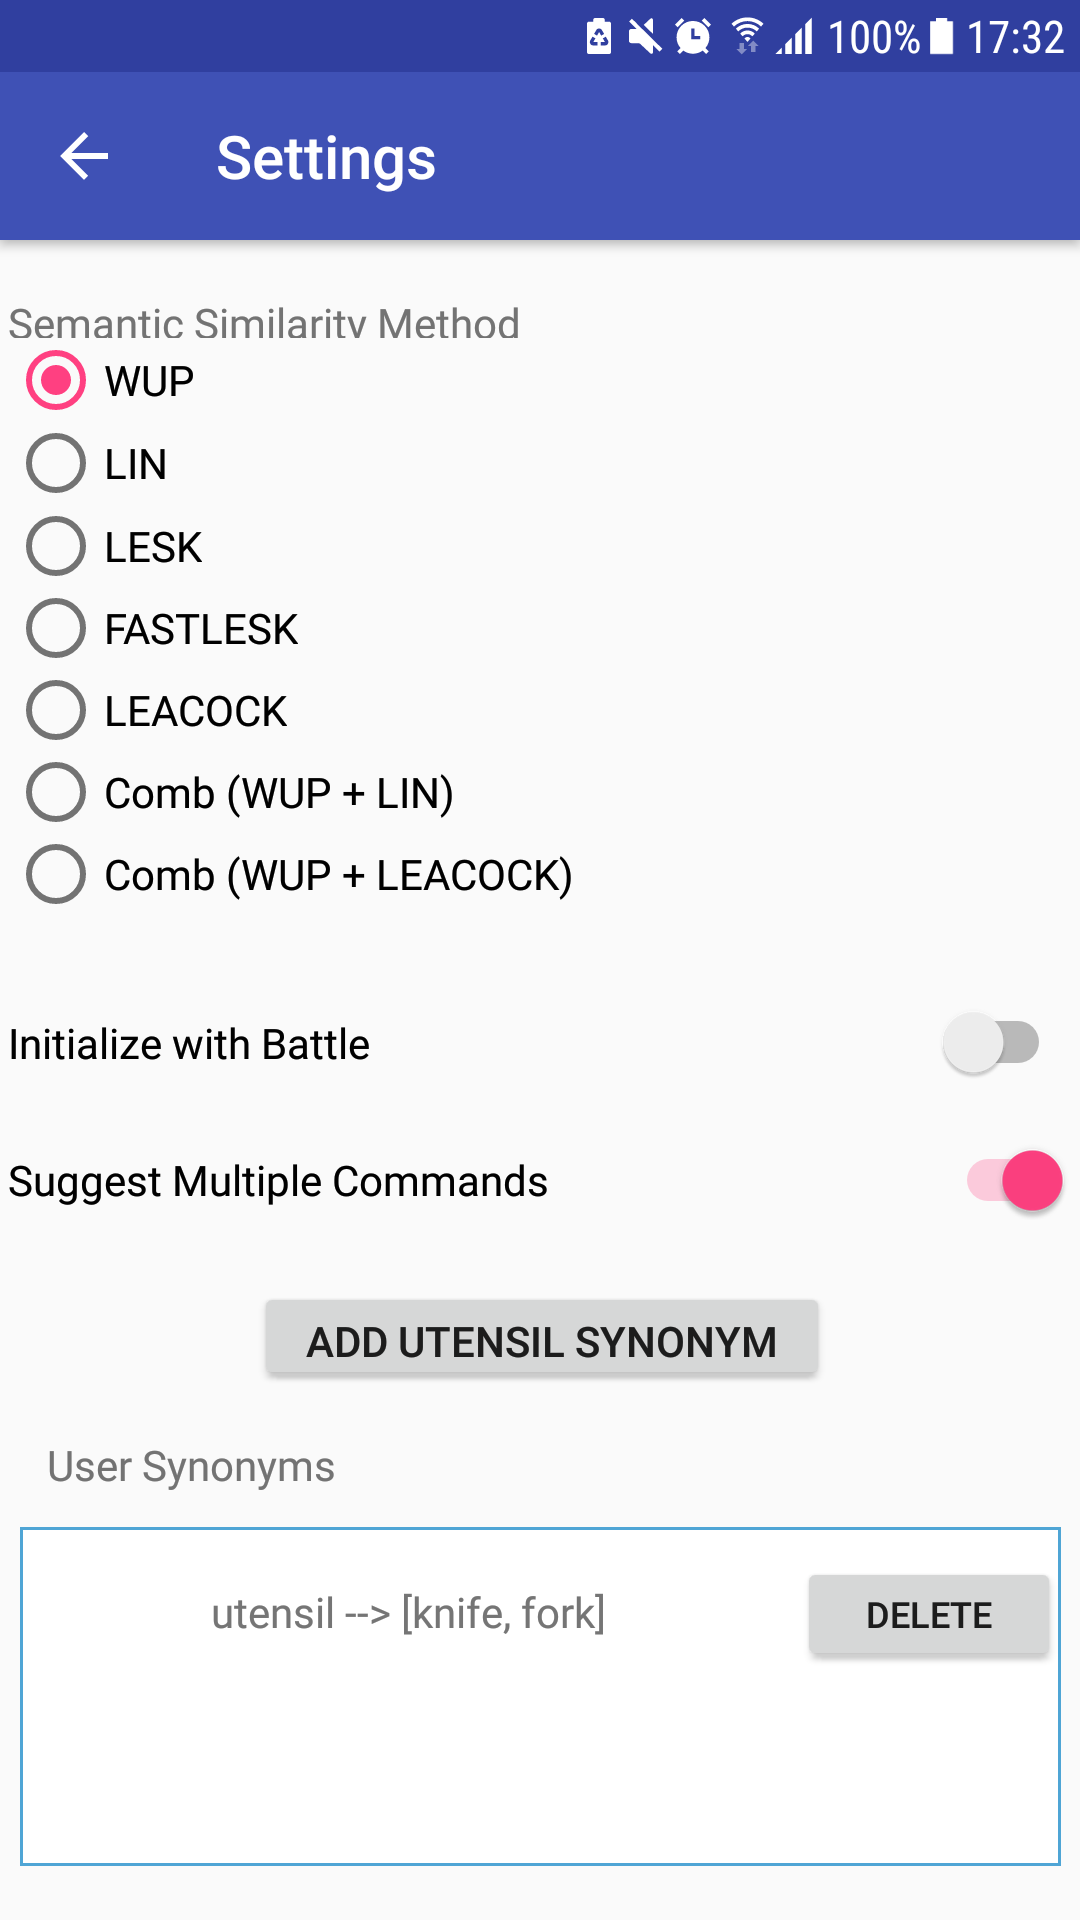
\includegraphics[scale=0.25]{settings.png}
  \caption{A snapshot of the settings activity.}
  \label{fig:snapshot-settings}
  \end{center}
\end{figure}
\end{center}

\newpage
\subsection{Duplicate Contacts}
\label{appendix:duplicate-contacts}
Below is a screenshot of the video conferencing demo when an ambiguous contact is called. The user would reply with the surname of the correct contact.

\begin{center}
\begin{figure}[H]
\begin{center}
  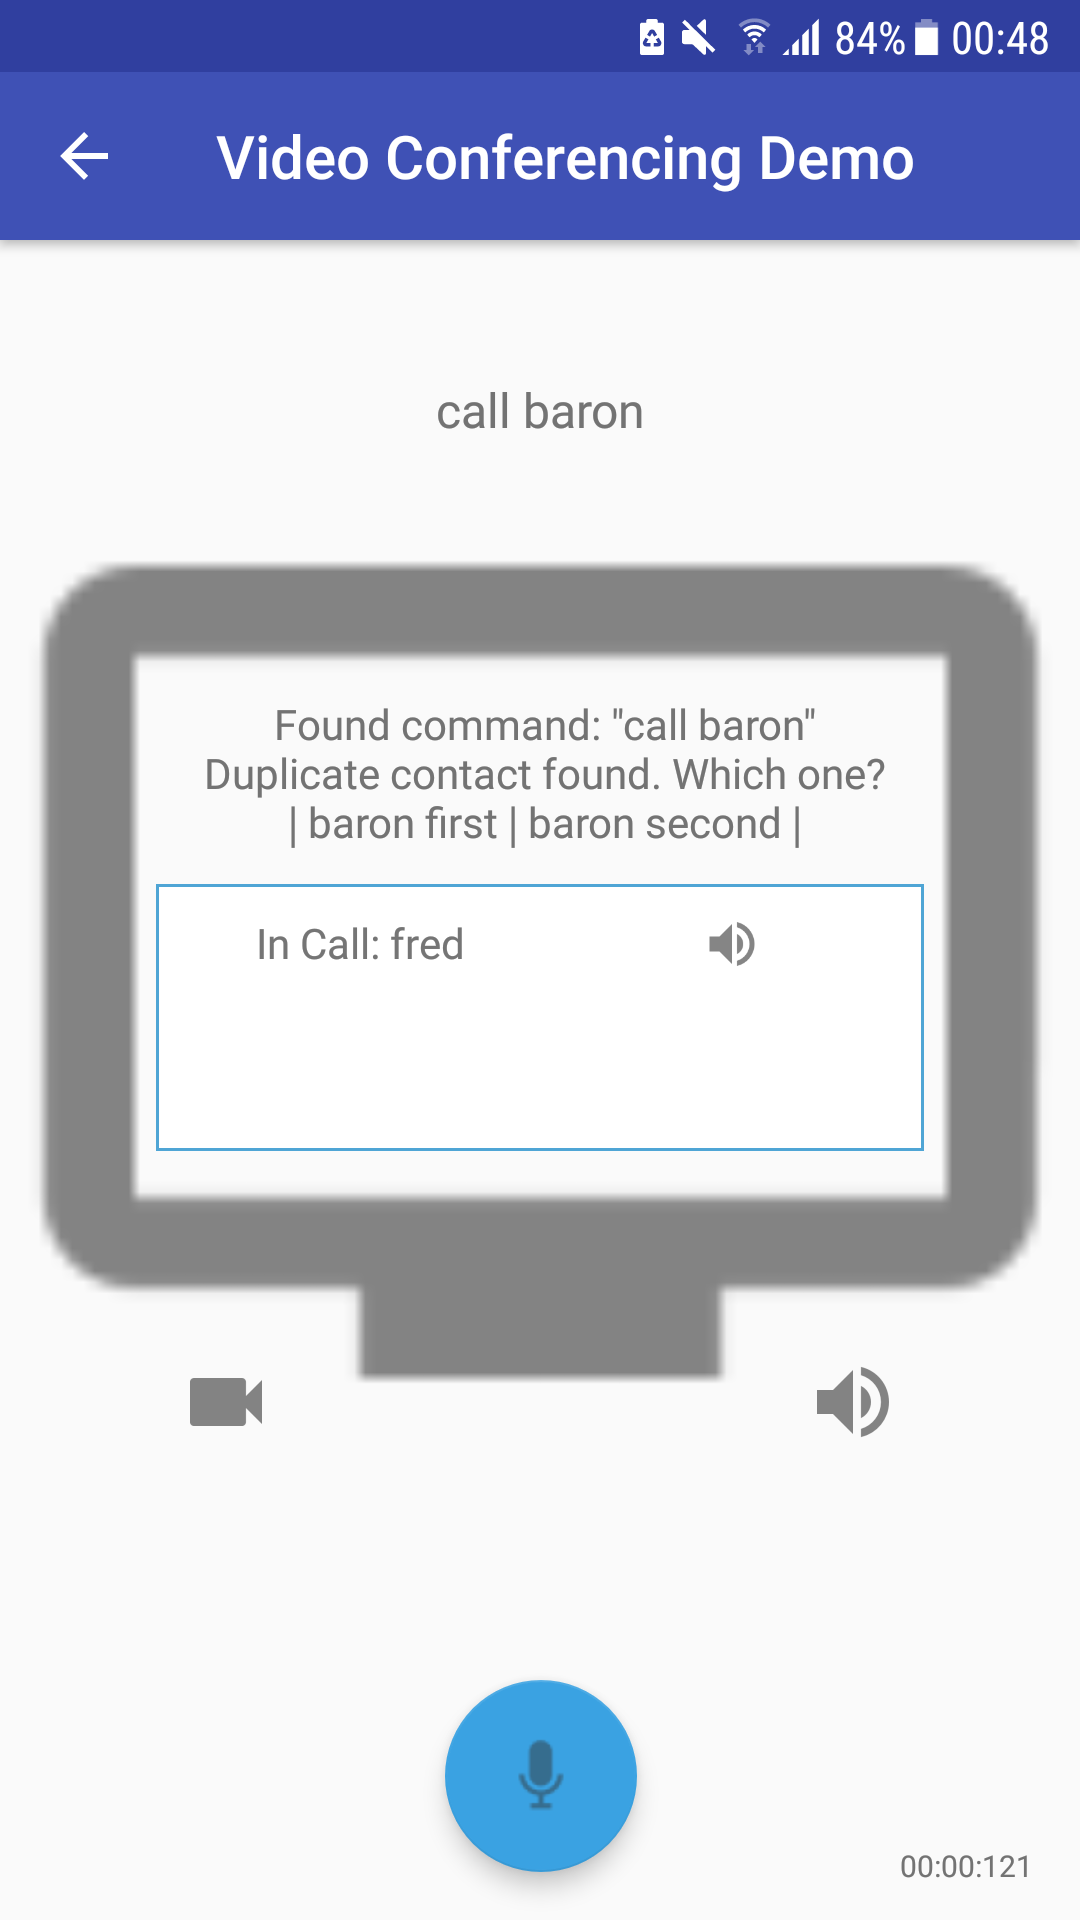
\includegraphics[scale=0.25]{duplicate-contacts.png}
  \caption{A snapshot of scenario involving duplicate contacts.}
  \label{fig:snapshot-duplicate-contacts}
  \end{center}
\end{figure}
\end{center}

\newpage
\section{Diagrams and Examples}
\subsection{System UML Class Diagram}
\label{appendix:system-uml}
Below is the UML class diagram for the voice recognition system used in the Android app. This was automatically generated using the third-party \textit{simpleUML} plugin for Android Studio \cite{RefWorks:108}.
\\
\\
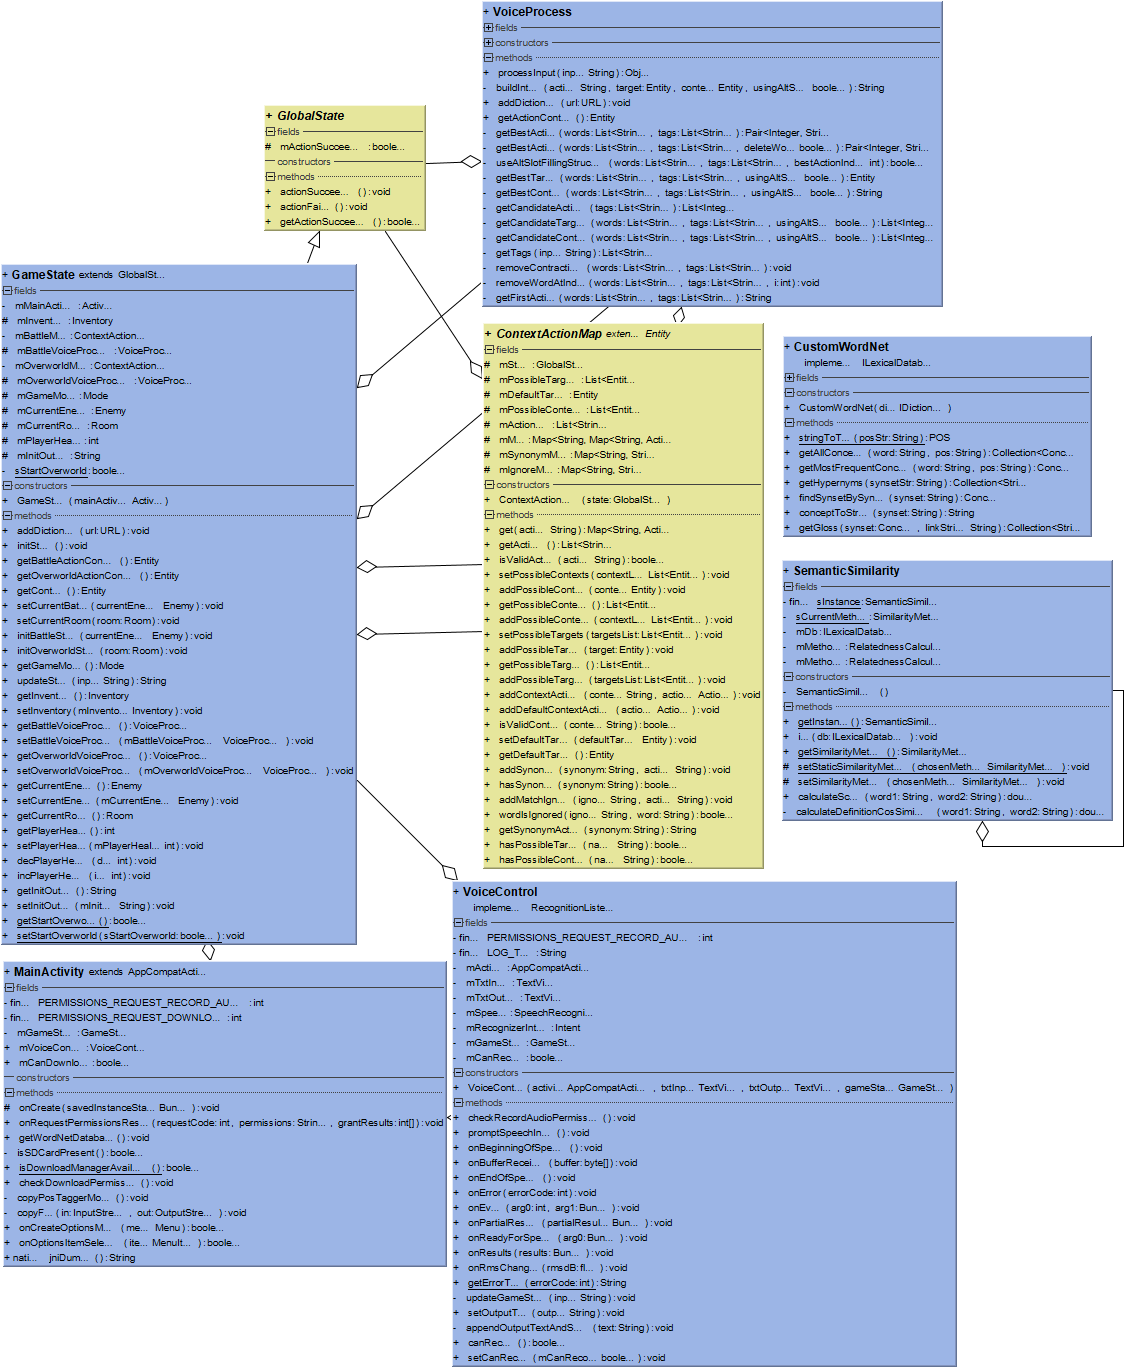
\includegraphics[scale=0.37]{system-uml.png}

\newpage
\subsection{Game Design UML Class Diagram}
\label{appendix:game-uml}
Below is the UML class diagram for the game mechanics - both the \textit{Overworld} and \textit{Battle} game modes. Generated using the third-party \textit{simpleUML} Android plugin.
\\
\\
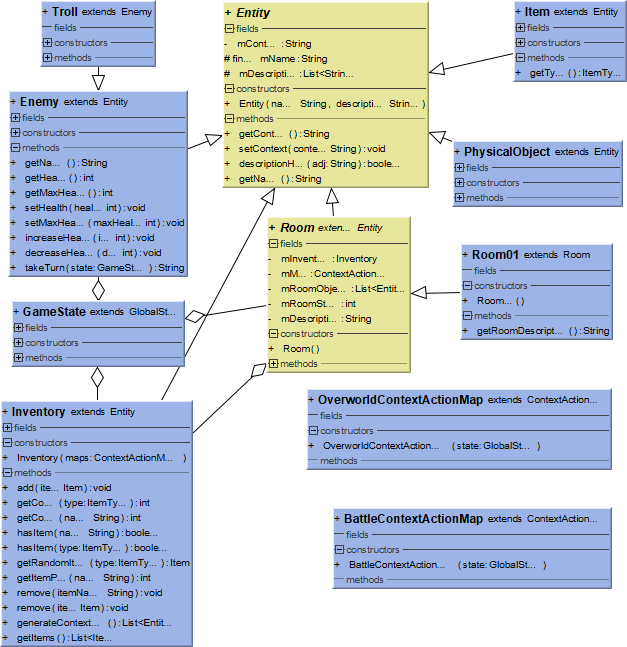
\includegraphics[width=\textwidth]{game-uml.png}

\newpage
\subsection{Battle Mode Example Commands}
\label{appendix:battle-examples}

Below is a table of some of the example commands that can be used in the \textit{Battle} mode of the role-playing game. Note that this is not an exhaustive list, and more commands are supported.

\begin{table}[H]
\centering
\begin{tabular}{|c|}
\hline
``attack with a hammer"                    \\ \hline
``punch the troll"   \\ \hline
``launch an assult"           \\ \hline
``heal with a potion"  \\ \hline
``show my inventory"      \\ \hline
``hit the troll with a bang"        \\ \hline
``obliterate the troll with a sword and then recover using a potion" \\ \hline
``fight with a sword and hammer"                      \\ \hline
``use the sword to attack"            \\ \hline
``what actions can i do"                \\ \hline
``what is in my bag"                    \\ \hline
``use a heavy attack"              \\ \hline
``launch an assault towards the troll using something sharp"             \\ \hline
\end{tabular}
\end{table}

\newpage
\subsection{Overworld Mode Example Commands}
\label{appendix:overworld-examples}

Below is a table of some of the example commands that can be used in the \textit{Overworld} mode of the role-playing game. Note that this is not an exhaustive list.

\begin{table}[H]
\centering
\begin{tabular}{|c|}
\hline
``look around the room"                    \\ \hline
``observe the surroundings"   \\ \hline
``slash the door using a knife"           \\ \hline
``break the table"  \\ \hline
``cut the painting"      \\ \hline
``pick up the potion"        \\ \hline
``grab the knife" \\ \hline
``scratch the door with the knife and then with the sword"                      \\ \hline
``use the knife to cut the table and the door"            \\ \hline
``use the key to open the door"                \\ \hline
``unlock the door"                    \\ \hline
``smash the table with the hammer"              \\ \hline
``look at the painting"             \\ \hline
\end{tabular}
\end{table}

\newpage
\subsection{Video Conferencing Example Commands}
\label{appendix:call-examples}

Below is a table of some of the example commands that can be used in the video conferencing demo within the application. As above, this is not an exhaustive list.

\begin{table}[H]
\centering
\begin{tabular}{|c|}
\hline
``call fred"                    \\ \hline
``phone jane with audio only"   \\ \hline
``call fred and jane"           \\ \hline
``use video only to call jane"  \\ \hline
``stop the call with fred"      \\ \hline
``stop all of the calls"        \\ \hline
``end all of the conversations" \\ \hline
``hang up"                      \\ \hline
``hang up with fred"            \\ \hline
``mute my video"                \\ \hline
``mute fred"                    \\ \hline
``unmute my audio"              \\ \hline
``silence my audio"             \\ \hline
\end{tabular}
\end{table}

Below is a table of all the available contacts in the demo:

\begin{table}[H]
\centering
\begin{tabular}{ll}
\textbf{First Name} & \textbf{Second Name} \\
Fred                & N/A                  \\
Jane                & N/A                  \\
Baron               & First                \\
Baron               & Second              
\end{tabular}
\end{table}

\newpage
\section{Testing and Evaluation}
\subsection{List of Android Mock Tests}
\label{appendix:mock-tests}

Below is a list of most of the test suites containing commands that are tested for correctness in the Android application. Note that commands that are tested for incorrectness, or any tests that are not testing commands, are not shown here. Also note that some test suites in \texttt{BattleTest} are repeated in \texttt{OverworldTest} (as they modes use different \texttt{ContextActionMap}s), so are not shown again, and any commands that are tested multiple times in the same test class are only shown once. Please see the project's repository for the full test framework.

\subsubsection{BattleTest}
\begin{scriptsize}
\begin{itemize}
\item testAttackInputSuite
	\begin{itemize}
	\item ``attack"
	\item ``attack with everything you have got"
	\item ``hit"
	\item ``hit the troll"
	\item ``punch the troll"
	\item ``launch an assault"
	\item ``charge at the troll"
	\item ``fight the troll"
	\item ``attack the troll"
	\item ``attack with the hammer"
	\item ``attack with the sledgehammer"
	\item ``attack the troll with the sledgehammer"
	\item ``use something to attack with"
	\item ``use a sword attack"
	\end{itemize}
\item testCorrectContexts
	\begin{itemize}
	\item ``attack the troll with a sword"
	\item ``attack the troll with a hammer"
	\end{itemize}
\item testHealInputSuite
	\begin{itemize}
	\item ``heal"
	\item ``use a potion to heal"
	\item ``heal with elixer"
	\item ``use an elixer right now before it is too late to heal"
	\item ``recover with an elixer"
	\item ``use something to heal with"
	\item ``heal myself with a potion"
	\end{itemize}
\item testDescriptions
	\begin{itemize}
	\item ``attack with something blunt"
	\item ``hit the troll with something pointy please"
	\item ``launch an assault towards the troll using something sharp"
	\item ``use a heavy attack"
	\end{itemize}
\item testInventorySuite
	\begin{itemize}
	\item ``show my inventory"
	\item ``show my bag"
	\item ``please show the contents of my possessions that I have"
	\item ``look at my inventory"
	\end{itemize}
\item testUseSuite
	\begin{itemize}
	\item ``use the sword to attack"
	\item ``use something to attack with"
	\item ``use a potion"
	\item ``use something sharp"
	\end{itemize}
\item testLookAroundSuite
	\begin{itemize}
	\item ``look around"
	\item ``look at the troll"
	\end{itemize}
\item testShowActionsSuite
	\begin{itemize}
	\item ``show my commands"
	\item ``look at my actions"
	\end{itemize}
\item testLearningSuite
	\begin{itemize}
	\item ``strike means attack"
	\item ``strike the troll"
	\end{itemize}
\item testConfirmation
	\begin{itemize}
	\item ``obliterate the troll with the sword"
	\item ``kick the troll"
	\item ``regenerate using a potion"
	\item ``use something to regenerate with"
	\item ``attack with a bang"
	\end{itemize}
\item testMultipleCommandsSuite
	\begin{itemize}
	\item ``obliterate the troll with the sword and then regenerate using a potion"
	\item ``attack with a sword and hammer"
	\item ``attack with a hammer and with a sword"
	\end{itemize}
\item testSentenceMatching
	\begin{itemize}
	\item ``what are my actions"
	\item ``what actions can i do"
	\item ``what is in my bag"
	\end{itemize}
\end{itemize}
\end{scriptsize}

\subsubsection{OverworldTest}
\begin{scriptsize}
\begin{itemize}
\item testLookSuite
	\begin{itemize}
	\item ``look at my inventory"
	\item ``look inside the bag"
	\item ``look around"
	\item ``look at the surroundings"
	\item ``observe the room"
	\end{itemize}
\item testPickUpSuite
	\begin{itemize}
	\item ``pick up the knife"
	\item ``grab the potion"
	\end{itemize}
\item testRoom01CutSuite
	\begin{itemize}
	\item ``cut the painting"
	\item ``cut the table using the knife"
	\item ``slash the door using the knife"
	\end{itemize}
\item testBreakSuite
	\begin{itemize}
	\item ``break the table"
	\item ``break the door"
	\end{itemize}
\item testOpenSuite
	\begin{itemize}
	\item ``open the table"
	\item ``open the door"
	\end{itemize}
\item testUseSuite
	\begin{itemize}
	\item ``use your hand to pick up the knife"
	\item ``use the knife to slash the door"
	\item ``use the knife to cut the glass table"
	\item ``use the knife to cut the painting"
	\item ``use the key to open the door"
	\end{itemize}
\item testMultipleCommandsSuite
	\begin{itemize}
	\item ``grab the knife and cut the painting then unlock the door"
	\end{itemize}
\item testMultipleCommandsAndMultipleSuggestionsSuite
	\begin{itemize}
	\item ``grab the utensil and then cut the painting with the knife"
	\end{itemize}
\item testMultipleTargetsSuite
	\begin{itemize}
	\item ``pick up the knife and the potion"
	\item ``break the table and the door"
	\end{itemize}
\item testMultipleTargetsWithContextSuite
	\begin{itemize}
	\item ``use the knife to cut the table and the door"
	\item ``cut the table with the knife and the door with the sword"
	\item ``cut the door with the knife and then with the sword"
	\end{itemize}
\item testMultipleSynonymMapping
	\begin{itemize}
	\item ``grab the utensil"
	\item ``pick up the utensil"
	\end{itemize}
\end{itemize}
\end{scriptsize}

\subsubsection{CallTest}

\begin{scriptsize}
\begin{itemize}
\item testCallingSuite
	\begin{itemize}
	\item ``call fred"
	\item ``call jane"
	\item ``phone jane"
	\item ``contact fred"
	\item ``call fred with video"
	\item ``use audio to phone jane"
	\item ``call fred and jane"
	\end{itemize}
\item testStopCallsSuite
	\begin{itemize}
	\item ``stop all the calls"
	\item ``end all of the conversations"
	\item ``stop call with jane"
	\item ``finish call with jane"
	\item ``hang up"
	\item ``hang up with fred"
	\item ``stop calling fred"
	\end{itemize}
\item testMutedSuite
	\begin{itemize}
	\item ``mute my video"
	\item ``mute my audio"
	\item ``unmute my video"
	\item ``unmute my audio"
	\item ``silence my audio"
	\item ``increase my audio"
	\item ``mute fred"
	\item ``unmute fred"
	\end{itemize}	
\end{itemize}
\end{scriptsize}

Please see the project's repository for the full test framework.

\newpage
\subsection{Actions and Contexts used in Evaluation}
\label{appendix:evaluation-context-action-maps}

Below are the \texttt{ContextActionMap} `tables' used in the evaluation Java project for the three domains. See the project's repository for the full classes.

\begin{table}[H]
\centering
\caption{GameContextActionMap}
\label{evaluation-game-table}
\begin{tabular}{l|l|l|l|l}
                 & \textbf{attack} & \textbf{heal} & \textbf{move} & \textbf{defend} \\ \hline
\textbf{default} & Attack          & Heal          & Move          & Defend          \\ \hline
\textbf{weapon}  & AtkWeapon       &               &               &                 \\ \hline
\textbf{potion}  &                 & HealPotion    &               &                 \\
\end{tabular}
\end{table}

\begin{table}[H]
\centering
\caption{CallContextActionMap}
\label{evaluation-call-table}
\begin{tabular}{l|l|l|l}
                 & \textbf{phone}    & \textbf{stop}   & \textbf{mute} \\ \hline
\textbf{default} & PhoneContact      & StopCall        & Mute          \\ \hline
\textbf{video}   & PhoneContactVideo &                 &               \\ \hline
\textbf{audio}   & PhoneContactAudio &                 &               \\ \hline
\textbf{contact} &                   & StopCallContact &               \\ 
\end{tabular}
\end{table}

\begin{table}[H]
\centering
\caption{CookingContextActionMap}
\label{evaluation-cooking-table}
\begin{tabular}{l|l|l|l|l|l}
                 & \textbf{make} & \textbf{stir} & \textbf{boil} & \textbf{pour} & \textbf{serve} \\ \hline
\textbf{default} & Make          & Stir          & Boil          & Pour          & Serve          \\ \hline
\textbf{spoon}   & Make          & StirSpoon     &               &               &                \\ \hline
\textbf{cooker}  & Make          &               & BoilCooker    &               &                \\ \hline
\textbf{food}    & MakeFood      &               &               &               &                \\
\end{tabular}
\end{table}

\newpage
\subsection{Comparison of Usability}
\label{appendix:comparison}

This section outlines a comparison between the usability of the voice recognition system implemented in this project, and other na\"ive/traditional systems. The example below is the same one used in the \texttt{README} file of the library's repository\footnote{https://github.com/BaronKhan/voice-commands-with-wordnet/blob/master/README.md}
\\
\\
If the user wished to map the following commands to an intent which attacked with a sword:

\begin{itemize}
\item ``attack with a sword"
\item ``hit with something sharp"
\item ``use a blade to fight"
\item ``launch an assault using the sword"
\item ``obliterate the enemy with a pointy weapon"
\end{itemize}

Or commands which mapped to healing with a potion:

\begin{itemize}
\item ``heal"
\item ``recover"
\item ``rest"
\item ``heal with a potion"
\item ``regenerate using a healing drink"
\end{itemize}

A na\"ive approach would be to use a switch statement\footnote{Strings can be evaluated with a \texttt{switch} statement since Java 7.} and add every possible variation of the command.

\begin{lstlisting}[language=Java]
switch(input) {
  case "attack with a sword":
  case "hit with something sharp":
  //...
  case "obliterate the enemy with a pointy weapon":
     attackWithWeapon();
     break;
  case "heal":
  case "recover":
  //...
  case "rest":
     heal();
     break;
  case "heal with a potion":
  case "recover with a potion":
  //...
  case "regenerate using an elixer":
     healWithPotion();
     break;
  //...
}
\end{lstlisting}

However, this misses out on other variations of the commands that would be acceptable (e.g. ``fight using a sword").
\\
\\
Another method is to create a regex-like expression to describe the structure of acceptable inputs:

\begin{lstlisting}
("attack" | "hit") . "with" . ["a"] . ("sword" | "blade")
\end{lstlisting}

However, this can also become quite complex, and still doesn't cover a wide variety of commands.

\begin{lstlisting}
("attack" | "hit" | "obliterate" | ("launch" . "an" . "assault")) . ("with" | "using") . ["a"] . ("sword" | "blade" | ("something" . ("pointy" | "sharp")))
\end{lstlisting}

With the system proposed in this project, the developer only has to create the following table of mappings in order to map all of the above commands and much more.

\begin{table}[H]
\centering
\label{comparison-table}
\begin{tabular}{l|l|l|l}
                 & \textbf{attack} & \textbf{heal} & \textbf{move} \\ \hline
\textbf{default} & Attack          & Heal          & Move          \\ \hline
\textbf{weapon}  & AtkWeapon       &               &                 \\ \hline
\textbf{potion}  &                 & HealPotion    & \\
\end{tabular}
\end{table}

Therefore, the number of lines needed to add the above voice commands and can be considered reduced using this method compared to the other two methods.

\newpage
\subsection{Other Survey Results}
\label{appendix:survey-results}

This section presents the other results from the anonymous survey given to developers. It should be noted that the same size for the survey is only eight participants, and the survey is intended to be supplementary information.

\begin{center}
\begin{figure}[H]
\begin{center}
  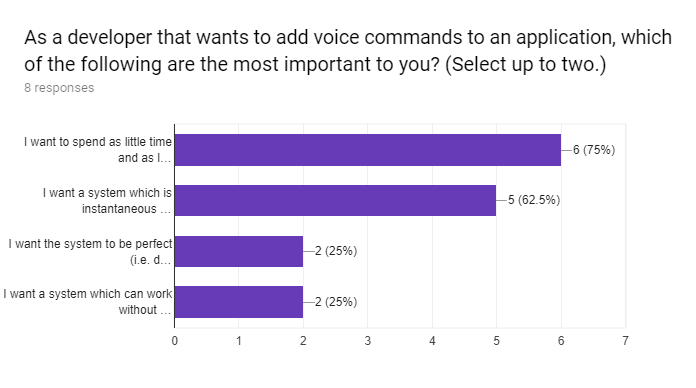
\includegraphics[width=\linewidth]{survey-important}
  \caption{A bar chart showing the responses when asking developers what are the most important aspects of a system for adding voice commands to an application.}
  \label{fig:survey-important}
  \end{center}
\end{figure}
\end{center}

\begin{center}
\begin{figure}[H]
\begin{center}
  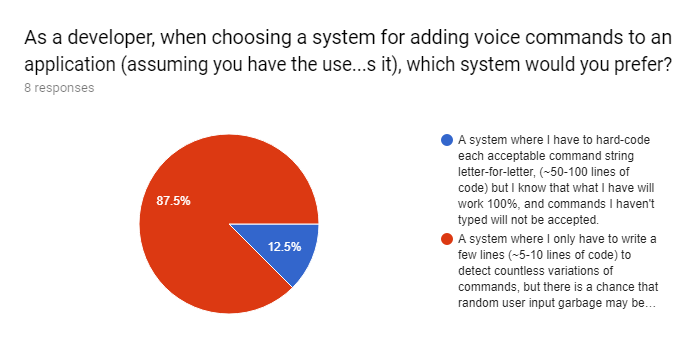
\includegraphics[width=\linewidth]{survey-tradeoff}
  \caption{A pie chart showing the responses to a question asking a developer about which type of voice recognition system they would prefer.}
  \label{fig:survey-tradeoff}
  \end{center}
\end{figure}
\end{center}

\begin{center}
\begin{figure}[H]
\begin{center}
  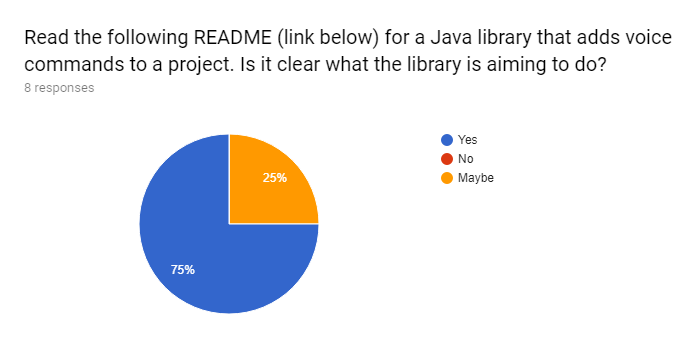
\includegraphics[width=\linewidth]{survey-readme}
  \caption{A pie chart showing the responses to a question asking a developer if they understood the purpose of the voice recognition system in making it easier to add voice commands.}
  \label{fig:survey-readme}
  \end{center}
\end{figure}
\end{center}

\newpage
\subsection{Room Generation Evaluation Results}
\label{appendix:room-generation-results}

The following is a text file for a room description (with each sentence contain an object relation), followed by the methods in the constructor from the output of the program:
\\
\\
``There is a *table in the room. A *knife is on the table. There is a *spoon on top of the table. A *fork lays on the table. There is a *chair under the table. A *letter sits upon the table. A *key is placed above the letter. A *sword is next to the table. A *hammer is with the sword. There is a *potion is underneath the table. An *elixer is beside the potion."

\begin{lstlisting}[language=Java]
addDescriptionWithObject(
    "There is a table in the room.",
    new GlassTable());
addDescriptionWithObjectCond(
    "A knife is on the table.",
    "A knife is now on the floor.",
    new Weapon("knife"),
    () -> getRoomObjectCount("table") > 0);
addDescriptionWithObject(
    "There is a spoon on top of the table.",
    new Weapon("spoon"));
addDescriptionWithObject(
    "A fork lays on the table.",
    new Weapon("fork"));
addDescriptionWithObject(
    "There is a chair under the table.",
    new Chair());
addDescriptionWithObjectCond(
    "A letter sits upon the table.",
    "A letter is now on the floor.",
    new Item("letter", Item.ItemType.ITEM_KEY, "document"),
    () -> getRoomObjectCount("table") > 0);
addDescriptionWithObjectCond(
    "A key is placed above the letter.",
    "A key is in the room.",
    new Item("key", Item.ItemType.ITEM_KEY, "access"),
    () -> getRoomObjectCount("letter") > 0);
addDescriptionWithObjectCond(
    "A sword is next to the table.",
    "A sword is in the room.",
    new Weapon("sword"),
    () -> getRoomObjectCount("table") > 0);
addDescriptionWithObjectCond(
    "A hammer is with the sword.",
    "A hammer is in the room.",
    new Weapon("hammer"),
    () -> getRoomObjectCount("sword") > 0);
addDescriptionWithObjectCond(
    "There is a potion is underneath the table.",
    "A potion is in the room.",
    new Potion("potion"),
    () -> getRoomObjectCount("table") > 0);
addDescriptionWithObjectCond(
    "An elixer is beside the potion.",
    "An elixer is in the room.",
    new Potion("elixer"),
    () -> getRoomObjectCount("potion") > 0);
\end{lstlisting}

Out of the 10 relations in the description, 7 of them are extracted by the program.

\newpage
\section{Supplementary Materials}
\subsection{Skyrim Kinect Command List}
\label{appendix:skyrim}
Below is a list of all 200 commands that can be used in the video game, The Elder Scrolls V: Skyrim, when a Microsoft Kinect peripheral is connected \cite{RefWorks:24}.

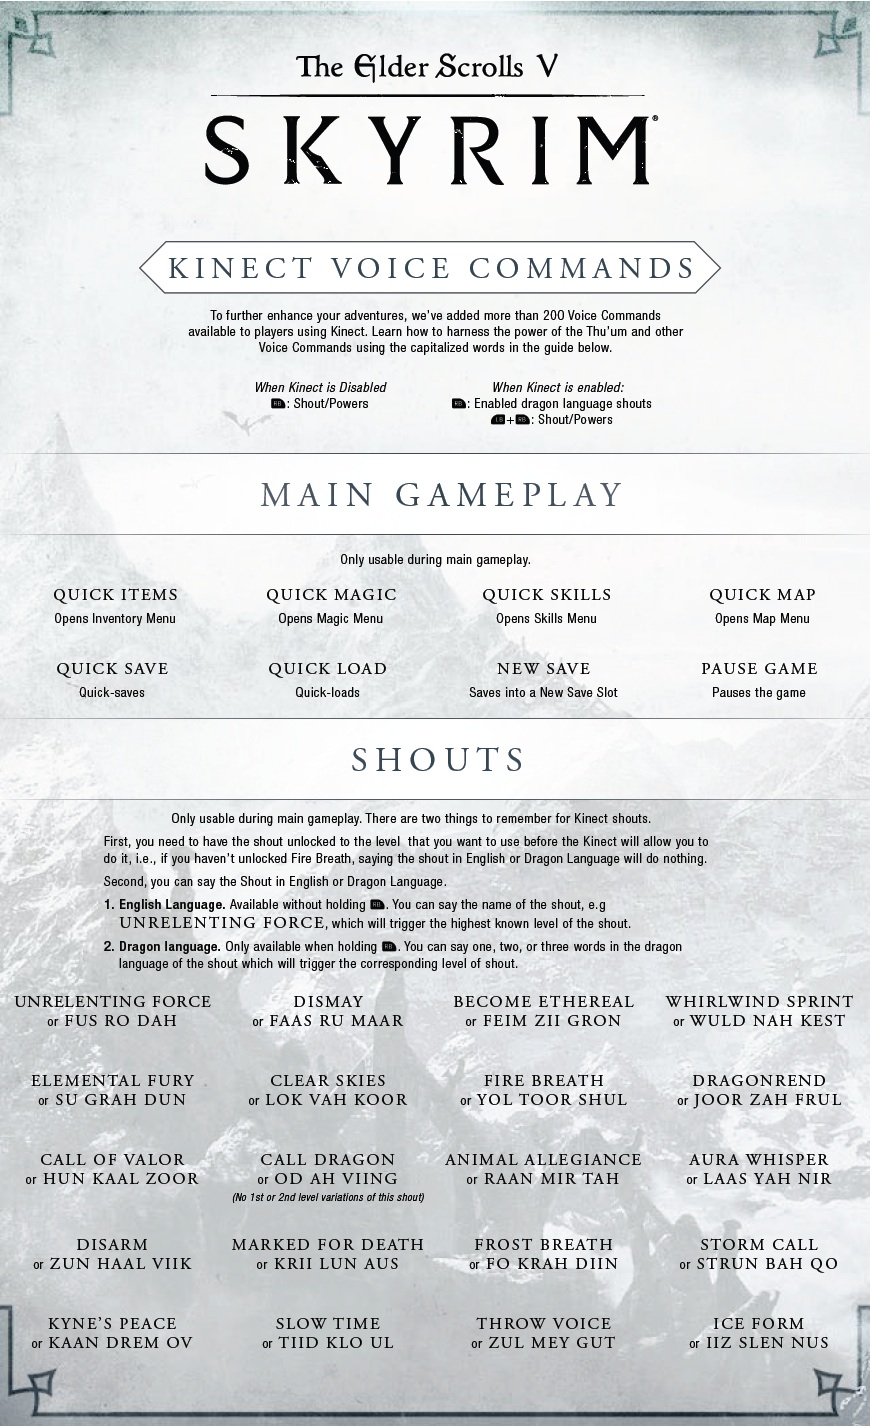
\includegraphics[scale=0.235]{skyrim-1.jpg}
\includegraphics[scale=0.235]{skyrim-2.jpg}
\newpage
\includegraphics[scale=0.237]{skyrim-3.jpg}
\includegraphics[scale=0.237]{skyrim-4.jpg}
\newpage
\subsection{Penn Treebank Tagset}
\label{appendix:penn}

Below is a table of the 32 tags from the Penn Treebank tagset, used for POS tagging. The 12 remaining tags for punctuation and other symbols have been left out \cite{RefWorks:42}.

$$
\begin{tabular}{ |p{3.25cm}|p{3.25cm}|p{3.25cm}|p{3.25cm}| }
\hline
	CC & Coordinating\ conjunction & TO & to \\ \hline
	CD & Cardinal\ number & UH & Interjection \\ \hline
	DT & Determiner & VB & Verb, base\ form \\ \hline
	EX & Existential\ there & VBD & Verb, past\ tense \\ \hline
	FW & Foreign\ word & VBG & Verb, gerund\ or\ present\ participle \\ \hline
	IN & Preposition\ or\ subordinating conjunction & VBN & Verb, past\ participle \\ \hline
	PRP\$ & Possessive\ pronoun & NNS & Noun,\ plural \\ \hline
	RB & Adverb & NNP & Proper\ noun,\ singular \\ \hline
	RBR & Adverb,\ comparative & NNPS & Proper\ noun, plural \\ \hline
	RBS & Adverb,\ superlative & PDT & Predeterminer \\ \hline
	RP & Particle & POS & Possessive\ ending \\ \hline
	SYM & Symbol & PRP & Personal\ pronoun \\ \hline
	JJ & Adjective & VBP & Verb, non-3rd\ person\ singular\ present \\ \hline
	JJR & Adjective, comparative & VBZ & Verb, 3rd\ person\ singular\ present \\ \hline
	JJS & Adjective,\ superlative & WDT & Wh-determiner \\ \hline
	LS & List\ item\ marker & WP & Wh-pronoun \\ \hline
	MD & Modal & WP\$ & Possessive\ wh-pronoun \\ \hline
	NN & Noun,\ singular\ or\ mass & WRB & Wh-adverb \\ \hline
\end{tabular}
$$

\newpage

\end{appendices}
\newpage
\addcontentsline{toc}{section}{References}
\bibliography{references}
\end{document}
